% This file was converted to LaTeX by Writer2LaTeX ver. 1.6.1
% see http://writer2latex.sourceforge.net for more info
\documentclass[11pt]{article}
\usepackage{amsmath,amssymb,amsfonts}

%\usepackage[a4paper, total={17cm, 26cm}]{geometry}
\usepackage[a4paper,margin=1.5cm]{geometry}
\usepackage{color}
\usepackage{hyperref} % Pour liens internets cliquables
\hypersetup{
    colorlinks=true,
    linkcolor=blue,
    filecolor=magenta,      
    urlcolor=blue, %cyan
    pdftitle={Cours de physique - DLPP - 2022},
    %pdfpagemode=FullScreen,
    }

\usepackage{hyperref}
\usepackage[
    type={CC},
    modifier={by-nc-sa},
    version={3.0},
]{doclicense}

\usepackage{multicol}
\setlength{\columnsep}{0.5cm}
\def\columnseprulecolor{\color{black}}

% pour les pieds de page et entêtes
\usepackage{fancyhdr}

\pagestyle{fancy}
\fancyhf{}
\lhead{Cours de physique}
\rhead{Oscillateur harmonique}
\lfoot{En cours de rédaction et correction - ne pas distribuer - \ccbyncsa}
\rfoot{Page \thepage}

\usepackage{pgfplots}
\pgfplotsset{compat=1.15}
\usepackage{mathrsfs}
\usetikzlibrary{arrows}

\usepackage{fontspec}
\usepackage{xunicode}
\usepackage{xltxtra}
\usepackage{array}
\usepackage{hhline}
\usepackage{graphicx}
\usepackage{polyglossia}
\usepackage{longtable}

\setdefaultlanguage{french}

\providecommand{\tightlist}{%
  \setlength{\itemsep}{0pt}\setlength{\parskip}{0pt}}
  
\newcounter{Text}
\renewcommand\theText{\arabic{Text}}
\title{Cours de physique de $6^e$ secondaire - 2021-2022 \\
En cours de rédaction et correction - ne pas distribuer \\
tout commentaire bienvenu par email à \\
 manueldephysique@educode.be}
\author{Alexandra David - Corinne Leyssen - Nicolas Pettiaux - Matteo Poncé}

\includeonly{
COURS_01-Energie-travail-puissance-rendement.tex,
%COURS_02-Energie-OHEXERCRESOL.tex,
%COURS_02-Energie_OH.tex
%COURS_03-Longueur_d_onde_et_ondes_progressives.tex,
%COURS_04_-Intensité_sonore.tex,
%COURS_05_-Réflex-Réfract+exerc_résolus.tex
%COURS_06-Diffraction_+_exercices(résolus).tex
%COURS_07-Interférences+exerc(résolus).tex
%COURS_08-Effet_Doppler.tex
%COURS_09-Expérience_de_Young.tex
%COURS_10-Diffraction_lumière_par_réseau.tex
%COURS_11-Réfraction_de_la_lumière.tex
%COURS_12-Indice_de_réfraction_lumière.tex
%COURS_13_-Ondes_électromagnétiques.tex
%COURS_14_-Effet_photoélectrique_et_lumière.tex
%COURS_15_-Energie_nucléaire.tex
%COURS_16__-thermodynamique.tex
%COURS__-Diffraction_de_la_lumière_par_un_réseau+_exerc_résolus.tex
}


\begin{document}
\maketitle
\doclicenseThis

\setcounter{tocdepth}{10}
\renewcommand\contentsname{Table des matières}
\tableofcontents

\hrulefill




\section{Énergie, travail, puissance et rendement}

\begin{multicols}{2}

\subsection{Travail d'une force}

Lorsqu'une force $\vec{F}$ déplace un corps sur une
distance $\vec{d}$, on dit que cette force effectue un
travail $W$.

Le travail de la force $\vec{F}$ sur la
distance $\vec{d}$ est définie par~: $W = \vec{F} \cdot \vec{d} = Fd\cos(\theta)$

L'unité du travail est celle de l'énergie : le joule $J$.
1 J = 1 N.m  Il s'agit donc d'une unité définie dans le 
\href{https://fr.wikipedia.org/wiki/Système_international d unités}{Système international d'unités, le SI}.

\begin{figure}
\centering
\definecolor{qqwuqq}{rgb}{0,0.39215686274509803,0}
\begin{tikzpicture}[line cap=round,line join=round,>=triangle 45,x=1cm,y=1cm]
\clip(-3.1072727272727243,-8.697272727272729) rectangle (19.001818181818166,6.593636363636364);
\draw [shift={(0,0)},line width=2pt,color=qqwuqq,fill=qqwuqq,fill opacity=0.10000000149011612] (0,0) -- (0:0.5454545454545451) arc (0:38.659808254090095:0.5454545454545451) -- cycle;
\draw [->,line width=2pt] (0,0) -- (5,4);
\draw [->,line width=2pt] (0,0) -- (12,0);
\begin{scriptsize}
\draw[color=black] (2.3290909090909078,2.5118181818181817) node {$F$};
\draw[color=black] (7.5109090909090845,0.366363636363636) node {$d$};
\draw[color=qqwuqq] (1.5654545454545445,0.4936363636363633) node {$\alpha$};
\end{scriptsize}
\end{tikzpicture}
%\includegraphics[width=3cm]{dessins/produit-scalaire.png}
\caption{Produit scalaire de la force $\vec{F}$ et de la distance $\vec{d}$. }
\end{figure}

TODO insérer un schéma de produit scalaire

Quelques exemples découlent de ces définitions~:
\begin{itemize}
\item   Une force n'effectue de travail que lorsque son point d'application se
  déplace. Par exemple, la force
musculaire d'un haltérophile effectue un travail lorsqu'il soulève une
haltère mais n'en n'accomplit
plus pendant qu'il la maintient à bout de bras au-dessus de la tête.
\item   \textbf{Le travail d'une force est une grandeur scalaire} obtenue à
  partir de deux grandeurs vectorielles $\vec{F}$ et  $\vec{d}$.
\item   On parle de \textbf{travail moteur} lorsque $\alpha < 90°$ et donc
  $ \cos(\alpha) > 0$. Le travail d'une force motrice est donc 
  généralement positif.
\item   On parle de \textbf{travail résistant} lorsque $\alpha > 90°$ et
  donc $\cos(\alpha) < 0$. Le travail d'une force de frottement est 
  donc généralement négatif.
\item   \textbf{Une force perpendiculaire au déplacement} ($\alpha = 90°$)
  \textbf{n'effectue aucun travail}.
C'est le cas de la force centripète du mouvement circulaire. Par exemple la 
force gravité qui retient la Lune tournant autour de la Terre. C'est aussi le cas 
de la force de pesanteur lors d'un déplacement horizontal.
\item   Le travail fait sur un objet est l'aire sous la courbe de la force
  agissant sur l'objet en fonction de la position .

  TODO ajouter une graphe F(t) et $\int_a^b \vec{F} \cdots \vec{dx}$ et des explications 
  
\end{itemize}


\begin{figure}
\centering
\includegraphics[width=12.989cm,height=3.115cm]{Pictures/1000000100000709000001B0D92B14C6C126C9B7.png}
\caption{}
\end{figure}

\begin{figure}
\centering
\includegraphics[width=7.292cm,height=4.895cm]{Pictures/100000010000031F00000218321A1B2B64E50C1E.png}
\caption{}
\end{figure}

(Sur le schéma~: (x'-x) = d)

\section{Énergie}

\subsection{Définition}
On définit \textbf{ l'énergie est la capacité que
possède un corps à produire un travail. Son unité le Joule (J).}

La notion d'énergie est sans doute la plus importante de la physique. 
TODO à expliquer

\subsection{Différentes formes d'énergie~: }

\begin{itemize}
\item cinétique liée à la vitesse et à la masse d'un corps
\item potentielle liée à la masse d'un corps et à la hauteur à laquelle il
se trouve. (g est l'accélération de pesanteur).
\item mécanique égale la somme : Ecinétique + Epotentielle
\item thermique liée à la température d'un corps
\item électrique liée à l'électricité
\item chimique liée aux liaisons chimiques entre les atomes
\item rayonnante liée aux ondes électromagnétiques : la lumière,
l'infrarouge, l'ultraviolet etc.
\item nucléaire liée aux liaisons des protons et neutrons dans les noyaux
d'atomes
\item de masse liée à la masse selon la relation d'Einstein : $E = m c^2$, 
la formule sans doute la plus connue de tous, mais sans doute aussi mal 
comprise.
\end{itemize}



\section{Puissance }

En \href{https://fr.wikipedia.org/wiki/Physique}{physique},
la puissance reflète la vitesse à laquelle un
\href{https://fr.wikipedia.org/wiki/Travail_d\%27une_force}{\emph{\emph{travail}}}
est fourni.

\emph{Définition}~: C'est la quantité
d'\href{https://fr.wikipedia.org/wiki/\%C3\%89nergie_(physique)}{\emph{\emph{énergie}}}
fournie par unité de temps.

Son unité est le watt (w) (Remarque~: ne confondez pas le travail (W) et
le watt (w).

La puissance est une grandeur scalaire.

La puissance correspond donc à un débit d'énergie~: si deux systèmes de
puissances différentes fournissent \textbf{le même
}\href{https://fr.wikipedia.org/wiki/Travail_d\%27une_force}{travail},
\textbf{le plus puissant des deux est celui qui est le plus rapide.}




\section{Rendement }

\includegraphics[width=3.108cm,height=2.073cm]{Pictures/10000001000000500000003510F712318EAE4AA8.png}\includegraphics[width=5.011cm,height=2.441cm]{Pictures/100000010000046C00000226E09CB53258956B76.png}L'énergie
utilisable est la part de l'énergie finale \textbf{réellement exploitée}
pour satisfaire le besoin de l'usager.

Ce rapport est toujours inférieur à 1 (100 \%).

Un rendement de 100\% signifie qu'il n'y a aucune perte d'énergie.

\section{Des ordres de grandeur }

La liste ci-dessous reprend des ordres de grandeur d'énergie à connaître.
'
L'énergie de
\begin{itemize}
  \item un photon dans le domaine visible ≈ 10\textsuperscript{-19}
J
  \item un électron dans un tube TV ≈ 10\textsuperscript{-15 }J
  \item une pomme en chute libre ≈ 1 J
  \item une balle de tennis ≈ 10\textsuperscript{2} J
  \item une balle de fusil ≈ 10\textsuperscript{4} J
  \item chauffage de l'eau d'un bain ≈ 10\textsuperscript{7} J
  \item travail journalier d'un homme ≈ 10\textsuperscript{7} J
  \item une bombe d'une tonne de TNT ≈ 10\textsuperscript{10} J
  \item un éclair (de la foudre) ≈ 10\textsuperscript{10 }J
  \item consommée quotidiennement en Suisse ≈ 10\textsuperscript{14} J
  \item une bombe H (100 mégatonnes) ≈ 10\textsuperscript{18 }J
  \item une éruption solaire ≈ 10\textsuperscript{24} J
  \item d'une explosion de supernova ≈ 10\textsuperscript{40} J
\end{itemize}

La puissance est l'énergie produite ou dissipée par unité de temps, $P = \frac{E}{\Delta t}$. 
L'unité du SI de puissance est le Watt, $W$. 

TODO rajouter biographie de Watt et origine du WATT.

Quelques ordres de grandeur de puissances sont importantes à connaître~:
\begin{itemize}
  \item  dégagée par un corps humain au repos ≈ 70 à 100 w
  \item  consommée par un récepteur TV ≈ 100 w
  \item  consommée par un vélomoteur de 50 cm3 ≈ 900 w
  \item  consommée par un brûleur butane ≈ 900 w
  \item  consommée par un sèche-cheveux ≈ 1000 à 1300 w
  \item  consommée par une plaque électrique ≈ 1,5 kw
  \item  dégagée par un corps humain en activité ≈ 300 à 2000 w
  \item  consommée par séchoir à linge ≈ 5.10\textsuperscript{3} w à
8.10\textsuperscript{3} w
  \item  consommée par une voiture de tourisme (1400
cm\textsuperscript{3}) ≈ 40 kw
  \item  consommée par une locomotive électrique ≈ 5 Mw
  \item  dégagée par une centrale nucléaire (Doel) ≈ 3000 Mw
\end{itemize}



\section{Exercices}

\subsection*{Exercice 1}

Une voiture de 1,2 tonne et d'une puissance de 3000 watts atteint une
vitesse de 21,6 km/h en 10 secondes sur une route horizontale.

\begin{enumerate}
  \item   Quelle est l'énergie consommée ?
  \item   Quel sera le rendement~?
\end{enumerate}

\subsection*{Exercice 2}

\begin{enumerate}
  \item Quelle est l'énergie cinétique d'une voiture d'une tonne roulant à 72
km/h ?
   \item Quel travail faut-il effectuer pour arrêter cette voiture ?
\end{enumerate}

\subsection*{Exercice 3 }

Quelle est l'énergie consommée si on fournit une puissance de 2000 watts
pendant une minute ?

\subsection*{Exercice 4}

\begin{enumerate}
\item   Quelle est l'énergie potentielle d'un plongeur de 75 kg sur le
  plongeoir des 10 mètres ?
\item   En négligeant les frottements, quelle est son énergie cinétique à
  l'arrivée dans l'eau ?
\item   En négligeant le frottement, quelle est sa vitesse en arrivant dans
  l'eau, 10 mètres plus bas ?
\item   En négligeant le frottement, quelle est son énergie mécanique sur le
  plongeoir et à l'arrivée dans l'eau ?
\end{enumerate}

\subsection*{Exercice 5}

Une force de 12 N tire un chariot placé sur des rails. L'angle entre la
force et le sens des rails (et donc du déplacement) est de 30°. Quel est
le travail accompli si le chariot se déplace de 14m~?

\subsection*{Exercice 6}

Un haltérophile peut arracher du sol une masse de 183 kg et le soulever
à une hauteur de 2,1 m en 2 secondes. Quelle est la puissance
développée~?

\subsection*{Exercice 7}

Un wagon a une masse de 20 tonnes.

\begin{enumerate}
\item   Quelle force motrice faut-il lui appliquer pour qu'il atteigne une
  vitesse de 54 km/h au bout de 5minutes~?
\item   Quel sera le déplacement correspondant~?
\item   Quelle est la puissance du moteur~?
\end{enumerate}

\end{multicols}

\section{Résolutions}

\includegraphics[width=18.226cm,height=25.4cm]{Pictures/100000010000023F00000321650A721E7772A454.png}

\includegraphics[width=18.251cm,height=25.141cm]{Pictures/100000010000024A00000328B79BD0C63CC6F682.png}

\includegraphics[width=18.251cm,height=25.141cm]{Pictures/100000010000024A0000032885BF0DEB477D1AAA.png}




\begin{multicols}{2}

\section{Énergie de l’oscillateur harmonique}

\subsection{Vidéos à regarder}
\begin{enumerate}
\item \href{https://videos.domainepublic.net/w/k4SYtXTppaRqy5fQQV3foV}{Bilan énergétique de l'oscillateur horizontal}
\item \href{https://videos.domainepublic.net/w/k19sGJLazDaDXk2Xvz2HpX}{Énergie d'un oscillateur masse-ressort horizontal}
\end{enumerate}

\subsection{Différentes formes d’énergie d’un oscillateur harmonique}
\begin{enumerate}
\item Energie cinétique~(due à la vitesse) :  $E= \frac{1}{2} mv^2$
\item Energie potentielle gravifique~(due à la hauteur) :  $E=mgh$
\item Energie potentielle élastique~(due à la compression ou dilatation d’un ressort) $E=\frac{1}{2} ky^2$ 
\end{enumerate}

\subsection{Energie totale d’un oscillateur harmonique}
L’énergie totale mécanique d’un oscillateur harmonique est la somme des énergies cinétique et potentielle (gravifique
pour un pendule simple et élastique pour un ressort horizontal).

Dans le cas où les frottements sont négligés, l’énergie totale reste constante (principe de conservation d’énergie). 

Exprimons mathématiquement ce principe en répondant à la question : 

En toute généralité, quelle est l’énergie totale d’un oscillateur harmonique~ (que ce soit un pendule simple ou un
pendule élastique) ? 

Lorsqu’un oscillateur harmonique est à une position extrême (+A ou  -A), l’énergie cinétique est nulle et l’énergie
potentielle maximale (énergie potentielle gravifique pour un pendule simple et énergie potentielle élastique pour un
ressort horizontal).

De même, pour un oscillateur harmonique (quel qu’il soit), lorsque la vitesse est maximale, l’énergie potentielle est
nulle (énergie potentielle gravifique pour un pendule simple et énergie potentielle élastique pour un ressort
horizontal). L’énergie totale de l’OH ($E_T$) est donc égale à $E=\frac{1}{2}mv_{\text{max}}^2$   

Or nous savons que  :  $E_{\text{T}}=\frac{1}{2}m v_{\text{max}}^2$  avec   $v_{\text{max}}=A\omega $. Donc 
$E_{\text{T}}=\frac{1}{2}mv_{\text{max}}^2=\frac{1}{2}mA^2\omega ^2$

Or  $T$  et  $\omega $  ne varient pas au cours de l’oscillation, elles sont constantes.

Notons $k=m\omega ^2$ où k est une constante. On trouve $E_{\text{totale}}=\frac{1}{2}kA^2$ 
qui est donc l’énergie totale d’un oscillateur harmonique. 


\subsection{Que représente k ? }
L’énergie totale d’un oscillateur harmonique est~ $E_{\text{T}}=\frac 1 2kA^2$ : 

Que représente physiquement cette constante  $k=m\omega ^2$?

Pour un pendule élastique (un ressort)

k est la constante de raideur du ressort  $F=kx$(loi de Hooke) où  $x$~étant l’allongement du ressort à l’équilibre
lorsque ce dernier est soumis à une force de traction (ou de compression) F.

Pour un pendule simple $k=m\omega ^2$  $\omega =2\frac{\pi } T$ et  $T=2\pi \sqrt{\frac L g}$. Don $\omega
^2=\frac{4\pi ^2}{T^2}=4\pi ^2\frac 1{4\pi ^2}\frac g L=\frac g L$
et  $\omega=\sqrt{\frac{g}{L}}$  où  $L$ est longueur du pendule et  $m$, sa masse.

\subsection[Évolution au cours du temps des énergies cinétique, potentielle et totale. ]{Évolution au cours du temps des
énergies cinétique, potentielle et totale. }
\begin{center}
\begin{minipage}{8.89cm}


\includegraphics[width=8cm]{COURS2EnergieOHEXERCRESOL-img/COURS2EnergieOHEXERCRESOL-img001.png}
On remarque que lorsque l’énergie cinétique est maximale alors l’énergie potentielle
est nulle et vice versa. Il y a constamment conversion de l’énergie cinétique en potentielle et vice versa, de telle
sorte que l’énergie totale reste constante. 
\end{minipage}
\end{center}

Variation de l’énergie cinétique   $E_c(t)=\frac{1}{2}mv(t)=\frac{1}{2}m\omega ^2A^2\text{cos}^2(\omega t+\phi )$

Variation de l’énergie potentielle  $E_p(t)=\frac{1}{2}\mathit{ky}^2=\frac{1}{2}kA^2\text{sin}^2(\omega t+\phi )$

L’énergie totale reste constante. Elle est égale à la somme des énergies cinétique et potentielle. 

\begin{equation*}
E_c(t)+E_p(t)=E_t=\text{constante}
\end{equation*}


\subsection{Exercices}

\subsubsection*{Exercice 1}
Un pendule simple de longueur égale à 40 cm et d’une masse de 50 g est lâché lorsqu’il fait un angle de 10° avec la
verticale. 
\begin{center}
\begin{minipage}{5.992cm}
 \includegraphics[width=5.457cm,height=4.239cm]{COURS2EnergieOHEXERCRESOL-img/COURS2EnergieOHEXERCRESOL-img002.png} 
\end{minipage}
\end{center}
\begin{enumerate}
\item Calculez son énergie potentielle maximale.
\item Calculez sa vitesse maximale.
\item Calculez sa vitesse à mi-hauteur. 
\item Quelle est son énergie totale ? 
\end{enumerate}

\subsubsection*[Exercice 2]{Exercice 2}
\begin{center}
\begin{minipage}{3.81cm}
 \includegraphics[width=3cm]{COURS2EnergieOHEXERCRESOL-img/COURS2EnergieOHEXERCRESOL-img003.png} 
\end{minipage}
\end{center}
Pour lancer une boule (masse 50 g) de « flipper », on comprime de 10 cm un ressort d’une constante de  raideur égale à
200 N/m. Quelle sera la vitesse de la boule lorsqu’elle aborde le virage au bout d’une course rectiligne de 1,5 m après
qu’elle ait quitté le ressort. Négligez tout frottement !

\begin{enumerate}
\item si le flipper est horizontal ? 
\item s’il fait un angle de 5° avec l’horizontale ?
\end{enumerate}

\subsubsection*[Exercice 3]{Exercice 3}
\begin{center}
\begin{minipage}{6.276cm}
 \includegraphics[width=5.75cm,height=5.539cm]{COURS2EnergieOHEXERCRESOL-img/COURS2EnergieOHEXERCRESOL-img004.png} 
\end{minipage}
\end{center}
Une balle de 500g est lancée verticalement vers le haut sur un ressort de constante de raideur égale à 32 N/m et de
masse négligeable. La vitesse de lancer de 2 m/s.

Le ressort se comprime de 12 cm lorsque la bille atteint sa hauteur maximale.

Quelle est la hauteur atteinte par la bille ? 

\subsubsection*{Exercice 4}
Un fusil de fléchettes comprend un ressort de raideur k = 250 N/m, de longueur à vide l0 = 12 cm et qui, comprimé par la
fléchette de masse 25 g, ne mesure plus que l = 4,0 cm.

\begin{enumerate}
\item Avec quelle vitesse la fléchette sort-elle du fusil dans le cas d’un tir horizontal. Faire le calcul sans tenir
compte du frottement entre fléchette et fusil.
\item Quelle altitude maximale peut-elle atteindre dans le cas d’un tir vertical ? Faire le calcul sans tenir compte du
frottement entre fléchette et fusil ni de la résistance de l’air.
\end{enumerate}

\subsubsection*[Exercice 5]{Exercice 5}
\begin{center}
\begin{minipage}{8.876cm}
 \includegraphics[width=8cm]{COURS2EnergieOHEXERCRESOL-img/COURS2EnergieOHEXERCRESOL-img005.png} 
\end{minipage}
\end{center}
La masse de 2 kg de la figure ci-contre est  suspendue au plafond avec un ressort de masse négligeable et dont la
constante de raideur vaut 200 N/m. Au départ, le ressort n’est pas étiré ni comprimé. On laisse alors tomber la masse
sans la pousser. On aura alors un mouvement d’oscillation de la masse. 

\begin{enumerate}
\item Quelle sera la distance parcourue par le ressort avant qu’il n’entame sa remontée verticale ? 
\item Quelle sera la vitesse maximale du ressort ?  
\end{enumerate}


\begin{center}
\begin{minipage}{3.817cm}
 \includegraphics[width=3cm]{COURS2EnergieOHEXERCRESOL-img/COURS2EnergieOHEXERCRESOL-img006.png} 
\end{minipage}
\end{center}
\subsubsection*{Exercice 6}
Le pendule de la figure ci-contre est en mouvement harmonique et a une vitesse de 5 m/s quand il passe par sa position
d’équilibre. Quelle est la vitesse du pendule lorsqu’il fait un angle de 10° par rapport à la verticale ? 

\end{multicols}


\subsection{Résolutions }

 \includegraphics[width=15cm]{COURS2EnergieOHEXERCRESOL-img/COURS2EnergieOHEXERCRESOL-img007.png} 

 \includegraphics[width=15cm]{COURS2EnergieOHEXERCRESOL-img/COURS2EnergieOHEXERCRESOL-img008.png} 

 \includegraphics[width=15cm]{COURS2EnergieOHEXERCRESOL-img/COURS2EnergieOHEXERCRESOL-img009.png} 

 \includegraphics[width=15cm]{COURS2EnergieOHEXERCRESOL-img/COURS2EnergieOHEXERCRESOL-img010.png} 

 \includegraphics[width=15cm]{COURS2EnergieOHEXERCRESOL-img/COURS2EnergieOHEXERCRESOL-img011.png} 

 \includegraphics[width=15cm]{COURS2EnergieOHEXERCRESOL-img/COURS2EnergieOHEXERCRESOL-img012.png} 

 \includegraphics[width=15cm]{COURS2EnergieOHEXERCRESOL-img/COURS2EnergieOHEXERCRESOL-img013.png} 

 \includegraphics[width=15cm]{COURS2EnergieOHEXERCRESOL-img/COURS2EnergieOHEXERCRESOL-img014.png} 



\section{Ondes mécaniques}

\subsection{Ondes mécaniques -exemples et définition }

Au premier chapitre, nous avons vu les caractéristiques des oscillateurs
harmoniques.

Un oscillateur harmonique vibrant au sein d'un milieu produit une onde
au sein de ce milieu. Mais qu'est-ce qu'une onde~?

\includegraphics[width=4.032cm,height=2.711cm]{Pictures/1000000100000110000000B7020F4AB269606603.png}

Prenons quelques exemples~:

\begin{itemize}
\item  Laissez tomber un caillou dans l'eau, la chute du caillou dans l'eau
  produit des vagues. Ces vagues se propagent au sein du milieu (ici
  l'eau). Dans ce cas, l'oscillateur harmonique est du à la chute du
  caillou et l'onde est due aux vagues qui se propagent.
   \begin{figure}
   \centering
   \includegraphics[width=6.01cm,height=2.988cm]{Pictures/1000000100000154000000A9940E61F701C2806C.png}
   \caption{}
   \end{figure}
\item   Réalisez des ondes le long d'une corde. Nous voyons une perturbation
  qui se propage le long de la corde. Ici, l'oscillateur harmonique est
  la main et le milieu de propagation de l'onde est la corde.
\item
  \includegraphics[width=7.691cm,height=1.693cm]{Pictures/10000001000001980000005A57BF3FA5614CAA87.png}
  Produisons
  des ondes le long d'un ressort en réalisant un mouvement vibratoire
  horizontal avec la main (l'oscillateur harmonique). Nous voyons une
  succession de compressions dilatations qui se propagent le long du
  ressort (le milieu).
\item  \includegraphics[width=7.103cm,height=2.916cm]{Pictures/100000010000029C00000112A3C2AC0127D5FB85.png}
Le   son est également une onde. Un haut-parleur (l'oscillateur) produit
  des ondes en \textbf{\textbf{vibrant dans l'air (le milieu)}.} Lorsque
  le haut-parleur vibre, il pousse contre l'air ambiant. Les vibrations
  entraînent une succession de compressions et de
  \textbf{\textbf{dilatations} }de l'air. Cela provoque des zones de
  haute et de basse pression à mesure que le son se propage.
\end{itemize}

\subsection{Ondes longitudinales et transversales }

\subsubsection{Vidéos à visualiser}

\begin{enumerate}
 \item \href{https://youtu.be/6eTtMmU9sqM}{Ondes mécaniques progressives}
 \item \href{https://youtu.be/X8wx9n0mgaM}{Ondes transversales et longitudinales}
 \item \href{https://youtu.be/mq9qbbSGgos}{Cours de physique TS ondes}
\item \href{https://youtu.be/cNXP3XnS60s}{45 épic battles}
\end{enumerate}

\subsection{Caractéristiques des ondes progressives}

\subsubsection{Fréquence d'une onde progressive}

Considérons une onde progressive se déplaçant au sein d'un milieu. (Par
exemple des vagues à la surface de l'eau).

Chaque point du milieu oscille avec la même fréquence que celle de
l'oscillateur harmonique responsable de la production de l'onde.

\subsubsection{Longueur d'onde d'une onde progressive }

La vitesse v d'une onde \textbf{(aussi appelée célérité} de l'onde) sera
égale au rapport de la distance parcourue par l'onde sur le temps mis
pour parcourir cette distance.

Si nous considérons un intervalle de temps égal à la période, la
distance parcourue sera alors appelée la longueur d'onde et représentée
par le lettre lambda $\lambda$.

\begin{figure}
\centering
\includegraphics[width=1.011cm,height=1.011cm]{Pictures/100000010000002500000025CFFC3028DD656A44.png}
\caption{}
\end{figure}

Nous avons donc~:

\subsection{Vidéos à visualiser}

\begin{enumerate}
 \item \href{https://youtu.be/4dnzEEHRTEI}{Grandeurs et caractéristiques d'une
onde}
 \item \href{https://youtu.be/2ww9MBD9UC0}{Longueur d'onde et fréquence}
 \item  \href{https://youtu.be/C5woKhTTKCM}{Caractéristiques des ondes progressives}
\href{https://youtu.be/pkv9OIHOmSU}{Vitesse du son}
\end{enumerate}

\includegraphics[width=5.913cm,height=2.417cm]{Pictures/100000010000030600000136256A22B2EA4BE45D.png}

\includegraphics[width=6.668cm,height=2.748cm]{Pictures/100000010000028B0000010CEC2C8A290864C23E.png}

\subsubsection{Vitesse de propagation d'une onde }

La vitesse de propagation d'une onde ne dépend que des caractéristiques du milieu
au sein duquel l'onde se propage. 

La vitesse d'une onde au sein d'un milieu sera d'autant plus
grande que la rigidité du milieu sera importante.

Exemples~: 
\begin{enumerate}
\item  la vitesse de propagation du son dans l'air à 15°C est de 340 m/s. (à connaître par cœur)~. Nous utiliserons souvent cette valeur dans la suite du cours et
  pour les exercices.
\item  la vitesse de propagation du son dans l'air à 30°C est de 349 m/s.
\item  la vitesse de propagation du son dans l'air à 0°C est de 331 m/s.
\item  la vitesse de propagation du son dans l'eau de mer est de 1500m/s.
\end{enumerate}

Autrement dit, si vous modifiez la fréquence d'une onde sans modifier le
milieu au sein duquel elle se propage, la vitesse de l'onde reste
inchangée, c'est la longueur d'onde qui varie.

\subsection{Exercice}

\subsubsection*{Exercice 1}
  Une onde progressive transversale et entretenue est produite le long
  d'une corde. La distance entre deux crêtes est de 20 cm et la
  fréquence du vibreur étant de 50 Hz, quelle est la vitesse de
  propagation de l'onde le long de la corde. Exprime-la en km/h.
\begin{figure}
\centering
\includegraphics[width=6.468cm,height=1.552cm]{Pictures/10000001000001F900000079C23D6065BA9505A8.png}
\caption{}
\end{figure}

\begin{figure}
\centering
\includegraphics[width=7.103cm,height=2.54cm]{Pictures/10000001000001320000006DEEEFAD8D2B8AA8D8.png}
\caption{}
\end{figure}

\subsubsection*{Exercice 2}
  Une chauve-souris émet des ondes ultrasonores dont la plus petite
  longueur d'onde est de 3,4 mm. La durée mise par les ondes pour
  revenir à la chauve-souris permet à cette dernière, après réflexion de
  l'onde sur une proie, d'apprécier la distance la séparant de cette
  proie, un papillon par exemple. C'est le phénomène d'écholocation.

  Calcule la fréquence des ondes émises par la chauve-souris.

\subsubsection*{Exercice 3}

\begin{figure}
\centering
\includegraphics[width=7.996cm,height=2.281cm]{Pictures/10000001000001AC00000071A28062AB920FD735.png}
\caption{}
\end{figure}

  Sachant que la gamme d'audibilité de l'oreille humaine est comprise
  entre 20 Hz et 20 kHz, vérifie que la fréquence des ondes ultrasonores
  émises par la chauve-souris ne sont pas audibles par l'homme.

\begin{figure}
\centering
\includegraphics[width=4.186cm,height=3.41cm]{Pictures/1000000100000131000000F942C9C097631D2C4A.png}
\caption{}
\end{figure}

\subsubsection*{Exercice 4}

  Un sonar sur un bateau émet des ultrasons. L'appareil envoie un signal
  au fond de la mer. Le signal réfléchi est reçu 0,2 secondes après
  l'émission. Calculer la profondeur de l'eau.

\subsubsection*{Exercice 5}

  Une cuve à onde est un récipient rempli d'eau. Un vibreur produit des
  vagues à la surface de l'eau et à l'aide d'un miroir qui se trouve à
  l'intérieur de la cuve, nous pouvons visualiser la propagation des
  vagues sur un écran. Les cercles en traits pointillés représentent les
  creux des vagues et les cercles en traits pleins, les crêtes des
  vagues.

\subsubsection*{Exercice 6}

Un expérimentateur observe une distance entre deux crêtes de 3 cm
lorsque le vibreur oscille à une fréquence de 220 Hz.
\begin{enumerate}
\item  Quelle est la longueur d'onde de l'onde produite~?
\item   Quelle est la vitesse des ondes à la surface de l'eau (donc la vitesse
  des vagues)~?
\item  Si la fréquence du vibreur augmente, comment varie la vitesse des
  ondes~? Justifie ta réponse.
\end{enumerate}

\begin{figure}
\centering
\includegraphics[width=8.255cm,height=2.046cm]{Pictures/10000001000003F1000000EBCBD13793EBF001E8.png}
\caption{}
\end{figure}

\subsubsection*{Exercice 7}

  Un bateau au mouillage, soumis à la houle des vagues, monte et descend
  de 2 mètres (en tout) toutes les 12 secondes. On mesure la distance
  entre deux crêtes qui est 8 mètres.

\begin{enumerate}
\item  Réaliser le graphique de la variation de l'élongation en fonction du
  temps.
\item  Réaliser le graphique de la variation de l'élongation en fonction de
  la distance à la source.
\item  Calculer la vitesse des vagues.
\end{enumerate}

%\hypertarget{exercice-son-8}
\subsubsection*{Exercice 8}\label{exercice-son-8}

Les affirmations suivantes sont-elles vraies ou fausses~? Indique la
réponse correcte, V ou F, et justifie chaque réponse par une petite phrase ou 
un calcul.
\begin{enumerate}
\item
  La longueur d'onde d'un son dans l'air est d'autant plus petite que la
  fréquence de l'onde est grande.
\item
  Les rides provoquées à la surface de l'eau par un excitateur sont des
  ondes longitudinales.
\item
  Un signal dont la période est de 25 ns a une fréquence de 40 GHz.
\item
  La vitesse de propagation d'une onde au sein d'un milieu dépend de la
  fréquence du signal responsable de la propagation des ondes.
\item
  Au plus une corde de guitare est tendue, au plus le son émis par cette
  corde est grave.
\item
  Le phénomène de résonance réalisé à l'aide de deux diapasons peut se
  produire dans le vide.
\item
  La longueur d'onde d'une vibration sonore dans l'air étant de 5 cm, la
  fréquence correspondante est de 6,8 kHz.
\item
  Un son d'une fréquence de 30 MHz est audible pour l'homme.
\item
  Si on entend l'écho d'un cri 3 secondes après l'avoir émis, l'obstacle
  réfléchissant se trouve donc à 510 m.
\item
  Un son aigu dans l'air a une plus grande longueur d'onde que le son
  produit par la même source mais placée dans l'eau.
\item
  Des vagues à la surface de l'eau dans une cuve à onde se déplacent
  plus rapidement si la fréquence du vibreur augmente
\end{enumerate}

%\hypertarget{exercice-9}
\subsubsection*{Exercice 9 }
\label{exercice-9-son}
Lors de la propagation d'une onde mécanique, il y a~: 
  \begin{itemize} 
       \item   Transport d'énergie
       \item   Transport de matière
       \item  Ni transport de matière et ni transport d'énergie
   \end{itemize}
Quelle(s) est (sont) la (les) affirmation(s) correcte(s)~?

\subsubsection*{Exercice 10}
  Dans une piscine, Juliette se trouve en un point M situé à 5,0
  m de la machine à vagues placée en S. Comme elle est juste assez
  grande pour sortir la tête de l'eau, elle doit sauter à chaque fois
  qu'une crête de vague l'atteint. La vitesse des vagues est de 2,0 m/s.
  Juliette doit sauter~: 
\begin{enumerate}
\item
  2,5 s après la création de la vague en S
\item
  0,40 s après la création de la vague en S
\item
  En même temps que se crée la vague en S
\end{enumerate}

\subsubsection*{Exercice 11}
Les ondes progressives périodiques présentent~: 
\begin{enumerate}
\item  Une périodicité temporelle
\item  Une périodicité spatiale
\end{enumerate}
La fréquence d'un phénomène périodique~: 
\begin{enumerate}
\item est l'inverse de la période
\item est le nombre de fois que se répète le phénomène par seconde
\item représente la durée du phénomène
\end{enumerate}


\subsubsection*{Exercice 12}

Une onde de période T = 10 ms se propage à la vitesse v = 250 \si{ m/s}. Sa longueur d'onde $\lambda$ vaut~: 
\begin{enumerate}
\item  2,5 \si{m}
\item
  2,5 km
\item
  25 km
\end{enumerate}

\subsubsection*{Exercice 13}

Voici quatre propositions concernant la propagation du son
  dans l'air, laquelle (lesquelles) est (sont) correcte(s)~?

\begin{enumerate}
\item  Il s'agit de la transmission de proche en proche de la vibration des
  molécules constituant l'air.
\item  Cette vibration s'effectue perpendiculairement à la direction de
  propagation.
\item  La longueur d'onde d'un son périodique est indépendante de sa
  fréquence.
\item  Dans le même milieu, un observateur entend les sons aigus plus
  rapidement que les sons graves issus simultanément de la même source.
\end{enumerate}

\subsubsection*{Exercice 14}

On utilise des ultrasons émis à la fréquence de 40 \si{kHz}, dans
  l'air. Parmi les affirmations suivantes, laquelle (lesquelles) est
  (sont) correcte(s)~?
\begin{enumerate}
\item  La longueur d'onde des ultrasons est 8,5 \si{mm}.
\item
  La distance parcourue pendant une période est 8,5 \si{mm}.
\item  La fréquence est modifiée si l'on change la nature du gaz dans lequel
  ils se propagent.
\item  Si la fréquence des ultrasons est divisée par deux, alors leur vitesse
  de propagation dans un milieu donné est également divisée par 2.
\end{enumerate}


\section{Étude mathématique de l'onde progressive}

\subsection{Vidéos à visualiser}
\begin{enumerate}
 \item \href{https://youtu.be/9Hs9jeuDzwg}{Onde mécanique sinusoïdale dans une corde }
 \item \href{https://youtu.be/N654RoNHalc}{Onde sur une corde.}
\end{enumerate}

\subsection{Mise en situation~: }

Soit une onde transversale progressive et périodique produite le long
d'une corde.
\begin{figure}
\centering
\includegraphics[width=13.645cm,height=2.305cm]{Pictures/10000001000003340000008AA6B62AF7250A4682.png}
\caption{}
\end{figure}

\begin{itemize}
\item
  S étant la source (le vibreur est un oscillateur harmonique).
\item
  P est un point de la corde situé à une distance d de la source.
\item
  Vous savez que la variation de l'élongation de la source S en fonction
  du temps peut s'écrire~:
\end{itemize}

y\textsubscript{s}(t) = A sin (t ) si nous considérons la constante de
phase nulle.

Comment pourrions-nous écrire la variation de l'élongation d'un point
  P de la corde en fonction du temps, sachant que le point P est distant
  d'une distance d de la source~? Notons la $y_P(t)$.

Un point P quelconque de la corde oscille à la même fréquence que la
source S mais à un instant donné, leurs élongations ne sont pas les
mêmes. Le point P oscille comme la source mais avec un certain déphasage
dû au temps que met l'onde pour atteindre le point P. Le point P oscille
donc avec un certain retard par rapport à la source S.

\includegraphics[width=12.696cm,height=2.99cm]{Pictures/100000010000034A000000C6944A1FC3E4803CD5.png}
FIXME à faire au net

Le point P reproduit l'oscillation de la source avec un certain retard
t' qui est le temps mis par l'onde pour atteindre le point P.

Or nous savons que le temps est le rapport d'une distance sur une
vitesse.

\includegraphics[width=14.152cm,height=7.717cm]{Pictures/100000010000039C0000022244D6A7EE40B9357C.png}

\subsection{Exemple}

Un vibreur provoque des ondes sinusoïdales de période T = 2s à
l'extrémité d'une corde. A l'instant initial, l'élongation est nulle.
L'amplitude des ondes est de 1 mètre. La vitesse de l'onde le long de la
corde est de 4 m/s.

\begin{enumerate}
\item  Déterminez la longueur d'onde le long de cette corde.
\item  Quelle est l'élongation du vibreur à t = 10 s~?
\item  Quelle sera la distance parcourue par l'onde à t = 10s~?
\item  Représenter la corde à t = 10 s.
\item  Quelle sera l'élongation d'un point P de la corde, situé à une
  distance d = 3m du vibreur à t = 10 s.
Vérifier l'exactitude de la réponse sur le graphique du point précédent.
\item  Quelle sera l'élongation d'un point P de la corde, situé à une
  distance d = 5m du vibreur à t = 10 s.
Vérifier l'exactitude de la réponse sur le graphique du point 4).
\end{enumerate}


\section{Ondes sonores - le son }

\subsection{Trois caractéristiques du son}

Lorsque vous écoutez une mélodie jouée par un instrument de musique ou
une personne qui parle, vous pouvez déterminer de quel instrument il
s'agit ou quelle est la personne qui parle.

Vous pouvez également détecter les différences de fréquence et les
variations de volume sonore.

Le son a trois caractéristiques~:
\begin{enumerate}
   \item La hauteur~: liée à la fréquence. 
La hauteur du son est la sensation d'aigu ou de grave. Elle est liée à
la fréquence de vibration de la source oscillante.

Un son grave pour l'oreille humaine correspond à une basse fréquence, un
son aigu à une fréquence élevée.

L'oreille humaine perçoit des sons si leur fréquence est comprise
approximativement entre 16 Hz et 20 kHz.

D'un point de vue musical, la hauteur du son détermine la note.

\item Le timbre

Le timbre d'un son est la sensation physiologique qui permet de
distinguer deux sons de même fréquence mais dont la perception semble
différente. C'est une caractéristique du son qui nous permet de
déterminer la différence entre deux voix de deux personnes différentes.

\item L'intensité sonore.

C'est la caractéristique du son liée à l'amplitude du son perçu. Nous
disons dans le langage courant qu'il s'agit du volume du son (plus ou
moins «~fort~»).
\end{enumerate}

\subsection{Intensité sonore}

Une source sonore produit une onde qui est captée par un auditeur se
trouvant à une certaine distance de l'émetteur.

Quelle sera l'intensité sonore perçue par le capteur~? Comment définir
cette intensité sonore~?

\begin{figure}
\centering
\includegraphics[width=6.442cm,height=2.623cm]{Pictures/10000001000001C2000000B7D5766B8618542229.png}
\caption{}
\end{figure}

\begin{enumerate}
\item Énergie captée en fonction de la surface du capteur

Dans le cas d'une onde sonore à une dimension, un capteur situé juste à
côté de l'émetteur reçoit la totalité de la puissance de l'onde, car
l'onde n'a pas d'autre place où aller.

\begin{figure}
\centering
\includegraphics[width=5.355cm,height=3.808cm]{Pictures/10000001000001A50000012CD4D736604ADF8EAC.png}
\caption{}
\end{figure}

Pour une onde en trois dimensions (produisant un son de façon isotrope
dans toutes les directions), le capteur ne captera qu'une partie de
l'onde, car seule une partie de l'onde atteint le capteur. L'énergie
captée dépend donc de la surface du capteur.

\item Énergie captée en fonction du temps

Évidemment, on captera plus d'énergie si on capte l'énergie de l'onde
pendant plus de temps. La quantité d'énergie captée doit donc être
proportionnelle au temps pendant lequel on capte l'énergie.
\end{enumerate}

L'énergie captée (E)~ est~: 
\begin{itemize}
\item proportionnelle à un facteur qui va dépendre de l'énergie de l'onde.
On va appeler ce facteur \emph{l'intensité de l'onde (I).} On capte peu
d'énergie avec une onde de faible intensité et beaucoup avec une onde de
grande intensité. La quantité d'énergie captée doit donc être
proportionnelle à l'intensité $I$ de l'onde.
 \item proportionnelle à la surface du capteur (A)
 \item proportionnelle au temps durant lequel le capteur reçoit l'onde (t).
\end{itemize}

Donc, une bonne définition de l'intensité sonore est l'énergie
captée par unité de surface et de temps autrement dit la puissance
captée par unité de surface. 

L'intensité sonore s'exprime donc en \si{w/m^2}.

\subsection{Intensité sonore et échelle logarithmique}

L'oreille humaine peut capter des sons dont l'intensité est
au minimum de $10{-12}$ \si{w/m^2}.

Si le son a une intensité plus petite que cette valeur, on n'entend pas
le son.

L'intensité sonore minimale perceptible par l'oreille humaine est de
$10^{-12} \si{w/m^2}$.

Une conversation normale correspond à une intensité de
$3 10^{-6} \si{w/m^2}$.

Le son devient trop intense pour l'oreille humaine si son intensité
dépasse  $1 \si{W/m^2}$ approximativement. C'est le seuil de
la douleur.

Des bruits dangereux pour l'oreille correspondent à
$10^2 \si{W/m^2}$ et plus.

Une intensité sonore de $10^5 \si{w/m^2}$ serait l'intensité sonore perçue si vous placiez votre oreille à la
sortie d'un réacteur d'avion. C'est la limite de rupture du tympan
(approximativement).

L'éventail des sons audibles en terme d'intensité sonore est très grand.
C'est pourquoi il est plus commode d'utiliser \emph{une échelle
logarithmique, appelée échelle décibel. }

La relation entre l'intensité sonore I (en \si{w/m^2}) et le
niveau d'intensité sonore  (en décibel noté \si{dB}) est~:

\includegraphics[width=10.269cm,height=14.349cm]{Pictures/10000001000002480000033056ED2EA613E32604.png}\emph{\textbf{Exercices}}

Convertir en dB, les intensités sonores de~:

\begin{enumerate}
	\item I = $10^{-12} \si{w/m^2}$ (Rép~: 0 dB)
	\item I = $10 \si{ W/m^2 }$ (Rép~: 130 dB)
        \item I = $20 \si{w/m^2}$ (Rép~: 133 dB)
	\item I = $10^{2} \si{W/m^2}$ (Rép~: 140 dB)
	\item I = $10^5 \si{w/m^2}$ (Rép~: 170 dB)
\end{enumerate}

\subsection{Exercice}

\begin{enumerate}
\item Calculez le niveau d'intensité sonore émis par un haut-parleur
produisant un son d'une intensité sonore de $10^{-5}$ \si{w/m^2}(Rép~: 70 dB)
\item Calculez le niveau d'intensité sonore émis par deux haut-parleurs
produisant chacun un son d'une intensité sonore de
10\textsuperscript{-5} \si{w/m^2}(Rép~: 73 dB)
\item Calculez le niveau d'intensité sonore émis par trois haut-parleurs
produisant chacun un son d'une intensité sonore de
10\textsuperscript{-5} \si{w/m^2}(Rép~: 75 dB)
\item Calculez le niveau d'intensité sonore émis par dix haut-parleurs
produisant chacun un son d'une intensité sonore de
10\textsuperscript{-5} \si{w/m^2}(Rép~: 80 dB)
\end{enumerate}

\subsection{Conclusion}

L'échelle des décibels n'est pas une échelle linéaire (c'est une échelle
logarithmique).

\emph{Chaque fois que l'intensité sonore double , le niveau
d'intensité sonore augmente de approximativement 3 dB}. Autrement dit,
un son deux fois plus intense verra son niveau d'intensité sonore
augmenter de 3 dB.

Si l'intensité sonore est \textbf{multipliée par 10}, le niveau
d'intensité sonore \textbf{augmente} exactement de 10 dB (car il s'agit
d'un logarithme en base 10).

\subsection{Règles
en vigueur en Belgique. }

Pour la sécurité de vos oreilles, je vous conseille vivement de lire
le livre de la page 53 à 55.

\emph{En Belgique, un arrêté de l'Exécutif régional wallon
limite à 90 dB le niveau d'intensité sonore dans les discothèques et
salles de concert}. Cette norme sécuritaire est malheureusement trop
peu souvent respectée.

Il existe une application sur les Smartphones~: le sonomètre.
Téléchargez l'application, essayer là et faites en une démonstration en classe si vous le désirez.

\subsection{Exercices}

\subsubsection{Exercice 1}
 Calculer le niveau d'intensité sonore correspondant à un ensemble de
trois sources identiques produisant chacune séparément un niveau
d'intensité sonore de 60 dB.

\subsubsection{Exercice 2}

Dans une pièce, une imprimante produit un son d'un niveau sonore de
60 dB. Simultanément, dans la même pièce, un ventilateur produit un son
de niveau sonre égal à 50 dB. Calculer le niveau d'intensité sonore
perçu par un auditeur dans la pièce.

\subsubsection{Exercice 3}

Un son de niveau d'intensité sonore de 70 dB atteint un mur dans
lequel il perd 99\% de son intensité en le traversant. Quel est le
niveau d'intensité sonore perçu après avoir traversé le mur~? (C'est à
peu près ce qu'il se passe entre deux locaux dans lesquels deux profs
donnent cours en parlant simultanément).

\subsubsection{Exercice 4}
En Belgique, l'exposition des travailleurs à des bruits de niveau
d'intensité sonore de 80 dB pendant 8 heures par jour est considérée
légalement comme le plafond à ne pas dépasser. Pour un niveau
d'intensité sonore de seulement 3 dB en plus, la durée d'exposition doit
être réduite de moitié, soit 4 heures maximum. Justifie la logique de
cette règle.

\subsubsection{Exercice 5}
 Une exposition quotidienne durant 8 heures à un niveau d'intensité
sonore de 80 dB est considérée par la loi belge comme étant la limite
maximale à ne pas dépasser.

Calculez la durée d'exposition quotidienne à ne pas dépasser si le
niveau d'intensité sonore est de 98 dB (comme dans beaucoup de
discothèques ou lorsque vous êtes proches des enceintes à un festival).

\subsubsection{Exercice 6}

Calculer le niveau d'intensité sonore correspondant à un ensemble de
trois sources identiques produisant chacune séparément un niveau
d'intensité sonore de 60 dB.

\subsubsection{Exercice 7}
Dans une pièce, une imprimante produit un son d'un niveau sonore de
60 dB. Simultanément, dans la même pièce, un ventilateur produit un son
de niveau sonre égal à 50 dB. Calculer le niveau d'intensité sonore
perçu par un auditeur dans la pièce.

\subsubsection{Exercice 8}
Un son de niveau d'intensité sonore de 70 dB atteint un mur dans
lequel il perd 99\% de son intensité en le traversant. Quel est le
niveau d'intensité sonore perçu après avoir traversé le mur~? (C'est à
peu près ce qu'il se passe entre deux locaux dans lesquels deux profs
donnent cours en parlant simultanément).

\subsubsection{Exercice 9}
En Belgique, l'exposition des travailleurs à des bruits de niveau
d'intensité sonore de 80 dB pendant 8 heures par jour est considérée
légalement comme le plafond à ne pas dépasser. Pour un niveau
d'intensité sonore de seulement 3 dB en plus, la durée d'exposition doit
être réduite de moitié, soit 4 heures maximum. Justifie la logique de
cette règle.

\subsubsection{Exercice 10}
Une exposition quotidienne durant 8 heures à un niveau d'intensité
sonore de 80 dB est considérée par la loi belge comme étant la limite
maximale à ne pas dépasser.

Calculez la durée d'exposition quotidienne à ne pas dépasser si le
niveau d'intensité sonore est de 98 dB (comme dans beaucoup de
discothèques ou lorsque vous êtes proches des enceintes à un festival).

\subsection{Intensité à une distance  d'une source isotrope }

Imaginez une source, l'explosion d'un pétard par exemple, qui produit un
son d'une certaine puissance P. Pourrions-nous calculer l'intensité
sonore perçue si vous êtes à une certaine distance R du pétard~?

\includegraphics[width=7.103cm,height=5.315cm]{Pictures/100000010000018C00000128C1F2235D9C61A7FD.png}Imaginons
que l'on soit à une certaine distance R d'une source qui émet une
énergie E pendant un temps t. Ici, l'énergie est émise également dans
toutes les directions, ce qui signifie qu'on a affaire à une source
isotrope.

Ainsi, à une certaine distance r, l'énergie émise est distribuée
également sur une sphère entourant la source.

À une certaine distance de la source, il y a un capteur ayant une aire
$A_{\mbox{capteur}}$. Le capteur ne capte qu'une partie de l'énergie émise par la
source.

La proportion captée est donnée simplement par le rapport entre l'aire
du capteur ($A_{\mbox{capteur}}$) et l'aire totale sur laquelle est répartie
l'énergie de la source.

\subsection{Exercices}

\subsubsection{Exercice 11}

Une source lumineuse isotrope a une puissance de 100 \si{w}.  Quelle est l'intensité sonore de l'onde captée à 120 \si{m} de la source?

\subsubsection*{Exercice 12}
Une personne crie à 100 m de distance d'un auditeur en produisant un son
d'une intensité perçue de 55 dB. Quelle sera le niveau d'intensité
sonore perçu par cet auditeur si 20 000 personnes se trouvant à 100 m de
distance de cet auditeur produisent chacune un cri identique ?

\subsubsection*{Exercice 13}
Un auditeur se trouvant à 50 mètres de distance d'une source sonore
isotrope capte un son de 100 dB. Quel est le niveau d'intensité sonore
perçu par l'auditeur à 1 km de distance de la source?

\subsubsection*{Exercice 14}
L'explosion d'un pétard produit un son ayant une intensité de 40 dB
quand on est à 50 m du pétard. Quelle est l'intensité (en dB) du son
produit par l'explosion de 1000 pétards si on est à 200 m de
l'explosion?

\section{Propriétés des ondes : réflexion, réfraction. }

Nous avons observé, grâce à la cuve à ondes, ces phénomènes
ondulatoires.

Analysons-les plus en détail.

\subsection{Réflexion des ondes} % (p 62 à 65 du livre)}}

\begin{figure}
\centering
\includegraphics[width=6.957cm,height=3.156cm]{Pictures/100000010000020F000000EF2B8E3664FF7463BF.png}
\caption{}
\end{figure}

Nous l'avons observée à l'aide de la cuve à onde et voyez sur la figure
ci-contre que \textbf{la longueur d'onde est inchangée.}

Sous quel angle est renvoyée l'onde~?

\begin{figure}
\centering
\includegraphics[width=6.548cm,height=4.193cm]{Pictures/10000001000001D10000012A74B1751A93498773.png}
\caption{}
\end{figure}

Définitions~: 
\begin{enumerate}
\item \textbf{L'angle d'incidence ($\theta_i$)} est l'angle formé par la direction
de propagation de l'onde incidente et la normale (la perpendiculaire) à
l'obstacle.
\item \textbf{L'angle de réflexion ($\theta_r$)} est l'angle formé par la direction
des ondes réfléchies et la normale.
\end{enumerate}

Lire les pages 64-65 du livre VANIN, 3è édition de Y. Verbist
\begin{enumerate}
 \item Réflexion d'ondes sonores.
 \item Réflexion sonores dans une salle.
 \item Le sonar
 \item L'échographie
 \item
\begin{figure}
\centering
\includegraphics[width=7.13cm,height=5.433cm]{Pictures/100000010000024A000001FB96EDB4A31FE3EFC8.png}
\caption{La mer gaufrée à la pointe des Baleines à l'Ile de Ré, en France.}
\end{figure}
\end{enumerate}

Une belle visualisation des ondes réfléchies est la mer gaufrée.

Nous voyons la superposition des vagues incidentes et des vagues
réfléchies qui produit ``un quadrillage'', appellé ``mer gaufrée'',
particulièrement visible à l'Ile de Ré.

\subsection{Réfraction des ondes} % ( P 66 à 69 du livre)

La \textbf{réfraction} est un phénomène ondulatoire qui est tel
qu'\textbf{une onde change de direction }lorsqu'elle \textbf{change de
milieu}. Ce changement de direction est dû à un changement de vitesse de
l'onde qui traverse deux milieux différents.

\subsection{Analyse expérimentale. }

Pour analyser ce phénomène, prenons une cuve à onde et simulons le
changement de milieu à l'aide d'une modification de la profondeur de
l'eau.

En effet, la vitesse des vagues diminue lorsque la profondeur de l'eau
diminue.

\includegraphics[width=6.017cm,height=3.408cm]{Pictures/1000000100000A3C000005CCA7E68DBE45CF2A53.png}

Nous pouvons observer~:

$h_1 > h_2$ donc $v_1 > v_2$
où $v_1$ est la vitesse de l'onde dans le milieu le plus profond et $v_2$ la
vitesse de l'onde dans le milieu le moins profond.

Et comme $f_1 = f_2$ (la fréquence n'est pas modifiée, c'est la fréquence de
l'OH)~:

FIXME 

La réfraction modifie la vitesse de l'onde en changeant de milieu et
donc modifie dans le même sens la longueur d'onde.

Observons la cuve à onde sous un autre angle, vue de haut (toujours dans
la même situation~: $v_1>  v_2$).

FIXME à vérifier

\begin{figure}
\centering
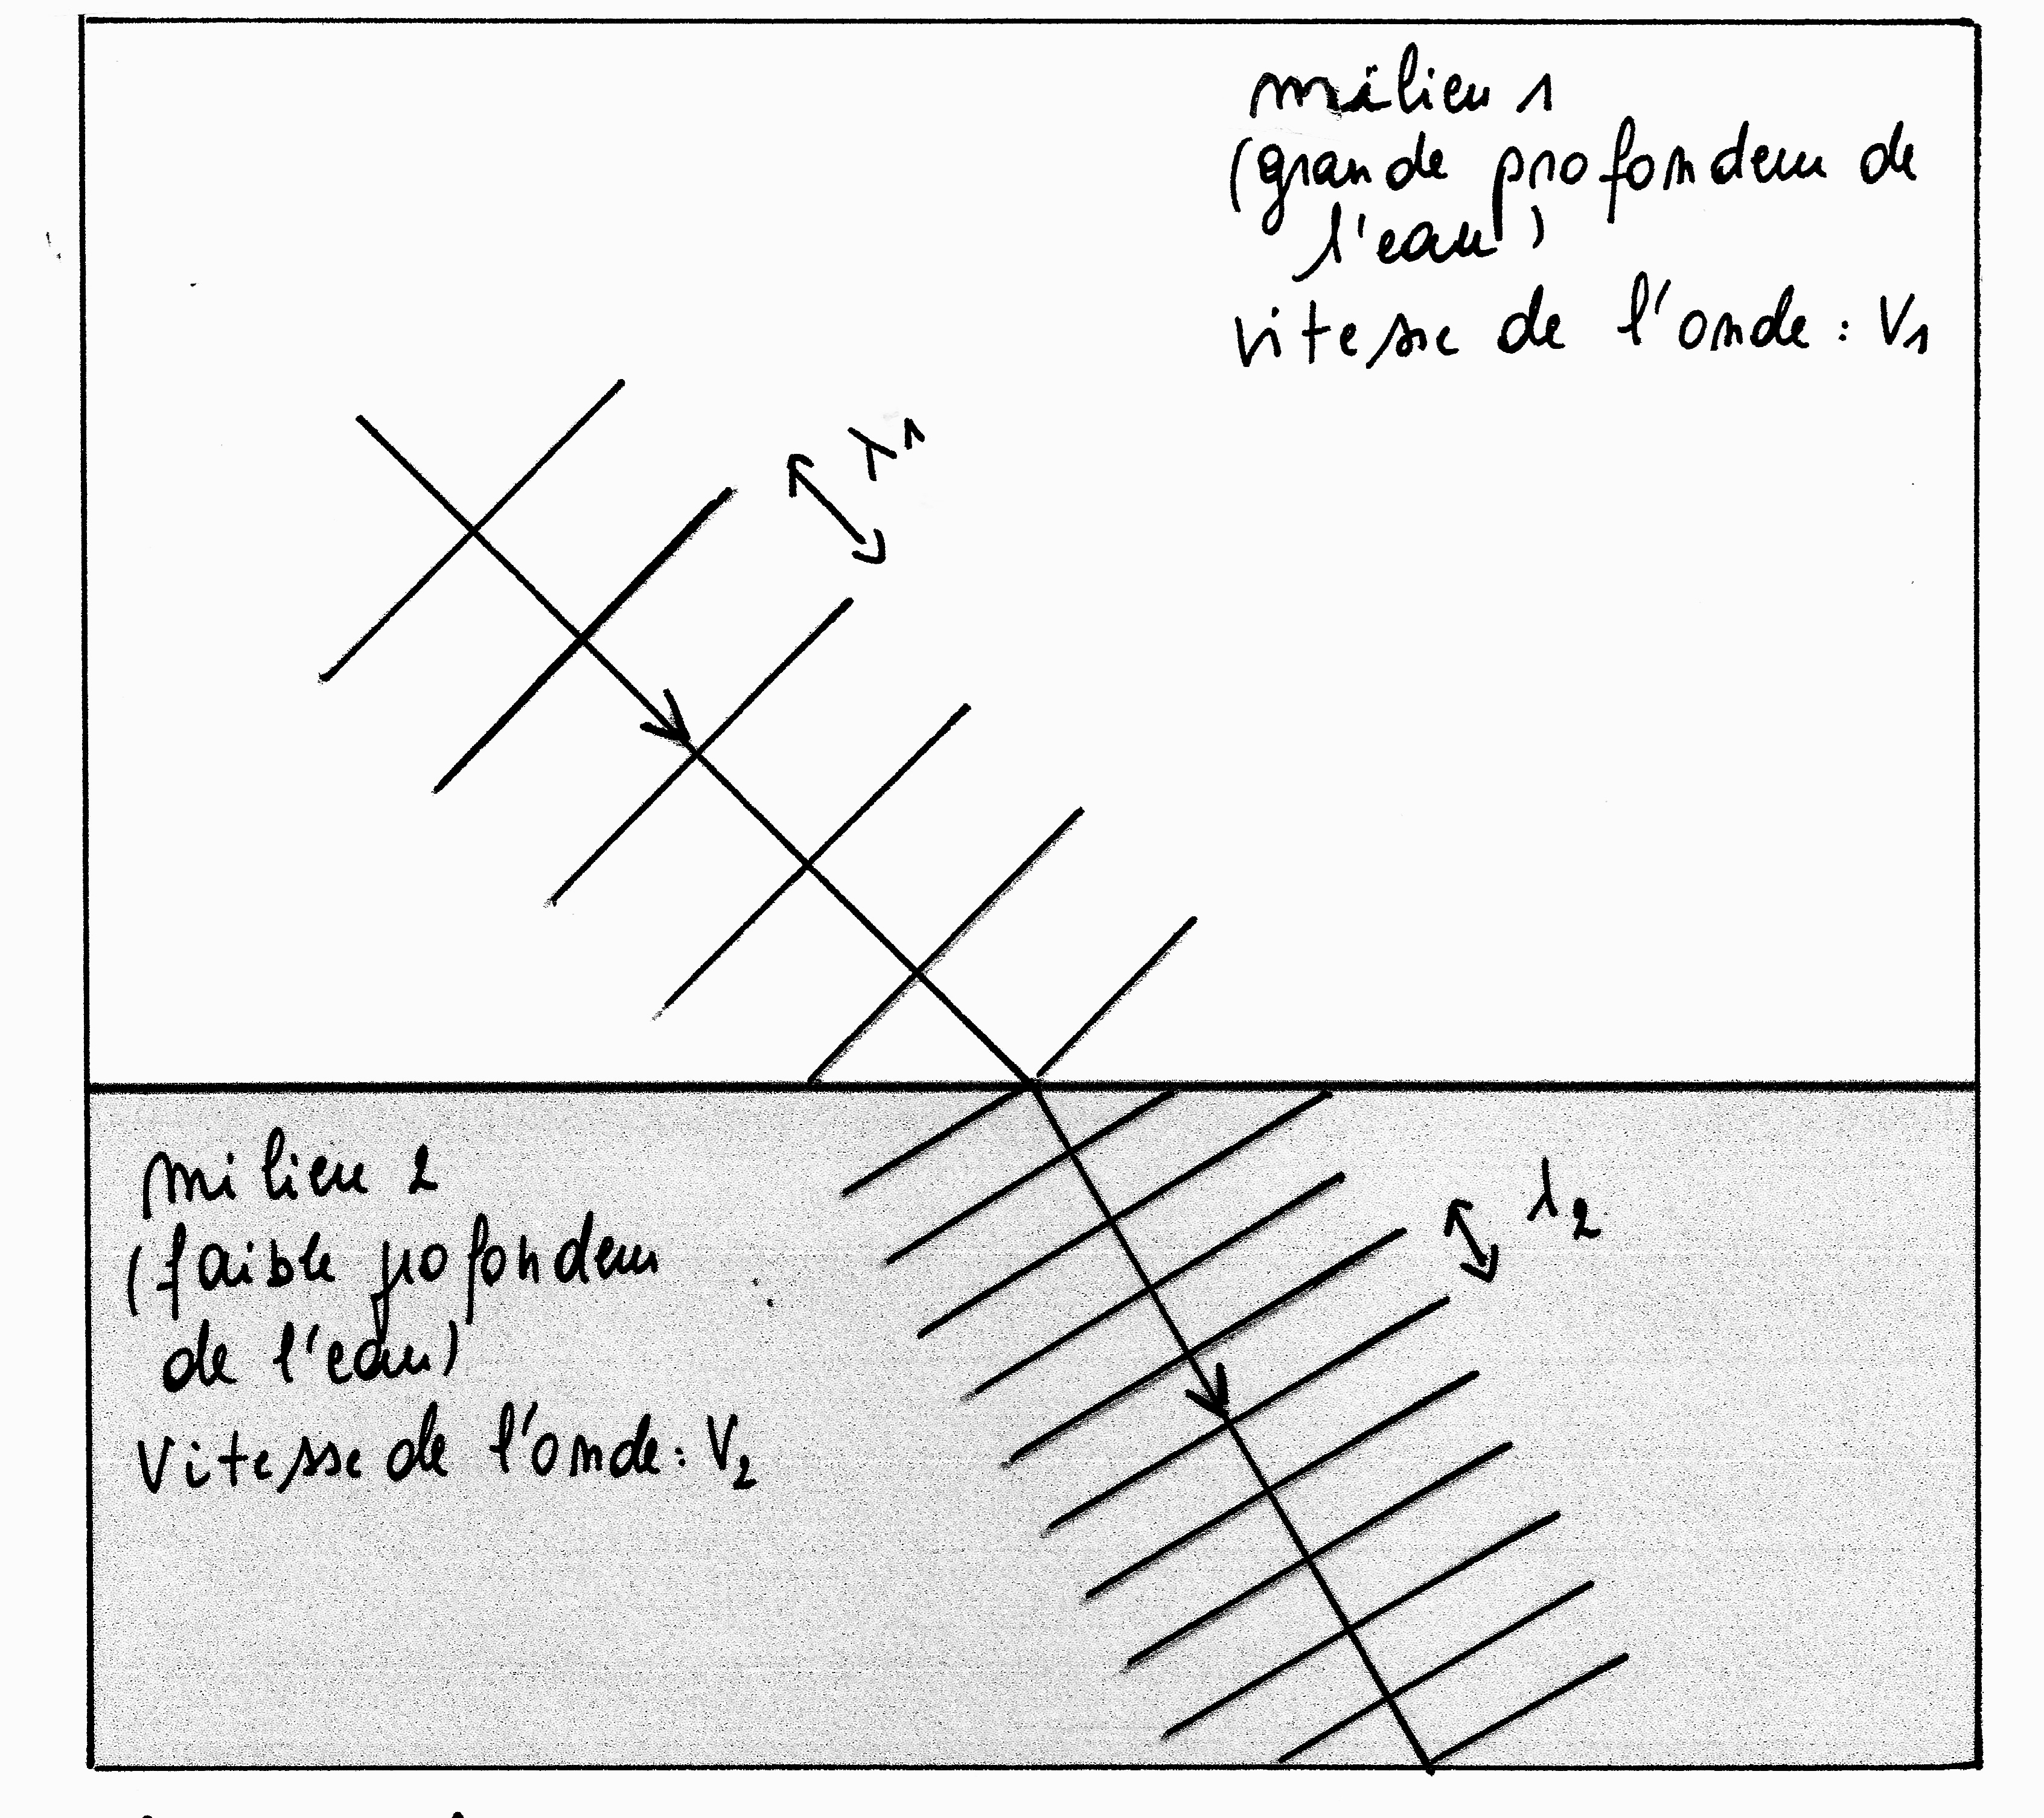
\includegraphics[width=5.076cm,height=4.512cm]{Pictures/1000000100000D3A00000BC4C32708B895F5FFB5.png}
\caption{}
\end{figure}

Comme l'onde passe d'un milieu profond à un milieu moins profond, elles
ralentissent et changent de direction.

Comment quantifier ce changement de direction~?

\begin{figure}
\centering
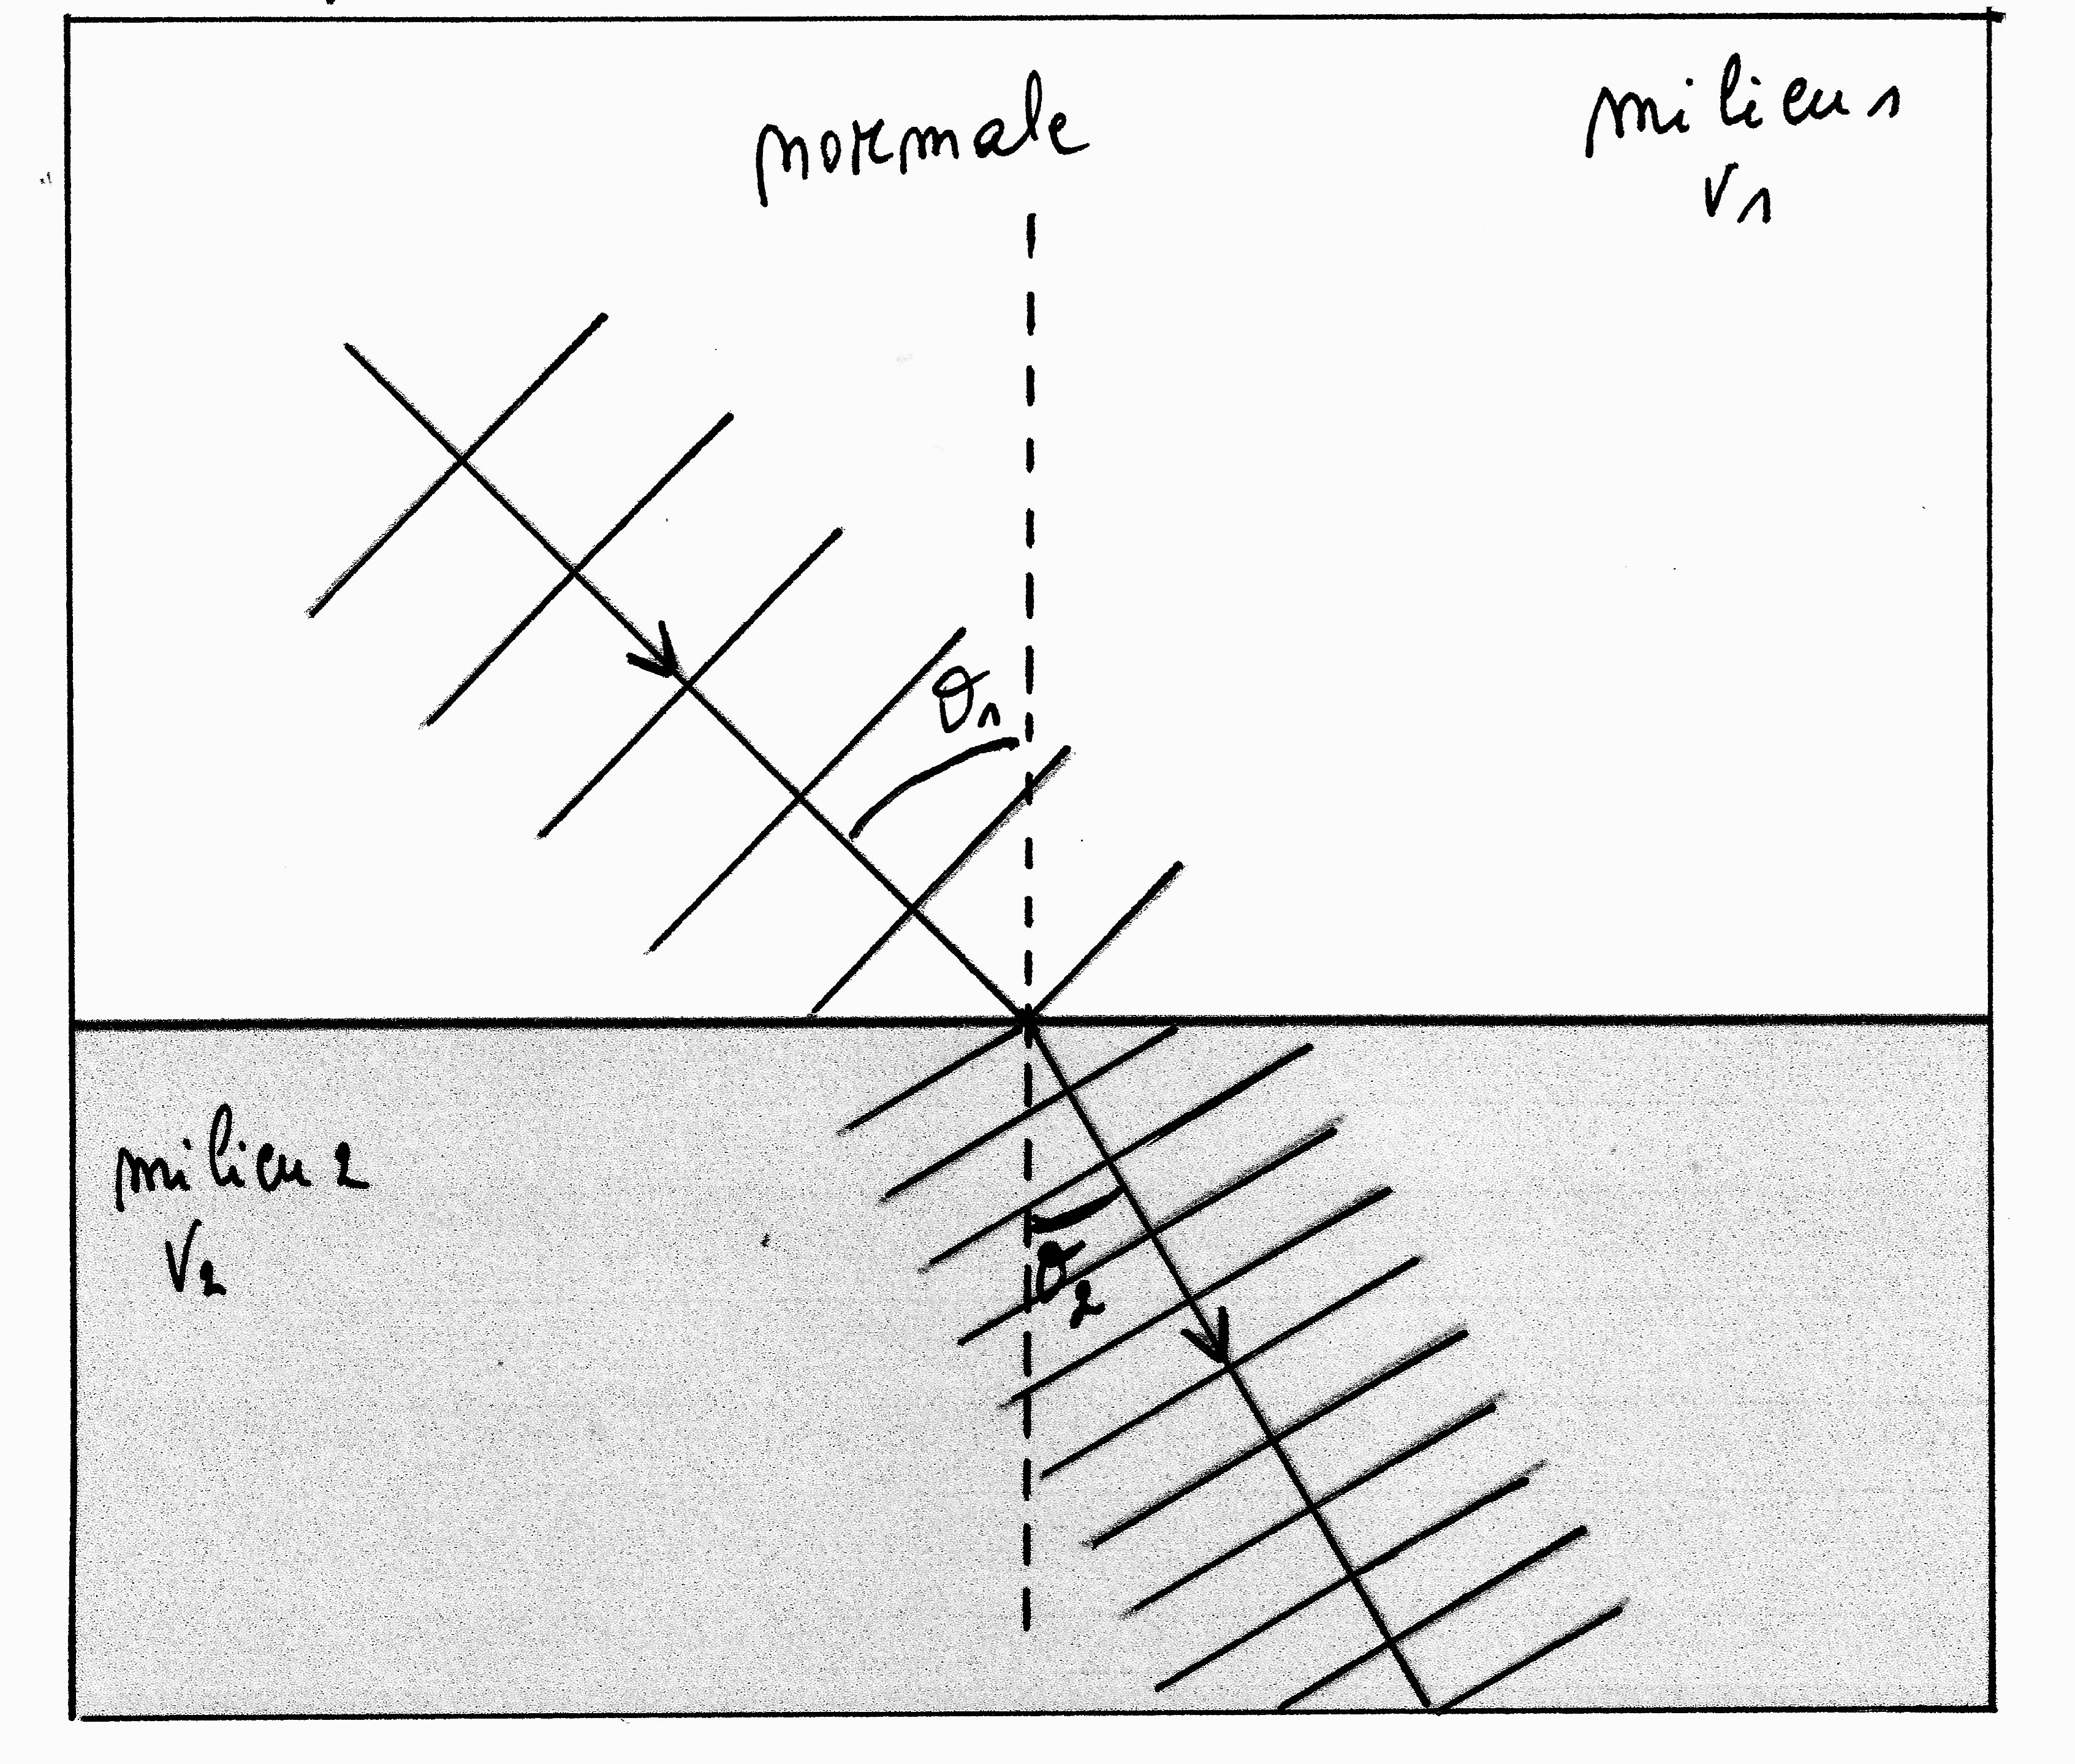
\includegraphics[width=6.652cm,height=5.652cm]{Pictures/1000000100000D3A00000B3EA693DF6AC5A29F0B.png}
\caption{}
\end{figure}

Définissons les angles d'incidence et de réfraction~:

a) \textbf{L'angle d'incidence (1)} est l'angle formé par la direction
de propagation de l'onde incidente et la normale (la perpendiculaire) à
l'obstacle.

b\textbf{) L'angle de réflexion (2)} est l'angle formé par la direction
des ondes réfractées et la normale.

Nous voyons ci-contre que~:

si $v_1 < v_2$ alors $\theta_1 >  \theta__2$ (l'onde se rapproche de la normale).
FIXME à vérifier

Quelle est la relation entre les vitesses et les angles d'incidence et
de réfraction~?

\begin{figure}
\centering
\includegraphics[width=18.516cm,height=20.461cm]{Pictures/10000001000013080000150A74E0EE61F2B1EE2F.png}
\caption{}
\end{figure}

\begin{figure}
\centering
\includegraphics[width=2.634cm,height=1.412cm]{Pictures/1000000100000045000000258E7A9DA5E900B5EA.png}
\caption{}
\end{figure}

\subsection{Applications de la réfraction}

On sait que le son se propage plus loin la nuit que le jour,
lorsqu'un son est produit au niveau du sol. Pourquoi cette différence~?

\includegraphics[width=8.356cm,height=5.151cm]{Pictures/100000010000021B0000014C687D75FBC118E240.png}

Durant
la journée, la température de l'air diminue quand on s'élève en
altitude. En effet, le sol chauffe plus rapidement que l'atmosphère.

Or, la vitesse du son diminue lorsque la température diminue.

Nous avons vu que lorsque la vitesse d'une onde diminue, l'onde se
réfracte de telle sorte que l'angle de réfraction r soit inférieur à
l'angle d'incidence i.

En traversant différentes couches d'air de plus en plus froides en
s'élevant, le son est dévié vers le haut. Un observateur au sol
n'entendra plus le son.

\begin{figure}
\centering
\includegraphics[width=8.414cm,height=5.172cm]{Pictures/1000000100000226000001526F2E95C895BB2EC1.png}
\caption{}
\end{figure}

Durant la nuit, le phénomène inverse se passe. La température de l'air
augmente quand on s'élève. En effet, le sol se refroidit plus vite que
l'atmosphère.

\textbf{La vitesse du son augmente lorsque la température augmente} et
donc la vitesse de l'onde réfractée est plus grande que la vitesse de
l'onde émise. L'angle de réfraction sera plus grand que l'angle
d'incidence et l'onde, étant réfractée vers le sol, se rapproche du sol
et le son porte plus loin.

\subsection{Exercice}

\subsubsection{Ex. 1}
\includegraphics[width=7.807cm,height=4.581cm]{Pictures/10000001000004570000028CCC770E758E0BAEF3.png}

Dans
le cadre d'un phénomène de réflexion~: quel est l'angle $\theta$ sur cette
figure~? ( Réponse~: 65°)

\subsubsection{Ex. 2 }
%( N° 6 du livre p 78)}}

\includegraphics[width=7.086cm,height=4.948cm]{Pictures/10000001000003620000025DC72F2F5C1B5B30DC.png}

La
figure ci-contre représente le passage d'une onde d'un milieu A vers un
milieu B.
\begin{enumerate}
	\item Dans lequel de ces deux milieux la vitesse de propagation est-elle la
	plus élevée~?
	\item  Si la fréquence des ondes est de 50 Hz et que la figure est à
	l'échelle 1:1, calculer la vitesse de l'onde dans chaque milieu.
\end{enumerate}

\subsubsection{Ex. 3}

Construire le schéma de réfraction d'une onde ayant une vitesse
incidente $v_1$ et une vitesse $v_2$ dans le second milieu, avec $v_1 =
1,5 v_2$} ; pour les angles d'incidence suivants :
\begin{enumerate}
	\item i = 10°
	\item i = 30 °
	\item i = 41,5 °
	\item i = 89°
\end{enumerate}

\subsubsection{Ex. 4}

Construire le schéma de réfraction d'une onde ayant une vitesse
incidente $v_1$ et une vitesse $v_2$ dans le second milieu, avec $v_2 =
2/3 v_1$ ; pour les angles d'incidence suivants :
\begin{enumerate}
	\item  i = 10°
	\item  i = 30 °
	\item  i = 41,5 °
	\item  Calculer l'angle limite de réfraction
	\item  Construire la propagation de l'onde pour un angle d'incidence i = 50
	°
\end{enumerate}

\subsubsection{Ex. 5} % (N°8 du livre p 78) 

Quel est l'angle d'incidence maximal pour qu'une onde sonore émise dans
l'air puisse être réfractée dans l'eau sans subir de réflexion totale à
la surface de l'eau ?

\subsubsection{Ex.  6} % ( N° 7 DU LIVRE P 78)

Dans un canal de navigation de 25 mètres de large, une onde; dont la
longueur d'onde est de 1,5 m,; se propage à la vitesse de 2 m/s. Que
devient cette longueur d'onde lorsque l'onde arrive dans une partie
moins profonde du canal où la vitesse de propagation est réduite à 1,6
m/s ?

\subsection{Résolutions}

\includegraphics[width=18.501cm,height=21.812cm]{Pictures/100000010000133200001AE8CBE600732ABF4D48.png}

\includegraphics[width=18.501cm,height=25.636cm]{Pictures/100000010000026D0000035C988B6F7E90298C6A.png}

\includegraphics[width=18.501cm,height=25.636cm]{Pictures/100000010000026D0000035C190239246DBF1AB2.png}

\includegraphics[width=18.501cm,height=25.636cm]{Pictures/100000010000026D0000035CCC97A4EC19D02B04.png}

\includegraphics[width=18.501cm,height=25.636cm]{Pictures/100000010000026D0000035CFF0F2F588EBA9209.png}

\includegraphics[width=18.501cm,height=25.527cm]{Pictures/1000000100000278000003689DDE3826ADE887B9.png}

\include{COURS_06-Diffraction_+_exercices(résolus).tex}
\section{Interférences}

Le phénomène d'interférence est du à la superposition de deux
ondes.

Il en résulte des zones où les ondes s'additionnent (zone de
tempête) et des zones où la superposition des ondes donne une amplitude
résultante nulle (zone de repos).

\includegraphics[width=8.326cm,height=3.881cm]{Pictures/10000001000001A4000000C3DDA5D7BD0B699726.png}

\subsection{Expérience avec la cuve à onde}

FIXME ajouter des descriptions d'expériences avec la cuve à ondes

Nous avons visualisé ce phénomène à l'aide de la cuve à ondes.

Pour ce faire, nous avons pris des pointes qui vibrent dans l'eau,
chacune produisant des ondes circulaires.

Nous avons obervé des endroits où l'eau est en mouvement et des endroits
où l'eau est au repos. Comment expliquer cette observation?

\subsubsection{Analyse théorique}

Prenons deux sources $S_1$ et $S_2$ émettant
en concordance de phase des ondes de même fréquence (on dira que les
sources sont alors \emph{cohérentes}).

\begin{figure}
\centering
\includegraphics[width=8.47cm,height=8.927cm]{Pictures/10000001000001DE000001F885F9EB969C92123B.png}
\caption{}
\end{figure}

Les cercles concentriques représentent les vagues vues de haut
\emph{(les cercles en traits pleins des crètes et les cercles en traits
pointillés des creux).}

Nous voyons bien que les 2 sources ($S_{1}$ et
$S__{2}$) émettent des ondes de même longueur d'onde et donc
de même fréquence.

Considérons le point M. 

L'onde produite par $S_1$ a parcouru une distance
$d_1$ pour arriver en M et l'onde produite par
$S_2$ a parcouru une distance $d_2$ pour
arriver en M. Les deux ondes arrivent donc au point M avec un déphasage
puisqu'elle n'ont pas parcouru la même distance.

Dans notre exemple ci-contre :
\begin{enumerate}
	\item La distance $d_1$ parcourue par l'onde provenant de
	$S_1$ jusque M est égale à $3 \cdot \frac{1}{2}$ (trois demi-longueur
	d'onde). Regardez sur le schéma.
	\item La distance $d_2$ parcourue par l'onde provenant de
	$S_2$} jusque M est égale à $4 \cdot \frac{1}{2}$(quatre demi-longueur
	d'onde).
	\item  Les deux ondes arrivent donc en M décalées de $\frac{4}{2} - \frac{3}{2} = \frac{1}{2} $
\end{enumerate}

Elles sont donc au point M en opposition de phase l'une par rapport à
l'autre. En effet, au point M, l'onde provenant de $S_1$
est une crète tandis que l'onde provenant de $S_2$ est un
creux. Donc, au point M, l'eau sera au repos. On parlera
\emph{d'interférence destructive.}

Nous appelerons \textbf{$d_2 - d_1 = \Delta_{12}, \emph{la différence de
marche.}

\includegraphics[width=9.596cm,height=10.112cm]{Pictures/10000001000001DE000001F885F9EB969C92123B.png}

Considérons le point N. 

L'onde produite par $S_1$ a parcouru une distance
d\textsubscript{1} pour arriver en N et l'onde produite par
$S_2$ a parcouru une distance d\textsubscript{2} pour
arriver en N. Les deux ondes arrivent donc au point M avec un déphasage.
\begin{enumerate}
	\item La distance $d_1$ parcourue par l'onde provenant de
	$S_1$ jusque M est égale à $5 \frac{1}{2}$ (cinq demi-longueur
	d'onde). Regardez sur le schéma.
	\item La distance $d_2$ parcourue par l'onde provenant de
	$S_2$ jusque N est égale à $75 \frac{1}{2}$ (sept demi-longueur
	d'onde).
	\item Les deux ondes arrivent donc en M décalées de ($\frac{7}{2} - \frac{5}{2} =  \frac{2}{2}$ longueur d'ondes.
\end{enumerate}

Elles sont donc au point N en concordance de phase l'une par rapport à
l'autre. En effet, au point N, l'onde provenant de $S_1$
est une crète et de même, l'onde provenant de $S_2$ est une
crète. Donc, au point N, deux crètes vont se superposer, ce qui donnera
de l'eau en mouvement avec une amplitude double par rapport aux
amplitudes des sources. On parlera \emph{d'interférence
constructive.}

\subsection{Représentations}
\includegraphics[width=7.264cm,height=8.423cm]{Pictures/100000010000021B000002719784CD0CAF081F55.png}

\subsubsection{Hyperboles de repos et hyperboles de tempête}

Pour expliquer les zones de tempête et de repos, observez attentivement
le schéma ci-contre :
\begin{enumerate}
	\item En chaque point d : chaque point d est atteint par un creux (cercle en pointillé)
	et une crète (cercle en trait plein), la résultante du
	mouvement nous donne donc une \textbf{zone de repos.} Vous pouvez ainsi
	observer ces courbes (ce sont des hyperboles) où l'eau au repos.
    \itemEn chaque point c : Chaque point c est atteint par soit deux creux (cercles en pointillé, soit deux crètes (cercles en trait plein), la résultante du mouvement nous donne donc une \textbf{zone de tempête.} Vous pouvez ainsi observer ces courbes (ce sont des hyperboles) où l'eau est en mouvement.
\end{enumerate}

\begin{figure}
\centering
\includegraphics[width=13.005cm,height=3.542cm]{Pictures/1000000100000220000000A31734CD7DA5F285B4.png}
\caption{}
\end{figure}

\subsection{Exercices}

\subsubsection{Ex. 1}

Soient deux sources sonores ponctuelles S1 et S2. Elles envoient des
ondes en concordance de phase, dont la fréquence est égale à 5 Hz et qui
se propagent à la vitesse de 10 cm/s. L'amplitude de chacune des ondes
est de 3cm

Calculez l'amplitude d'un point P situé à 6 cm de S1 et à 8 cm de S2~?

\subsubsection{Ex. 2}

Deux haut-parleurs séparés de 2 m émettent un signal à 680 Hz en phase.
Un microphone est placé à 6,75 m de l'un et à 7 m de l'autre. Quelle est
l'amplitude du signal mesuré~?

\subsubsection{Ex. 3}

\begin{figure}
\centering
\includegraphics[width=5.151cm,height=2.729cm]{Pictures/10000001000000BC000000630AF71C86AA2A0A65.png}
\caption{}
\end{figure}

Deux haut-parleurs S1 et S2 distants de 6 m émettent des

ondes sonores en concordance de phase. Le point P de la

figure est à 8 m de S1. Quelle est la fréquence minimale
à laquelle l'intensité en P est~:

\begin{enumerate}
\item nulle~?
\item  maximale~?
\end{enumerate}

\subsubsection{Ex. 4}

\includegraphics[width=9.146cm,height=5.973cm]{Pictures/100000010000062500000404B4675BF2C4CE1EEC.png}Deux
petits haut-parleurs distants de 3 mètres émettent des sons de fréquence
constante de 344 Hz dans une pièce surchauffée. On déplace un microphone
P le long d'une droite parallèle à la ligne S1S2 joignant les deux
haut-parleurs et située à 4 mètres de cette ligne. On trouve deux maxima
d'intensité~: le premier au point O, équidistants des deux haut-parleurs
et le second juste en face de l'un d'eux.

Utilisant ces données, calculer la vitesse du son dans cette pièce
surchauffée

( rappel~: la vitesse du son dans l'air est de 340 m/s à une température
de 20°C)

\emph{\textbf{EXERCICE 5}}

\includegraphics[width=11.546cm,height=4.688cm]{Pictures/1000000100000363000001603D3E7105AB252F90.png}Les
deux haut-parleurs montrés sur la figure émettent, en phase, un son
ayant une longueur d'onde de 25 cm. Quelle est la distance minimale d
entre les haut-parleurs qu'il doit y avoir pour qu'il y ait de
l'interférence destructive pour l'observateur?

\emph{\textbf{EXERCICE 6}}

\begin{figure}
\centering
\includegraphics[width=4.757cm,height=7.147cm]{Pictures/10000001000001BA00000298E2F6E319C348E061.png}
\caption{}
\end{figure}

Les haut-parleurs de la figure émettent des ondes sonores en concordance
de phase. Quelle est la fréquence minimale qui permet d'obtenir de
l'interférence destructive à l'endroit où est situé l'observateur?

\emph{\textbf{INTERFERENCES - EXERCICES}}

\emph{\textbf{EXERCICE 1}}

Soient deux sources sonores ponctuelles S1 et S2. Elles envoient des
ondes en concordance de phase, dont la fréquence est égale à 5 Hz et qui
se propagent à la vitesse de 10 cm/s. L'amplitude de chacune des ondes
est de 3cm

Calculez l'amplitude d'un point P situé à 6 cm de S1 et à 8 cm de S2~?

\emph{\textbf{EXERCICE 2}}

Deux haut-parleurs séparés de 2 m émettent un signal à 680 Hz en phase.
Un microphone est placé à 6,75 m de l'un et à 7 m de l'autre. Quelle est
l'amplitude du signal mesuré~?

\emph{\textbf{EXERCICE 3}}

\begin{figure}
\centering
\includegraphics[width=5.151cm,height=2.729cm]{Pictures/10000001000000BC000000630AF71C86AA2A0A65.png}
\caption{}
\end{figure}

Deux haut-parleurs S1 et S2 distants de 6 m émettent des

ondes sonores en concordance de phase. Le point P de la

figure est à 8 m de S1. Quelle est la fréquence minimale

à laquelle l'intensité en P est~:

\begin{enumerate}
\def\labelenumi{\alph{enumi})}
\tightlist
\item
  nulle~?
\end{enumerate}

\begin{enumerate}
\def\labelenumi{\alph{enumi})}
\tightlist
\item
  maximale~?
\end{enumerate}

\emph{\textbf{EXERCICE 4}}

Deux petits haut-parleurs distants de 3 mètres émettent des sons de
fréquence constante de 344 Hz dans une pièce surchauffée. On déplace un
microphone P le long d'une droite parallèle à la ligne S1S2 joignant les
deux haut-parleurs et située à 4 mètres de cette ligne. On trouve deux
maxima d'intensité~: le premier au point O, équidistants des deux
haut-parleurs et le second juste en face de l'un d'eux.

Utilisant ces données, calculer la vitesse du son dans cette pièce
surchauffée

( rappel~: la vitesse du son dans l'air est de 340 m/s à une température
de 20°C)

\begin{figure}
\centering
\includegraphics[width=15.663cm,height=10.231cm]{Pictures/100000010000062500000404B4675BF2C4CE1EEC.png}
\caption{}
\end{figure}

\emph{\textbf{EXERCICE 5}}

\includegraphics[width=11.546cm,height=4.688cm]{Pictures/1000000100000363000001603D3E7105AB252F90.png}Les
deux haut-parleurs montrés sur la figure émettent, en phase, un son
ayant une longueur d'onde de 25 cm. Quelle est la distance minimale d
entre les haut-parleurs qu'il doit y avoir pour qu'il y ait de
l'interférence destructive pour l'observateur?

\includegraphics[width=4.757cm,height=7.147cm]{Pictures/10000001000001BA00000298E2F6E319C348E061.png}\emph{\textbf{EXERCICE
6}}

Les haut-parleurs de la figure émettent des ondes sonores en phase.
Quelle est la fréquence minimale qui permet d'obtenir de l'interférence
destructive à l'endroit où est situé l'observateur?

\includegraphics[width=18.253cm,height=25.273cm]{Pictures/100000010000027000000360A2E9B52B5C1C825B.png}

\includegraphics[width=18.253cm,height=25.273cm]{Pictures/100000010000027000000360F8FFC5B3763173F1.png}

\includegraphics[width=18.253cm,height=25.273cm]{Pictures/100000010000027000000360FFD6C2C9381DA208.png}

\includegraphics[width=18.253cm,height=25.273cm]{Pictures/1000000100000270000003604BA27A8CAE787E63.png}


\section{Effet Doppler}
\label{effet-doppler}

\subsection{Mise en situation}

\begin{figure}
\centering
\includegraphics[width=8.557cm,height=4.856cm]{Pictures/1000000100000162000000C9EFEF725F14698266.png}
\caption{}
\end{figure}

Lorsqu'une source d'ondes sonores se déplace, on observe que la
fréquence du son entendu est différente du son qu'on entendrait si la
source est immobile.

Par exemple, lorsque la sirène d'une ambulance ou d'une voiture de
police s'approche d'un auditeur, le son perçu par l'auditeur est plus
aigu (fréquence plus élevée).

Lorsque la sirène d'une ambulance ou d'une voiture de police s'éloigne
d'un auditeur, le son perçu par l'auditeur est plus grave (fréquence
plus basse).

Il y a également un changement de fréquence si l'observateur est en
mouvement et la source est immobile. Le son est plus aigu quand on se
dirige vers la source et plus grave quand on s'éloigne de la source.

Ce changement de fréquence du au mouvement de l'observateur ou de la
source porte le nom d'effet Doppler puisque la théorie décrivant cet
effet fut développée par le physicien allemand Christian Doppler en
1842.

\subsection{Étude quantitative}

Trois situations peuvent être traitées~:
\begin{enumerate}
	\item L'observateur s'éloigne ou se rapproche de la source fixe.
	\item La source s'éloigne ou se rapproche d'un observateur fixe.
	\item La source et l'observateur bougent successivement l'un par rapport à l'autre.
\end{enumerate}

Nous supposerons pour chacune des situations que l'observateur ou la
source se déplace suivant une trajectoire rectiligne et à vitesse
constante.

La différence de fréquence entre celle émise et celle perçue est due à
une variation de la longueur d'onde perçue par l'observateur.

\begin{figure}
\centering
\includegraphics[width=16.611cm,height=7.362cm]{Pictures/1000000100000234000000FA4BFBBF5E6B58FB9F.png}
\caption{}
\end{figure}

\subsection{Une source en mouvement s'approche de l'observateur fixe à une vitesse $v_s$}

Nous noterons~:
\begin{enumerate}
	\item $v_s$~: la vitesse de la source
	\item $v$~: la vitesse de l'onde.
	\item $f$~: la fréquence émise par la source
\end{enumerate}

\includegraphics[width=17.231cm,height=24.262cm]{Pictures/10000001000002390000032125422D51A14758E6.png}\textbf{f
`~: la fréquence perçue par l'observateur. }

Nous pourrions dans le même état d'esprit, démontrer les relations entre
$f$ et $f'$ pour les autres situations~:
\begin{enumerate}
	\item L'observateur s'éloigne ou se rapproche de la source fixe.
	\item La source s'éloigne d'un observateur fixe.
\end{enumerate}

Je vous laisse le plaisir de les réaliser.

En résumé, voici les relations pour les 4 situations~:
\begin{figure}
\centering
\includegraphics[width=17.866cm,height=17.32cm]{Pictures/100000010000025C00000234BE3EA55298C88B1D.png}
\caption{}
\end{figure}

\subsection{Exercices}

\subsubsection{Exercice 1}% (N°14 du livre p 79)

La fréquence d'une sirène est de 600 Hz (perception au repos).

Si un observateur perçoit ces ondes avec une fréquence de 580 Hz, y
a-t-il éloignement ou rapprochement entre lui et la sirène~?

\subsubsection{Exercice 2} %(N°18 du livre p 80)

La sirène d'une voiture de police a une fréquence de 1200 Hz. Quelle est
la fréquence entendue par un observateur immobile si la voiture se
déplace à 108 km/h~:
\begin{enumerate}
	\item vers l'observateur~?
	\item en s'éloignant de l'observateur~?
\end{enumerate}

\subsubsection{Exercice 3} %(N°19 du livre p 80)

Une source sonore émet à une fréquence de 600 Hz. Ce signal est perçu par
un observateur immobile avec une fréquence de 640 Hz lorsque la source
s'approche de lui. Calculer la fréquence perçue si la source s'éloigne à
la même vitesse.

\subsubsection{Exercice 4} % (N°20 du livre p 80)

La sirène d'une voiture de police a une fréquence de 600 Hz. La voiture
s'approche d'un grand mur à la vitesse de 108 km/h. Calculer la
fréquence du son réfléchi entendu par le policier dans la voiture.

\subsubsection{Exercice 5} % (N°21 du livre p 80)

Debout sur le trottoir, un piéton perçoit une fréquence de 510 Hz
provenant de la sirène d'une voiture de police qui s'approche. Après le
passage de la voiture, la fréquence perçue du son de la sirène par le
piéton est de 430Hz. Calculer la vitesse de la voiture.

\subsubsection{Exercice 6 }

\includegraphics[width=7.4cm,height=3.882cm]{Pictures/10000001000001A1000000DB0C45621DF12277A1.png}
Simone, conducteur d'une auto, fait fonctionner son klaxon, qui a une fréquence de
350 Hz, pour prévenir Albert qui est distrait sur la rue.
\begin{enumerate}
	\item Quelle est la fréquence du son entendu par Albert?
	\item Quelle est la longueur d'onde du son perçu par Albert?
	\item Quelle est la fréquence du son entendu par Simone~?
	\item Quelle est la longueur d'onde du son perçu par Simone~?
\end{enumerate}

(Rép~: 390 Hz~; 87 cm~; 317 Hz~; 1,07 m)

\subsubsection{Exercice 7}

La raie spectrale de l'hydrogène ayant normalement une longueur d'onde
de 656,279 nm a une longueur d'onde de 656,263 nm dans le spectre de
l'étoile Sirius observé sur la Terre. À quelle vitesse Sirius
s'approche-t-elle ou s'éloigne-t-elle de nous?

(Rép~:7314 m/s)

\subsection{Résolutions}

FIXME à faire
\section{Expériences de Young}}

FIXME ajouter biographie de Thomas Young

\subsection{Mise en évidence du comportement ondulatoire de la
lumière.}

\subsubsection{Interférences d'un son (onde sonore)}

\includegraphics[width=7.922cm,height=3.875cm]{Pictures/1000000100000156000000A71108C5553D5F186E.png}

\paragraph{Exemple 1}

Deux haut-parleurs sont distants de 1 mètre et émettent chacun un son
d'une fréquence égale à 1000 Hz en concordance de phase.

Comment sera l'intensité du son perçu au point P ?

\begin{figure}
\centering
\includegraphics[width=4.12cm,height=2.434cm]{Pictures/100000010000009E0000005DF543EBD570977663.png}
\caption{}
\end{figure}

Réponse~:
P est situé en un point tel que $S_1$= 
la différence de marche $d_{2} - d_{1}$ est
nulle et donc les ondes arrivent au point P en concordance de phase. Il
s'agit d'un point d'interférence constructive et l'intensité du son en P
sera maximale.

\begin{figure}
\centering
\includegraphics[width=7.154cm,height=4.233cm]{Pictures/1000000100000197000000F1DA056A96FDEF75DB.png}
\caption{}
\end{figure}

\paragraph{Exemple 2}

Deux haut-parleurs sont distants de 1 mètre et émettent chacun un son
d'une fréquence égale à 1000 Hz en concordance de phase.

Comment sera l'intensité du son perçu au point P1 si ce point se trouve
à une distance i=1,36 m du point P?

\begin{figure}
\centering
\includegraphics[width=15.545cm,height=11.171cm]{Pictures/100000010000025F000001BE110A2F11D2815100.png}
\caption{}
\end{figure}

\subsubsection{Généralisation}

\includegraphics[width=7.086cm,height=5.068cm]{Pictures/10000001000001CB00000148F2D7DB2B0F2EC580.png}

Nous
voyons donc que lorsque nous nous déplaçons sur la droite verticale (que
nous appellerons l'écran), nous parcourons une succession de zones
d'interférences constructives (IC) et d'interférences destructives (ID).

Les zones d'interférences constructives sont telles que l'intensité du
son est maximale et les zones d'interférences destructives, telles que
l'intensité du son est nulle. Elles sont séparées d'une distance i
(appelée interfrange)

\includegraphics[width=8.123cm,height=5.352cm]{Pictures/100000010000018B00000104CBB3B40EFC3646D7.png}

La question est~: pouvons-nous trouver la distance qui sépare les zones
d'interférence constructives (l'interfrange $i$), en fonction de
$\delta$, a et d où~: 

\begin{description}
 \item{\delta}~: longueur d'onde des sons émis.
 \item{i}~: distance entre deux zones d'interférences constructives.
 \item{d}~: distance entre les sources et l'écran.
 \item{a}~: distance entre les deux sources.
\end{description}

Remarquez sur le schéma ci-contre~: $x_{1}=i$,
$x_{2}-x_{1} = i$,
$x_{3}-x_{2} = i$, \ldots.

$x$ est la distance entre le point central et un point d'interférence
constructive.

\begin{figure}
\centering
\includegraphics[width=17.253cm,height=13.09cm]{Pictures/100000010000025F000001F704069EFE234008BD.png}
\caption{}
\end{figure}

\subsubsection{Interférence lumineuse }

\paragraph{Expérience de Young~: diffraction à travers deux fentes
et figure d'interférences. }

Nous venons de voir que les interférences sonores sont caractéristiques
d'un comportement ondulatoire.

\includegraphics[width=10.592cm,height=6.443cm]{Pictures/100000010000025A000001696E99605075C8F3D0.png}\emph{\textbf{Que
se passera-t-il si nous soumettons la lumière à cette expérience
d'interférence~? }}

Décrivons cette expérience, \emph{\textbf{l'expérience de Young.}}

De la lumière provenant d'un laser traverse un écran percé de deux
fentes fines, distantes d'une courte distance a (les fentes de Young).

Sur un écran, situé à une distance D des fentes, on observe une
succession de points lumineux, séparés par une distance i.

\begin{figure}
\centering
\includegraphics[width=8.299cm,height=7.35cm]{Pictures/10000001000001410000011C9E9E805F9A9605B7.png}
\caption{}
\end{figure}

\emph{Interprétation }

En analogie avec deux sources d'ondes sonores, nous pouvons conclure que
seul le modèle ondulatoire peut expliquer ces observations.

Les deux fentes de Young S1 et S2 vont se comporter comme de nouvelles
sources et diffracter la lumière incidente provenant du laser.

Ces deux ondes vont produire des interférences sur l'écran et produire
une succession de points lumineux.

Les points lumineux sont des zones d'interférences constructives et
entre les points lumineux, l'absence de lumière, correspond à des zones
d'interférences destructives, ce qui est typiquement un comportement
ondulatoire.

Nous avons démontré précédemment, dans le cas d'interférences de deux
ondes sonores, le lien qui relie , i, a et D. En suivant une démarche
identique pour cette expérience de Young, nous obtenons la relation~:

\begin{figure}
\centering
\includegraphics[width=1.788cm,height=1.46cm]{Pictures/100000010000001A00000015860A63C6525557ED.png}
\caption{}
\end{figure}

Dans notre situation~: i et a sont très petits devant D, l'approximation
est très pertinente (voir démonstration).

L'expérience de Young avec de la lumière conduit à la même relation~:

\emph{\textbf{Cette expérience montre que la lumière a un caractère
ondulatoire et donc que la lumière}}

\emph{\textbf{se comporte comme une onde. Elle est donc caractérisée par
une fréquence f et une longueur d'onde }\textbf{}\textbf{.}}

\emph{\textbf{b) }\textbf{Calcul angulaire de la position des points
d'interférence constructive}}

\begin{figure}
\centering
\includegraphics[width=7.071cm,height=5.604cm]{Pictures/10000001000001D8000001766572F750E44C7125.png}
\caption{}
\end{figure}

Soit P\textsubscript{1}, un point d'interférence constructive situé
juste après le point central, notons θ la position angulaire de ce
point.

En ce point P\textsubscript{1}, l'interférence étant constructive, la
différence de marche d= d\textsubscript{2} -- $S_1$ =


En faisant l'approximation déjà réalisée précédemment, à savoir~: a et i
 D, nous pouvons considérer que les rayons lumineux d1 et d2 sont
quasiment parallèles.

En considérant le triangle rectangle représenté sur le schéma~:

d= = a Sin θ

\begin{figure}
\centering
\includegraphics[width=2.095cm,height=1.107cm]{Pictures/100000010000002800000015DDF3AE193165C3E3.png}
\caption{}
\end{figure}

Nous avons donc que~:  = a Sin θ et donc~:

\includegraphics[width=5.061cm,height=4.096cm]{Pictures/10000001000001D80000017E98931F1CF545D918.png}\emph{\textbf{Généralisation
}}

- Considérons un point P\textsubscript{2}

En ce point P\textsubscript{2 }, l'interférence étant constructive, la
différence de marche d= d\textsubscript{2} -- $S_1$ =
2

En considérant le triangle rectangle représenté sur le schéma~: d= =
a Sin θ

Donc~:
\includegraphics[width=2.306cm,height=1.107cm]{Pictures/100000010000002C000000153ADDDC592928E9B8.png}

En continuant le raisonnement de la sorte pour des points~:

P\textsubscript{3} distant de 3i du point central,

P\textsubscript{4} distant de 4i du point central,

P\textsubscript{5} distant de 5i du point central, \ldots{}

\begin{figure}
\centering
\includegraphics[width=2.306cm,height=1.107cm]{Pictures/100000010000002C0000001558E0CCA95D4F59EB.png}
\caption{}
\end{figure}

Nous arrivons à~:

\includegraphics[width=7.086cm,height=5.897cm]{Pictures/100000010000020C000001B4676C159EC881E6E3.png}\emph{\textbf{Synthèse:}}

\begin{figure}
\centering
\includegraphics[width=1.757cm,height=1.432cm]{Pictures/100000010000001A000000159D382765312EA964.png}
\caption{}
\end{figure}

\begin{figure}
\centering
\includegraphics[width=2.894cm,height=1.389cm]{Pictures/100000010000002C0000001558E0CCA95D4F59EB.png}
\caption{}
\end{figure}

\emph{\textbf{4)Applications}}

\emph{\textbf{3.1 Détermination expérimentale de la longueur d'onde de
la lumière. }}

L'expérience de Young permet de déterminer la fréquence de la lumière

a) Réalisons l'expérience de Young avec une lumière jaune et les données
suivantes~:

D=1,75 m

a=1 mm

i~=1 mm

\includegraphics[width=16.82cm,height=5.733cm]{Pictures/1000000100000243000000D01464CBCF0F7AAEC1.png}Calculez
la longueur d'onde de la lumière jaune ainsi que la fréquence de la
lumière correspondante.

b)\textbf{ }Réalisons l'expérience de Young avec une lumière verte
sachant que l'expérience de Young nous fournit les valeurs suivantes~:

D=4,95 m

a=0,2 mm

i~=1,32 cm

Calculez la longueur d'onde de la lumière verte ainsi que la fréquence
de la lumière correspondante. Exprimez votre réponse en nm.

\begin{figure}
\centering
\includegraphics[width=15.833cm,height=8.654cm]{Pictures/100000010000023700000151168D50BCCC321003.png}
\caption{}
\end{figure}

\emph{\textbf{c) Le spectre de la lumière blanche}}

\emph{\textbf{Ces expériences nous montrent que chaque couleur de la
lumière possède une longueur d'onde et donc une fréquence
caractéristique de la couleur. }}

\textbf{}\textsubscript{\textbf{jaune}}\textbf{ 
}\textsubscript{\textbf{vert}}\textbf{ et donc
f}\textsubscript{\textbf{jaune}}\textbf{ 
f}\textsubscript{\textbf{vert}}

Or la lumière blanche est composée de toutes les couleurs de l'arc en
ciel. L'expérience de Young nous permet donc de classer toutes les
couleurs qui composent la lumière blanche en fonction de leur longueur
d'onde ( et donc de leur fréquence).

C'est ce qu'on appelle \emph{\textbf{le spectre de la lumière blanche.
(voir livre p 115)}}

\begin{figure}
\centering
\includegraphics[width=11.557cm,height=5.907cm]{Pictures/1000000100000186000000C7B42157D8D8096212.png}
\caption{}
\end{figure}

\includegraphics[width=9.176cm,height=6.676cm]{Pictures/10000001000001FB0000017167AEF9D1A02E0A78.png}\emph{\textbf{d)
Diffraction de la lumière blanche}}

Si on réalise l'expérience de diffraction de la lumière blanche par un
réseau, on observe que chaque couleur présentera ses maximums à un angle
différent, sauf pour le maximum central qui est à la même position (θ =
0) pour toutes les couleurs.

\includegraphics[width=2.259cm,height=1.082cm]{Pictures/100000010000002C0000001558E0CCA95D4F59EB.png}Les
plus grandes longueurs d'onde subiront les plus grandes déviations.

\textbf{Le maximum d'ordre 1 du mauve sera celui le plus près du
maximum} central puisque c'est la longueur d'onde visible la plus petite
alors que \textbf{le maximum d'ordre 1 le plus éloigné du maximum
central sera celui du rouge} puisque c'est cette couleur du visible qui
a la plus grande longueur d'onde. On aura alors la figure d'interférence
ci-contre.

\emph{\textbf{Applications~: }}

Les plumes si colorées de certains oiseaux.

\emph{\textbf{EXERCICES}}

\hypertarget{exercice-1}{%
\section{\texorpdfstring{\emph{Exercice
1}}{Exercice 1}}\label{exercice-1}}

De la lumière de longueur d'onde égale à 600 nm éclaire, suivant la
normale, deux fentes séparées de 0,1 mm.

\begin{enumerate}
\def\labelenumi{\alph{enumi})}
\tightlist
\item
  Quelle est la position angulaire d'ordre 1? (Rép~: 0,34°)
\item
  A quelle distance du point central se trouve ce maximum d'ordre 1~sur
  un écran situé à 3 mètres des fentes? (Rép~: 18 mm)
\end{enumerate}

\begin{quote}
\emph{\textbf{Exercice 2}}
\end{quote}

\begin{quote}
\end{quote}

\begin{quote}
On fait passer de la lumière ayant une longueur d'onde de 500 nm à
travers deux fentes séparées de 0,01 mm. On observe la figure de
diffraction sur un écran situé à 2 m de la fente.
\end{quote}

\begin{quote}
a) Quelle est la distance entre le maximum central et le premier
minimum? (Rép~: 5 cm)
\end{quote}

\begin{quote}
b) Quelle est la distance entre le maximum central et le deuxième
minimum? (Rép~: 15 cm)
\end{quote}

\begin{quote}
\end{quote}

\begin{quote}
\emph{\textbf{Exercice 3}}
\end{quote}

\begin{quote}
On fait passer des micro-ondes à travers deux fentes séparées de 1 cm.
Sur un écran situé à 1,6 m de distance de la fente, on observe une
interfrange de 50 cm. Quelle est la longueur d'onde des micro-ondes?
(Rép~: 3 mm)
\end{quote}

\begin{quote}
\end{quote}

\begin{quote}
\emph{\textbf{Exercice 4}}
\end{quote}

\begin{quote}
Dans une expérience de Young, la longueur d'onde de la lumière est de
500 nm. La distance entre les fentes est de 0,1 mm et on observe la
figure d'interférence sur un écran situé à 1,6 m des fentes. Quel est
l'angle entre le maximum central et le maximum d'ordre 5? (Rép~: 1,43°)
\end{quote}

\begin{quote}
\end{quote}

\begin{quote}
\emph{\textbf{Exercice 5}}
\end{quote}

\begin{quote}
Dans une expérience de Young, la longueur d'onde de la lumière est de
600 nm.
\end{quote}

\begin{quote}
On remarque alors que le maximum d'ordre 4 est à 1 cm du maximum central
sur un écran situé à 2 m des fentes. Quelle est la distance entre les
fentes\textbf{ }? (Rép~: 0,48 mm)
\end{quote}

\begin{quote}
\end{quote}

\begin{quote}
\emph{\textbf{Exercice 6}}
\end{quote}

\begin{quote}
Au cours d' une expérience de Young, la longueur d'onde de la lumière
est de 632 nm et
\end{quote}

\begin{quote}
la distance entre les fentes est de 0,2 mm. La figure montre la figure
d'interférence
\end{quote}

\begin{quote}
qu'on observe sur un écran. À quelle distance des fentes est situé
l'écran\textbf{ }? (Rép~: 1,46 m)
\end{quote}

\includegraphics[width=13.259cm,height=4.045cm]{Pictures/100000010000059F000001B75001F99348A6D888.png}

\emph{\textbf{EXERCICES}}

\hypertarget{exercice-1-1}{%
\section{\texorpdfstring{\emph{Exercice
1}}{Exercice 1}}\label{exercice-1-1}}

De la lumière de longueur d'onde égale à 600 nm éclaire, suivant la
normale, deux fentes séparées de 0,1 mm.

a) Quelle est la position angulaire du maximum d'ordre 1~?

b) A quelle distance du point central se trouve ce maximum d'ordre 1~sur
un écran situé à 3 mètres des fentes?

\begin{quote}
\emph{\textbf{Exercice 2}}
\end{quote}

\begin{quote}
\end{quote}

\begin{quote}
On fait passer de la lumière ayant une longueur d'onde de 500 nm à
travers deux fentes séparées de 0,01 mm. On observe la figure de
diffraction sur un écran situé à 2 m de la fente.
\end{quote}

\begin{quote}
\end{quote}

\begin{quote}
a) Quelle est la distance entre le maximum central et le premier
minimum?
\end{quote}

\begin{quote}
\end{quote}

\begin{quote}
\end{quote}

\begin{quote}
\end{quote}

\begin{quote}
\end{quote}

\begin{quote}
\end{quote}

\begin{quote}
b) Quelle est la distance entre le maximum central et le deuxième
minimum?
\end{quote}

\begin{quote}
\end{quote}

\begin{quote}
\end{quote}

\begin{quote}
\end{quote}

\begin{quote}
\end{quote}

\begin{quote}
\end{quote}

\begin{quote}
\end{quote}

\begin{quote}
\end{quote}

\begin{quote}
\emph{\textbf{Exercice 3}}
\end{quote}

\begin{quote}
On fait passer des micro-ondes à travers deux fentes séparées de 1 cm.
Sur un écran situé à 1,6 m de distance de la fente, on observe une
interfrange de 50 cm. Quelle est la longueur d'onde des micro-ondes?
\end{quote}

\begin{quote}
\end{quote}

\begin{quote}
\end{quote}

\begin{quote}
\end{quote}

\begin{quote}
\end{quote}

\begin{quote}
\end{quote}

\begin{quote}
\end{quote}

\begin{quote}
\end{quote}

\begin{quote}
\end{quote}

\begin{quote}
\end{quote}

\begin{quote}
\end{quote}

\begin{quote}
\end{quote}

\begin{quote}
\emph{\textbf{Exercice 4}}
\end{quote}

\begin{quote}
Dans une expérience de Young, la longueur d'onde de la lumière est de
500 nm. La distance entre les fentes est de 0,1 mm et on observe la
figure d'interférence sur un écran situé à 1,6 m des fentes. Quel est
l'angle entre le maximum central et le maximum d'ordre 5? (Rép~:
\end{quote}

\begin{quote}
\end{quote}

\begin{quote}
\end{quote}

\begin{quote}
\end{quote}

\begin{quote}
\end{quote}

\begin{quote}
\end{quote}

\begin{quote}
\end{quote}

\begin{quote}
\end{quote}

\begin{quote}
\end{quote}

\begin{quote}
\end{quote}

\begin{quote}
\end{quote}

\begin{quote}
\end{quote}

\begin{quote}
\emph{\textbf{Exercice 5}}
\end{quote}

\begin{quote}
Dans une expérience de Young, la longueur d'onde de la lumière est de
600 nm.
\end{quote}

\begin{quote}
On remarque alors que le maximum d'ordre 4 est à 1 cm du maximum central
sur un écran situé à 2 m des fentes. Quelle est la distance entre les
fentes\textbf{ }? (Rép~:
\end{quote}

\begin{quote}
\end{quote}

\begin{quote}
\end{quote}

\begin{quote}
\end{quote}

\begin{quote}
\end{quote}

\begin{quote}
\end{quote}

\begin{quote}
\end{quote}

\begin{quote}
\end{quote}

\begin{quote}
\end{quote}

\begin{quote}
\end{quote}

\begin{quote}
\end{quote}

\begin{quote}
\end{quote}

\begin{quote}
\end{quote}

\begin{quote}
\emph{\textbf{Exercice 6}}
\end{quote}

\begin{quote}
Au cours d' une expérience de Young, la longueur d'onde de la lumière
est de 632 nm et
\end{quote}

\begin{quote}
la distance entre les fentes est de 0,2 mm. La figure montre la figure
d'interférence
\end{quote}

\begin{quote}
qu'on observe sur un écran. À quelle distance des fentes est situé
l'écran\textbf{ }? (Rép~:
\end{quote}

\includegraphics[width=13.259cm,height=4.045cm]{Pictures/100000010000059F000001B75001F99348A6D888.png}

\includegraphics[width=18.503cm,height=25.663cm]{Pictures/100000010000026E0000035F0050AD553CE14CB4.png}

\includegraphics[width=18.503cm,height=25.663cm]{Pictures/100000010000026E0000035F170A4BD46BAD55A6.png}

\section{Diffraction de la lumière par un réseau et interférences}

Que se passera-t-il si nous utilisons plusieurs fentes (appelé réseau)
au lieu de deux comme dans l'expérience de Young~?

\includegraphics[width=8.565cm,height=4.546cm]{Pictures/10000001000002550000013DE02531D3FDE95D32.png}

Un réseau de diffraction est constitué d'un très grand nombre de fentes,
(au lieu de deux dans l'expérience de Young), très fines et très proches
les unes des autres, parallèles et équidistantes.

La distance entre deux fentes est $a$.

Si de la lumière provenant du laser est une lumière monochromatique (une
seule couleur et donc une seule fréquence), il apparaît alors sur
l'écran une série de points lumineux~: un point central M' dans le
prolongement du faisceau incident et des points lumineux, P,P',\ldots{}
répartis symétriquement de part et d'autre du point central.

Nous observons donc une figure d'interférences, comme dans le cas de
l'expérience de Young.

Cherchons une relation entre $i, \lambda, a et D.$

\begin{figure}
\centering
\includegraphics[width=7.086cm,height=4.389cm]{Pictures/10000001000001C400000118A4F6B6134DC391C7.png}
\caption{}
\end{figure}

Chaque fente étant très étroite, il y a une diffraction importante~: on
pet donc considérer que chaque fente se comporte comme une nouvelle
source d'ondes circulaires envoyant des ondes dans toutes les
directions. Par clarté, nous ne dessinerons que celle qui atteignent un
point P.

Ces ondes venant de chacune des fentes vont interférer.

On constate que les distances des très nombreuses fentes au point P sont
très légèrement différentes, ce qui entraine un déphasage des
différentes ondes arrivant au point P.

\begin{figure}
\centering
\includegraphics[width=8.348cm,height=4.235cm]{Pictures/10000001000000F800000088FE88597F2483A271.png}
\caption{}
\end{figure}

M est le point lumineux central,

P les points lumineux consécutifs au point central.

Nous pouvons mesurer~:
\begin{description}
	\item[$i$] l'interfrange,
	\item[$\theta$] l'angle de déviation,
	\item[$D$] distance entre le réseau et l'écran.
\end{description}

Ceci nous permettra de calculer la longueur d'onde de la lumière.

La relation entre $\lambda, i, a$ et $D$ est FIXME

\begin{figure}
\centering
\includegraphics[width=19.177cm,height=12.658cm]{Pictures/10000001000002580000018C86EAAA8910282BD9.png}
\caption{}
\end{figure}

\subsection{Synthèse}

\includegraphics[width=8.976cm,height=4.397cm]{Pictures/100000010000010800000081DE709BA3D328A388.png}\includegraphics[width=1.757cm,height=1.432cm]{Pictures/100000010000001A0000001535F2FEA5DABE5CC8.png}

\subsection{Exercices}

\subsubsection{Ex. 1}

Un réseau a 300 fentes/mm. On fait passer de la lumière rouge ayant une
longueur d'onde de 650 nm dans le réseau et on observe les maximums sur
un écran situé à 2,4 m du réseau.

Quelle est la distance sur l'écran entre le maximum d'ordre 1 et le
maximum central? (Rép~: 468 mm)

\subsubsection{Ex. 2}

De la lumière de longueur d'onde égale à 550 nm éclaire selon la normale
un réseau comprenant 400 traits par mm. Calcule l'angle sous lequel on
observe les maxima pour les ordres 2 et 3.
(Rép~: 26° et 41,3°)

\subsubsection{Ex. 3}

On fait passer de la lumière provenant d'une ampoule au sodium à travers
un réseau ayant 300 fentes/mm. On observe les maximums sur un écran
situé à 2 m des fentes. Dans la lumière faite par une telle lampe, on
retrouve de la lumière ayant une longueur d'onde de 589,0 nm et de la
lumière ayant une longueur d'onde de 589,6 nm (qu'on appelle le doublet
du sodium). Quelle est la distance sur l'écran entre les maximums
d'ordre 1 de ces deux ondes de longueurs d'onde différente?
(Rép~: 0,36 mm)

\includegraphics[width=5.008cm,height=3.551cm]{Pictures/10000001000000C70000008D88834268E2E16F18.png}

\subsubsection{Ex. 4}

Sur un écran situé à 46 cm d'un réseau éclairé avec de la lumière
monochromatique, on observe la figure suivante : Le pas du réseau est de
10 μ m.

\begin{enumerate}
\item  En déduire la longueur d'onde de la lumière monochromatique qui
  éclaire le réseau. (Rép~: 435 nm)
\item  De quelle couleur s'agit-il ? (Rép~: bleu)
\end{enumerate}

\subsection{Résolutions}

\includegraphics[width=18.503cm,height=25.788cm]{Pictures/1000000100000267000003591812743A6BDA8B59.png}

\includegraphics[width=18.503cm,height=25.788cm]{Pictures/100000010000026700000359459F0C15512CA66D.png}

\emph{\textbf{Réfraction de la lumière}}

\begin{figure}
\centering
\includegraphics[width=5.366cm,height=4.175cm]{Pictures/10000001000000F8000000C2693C9AC6103FFED7.png}
\caption{}
\end{figure}

L'expérience de Young nous a permis d'affirmer que la lumière a un
comportement ondulatoire.

Continuons la démarche dans le cadre de la dualité onde-particule de la
lumière, et intéressons-nous à la réfraction de la lumière. Cette
dernière obéit-elle à la loi de Snell~élaborée avec la cuve à onde,
autrement dit, la lumière a-t-elle un comportement ondulatoire si elle
est soumise au phénomène de la réfraction~?

La question que nous nous posons est de savoir si la lumière obéit à la
loi de Snell.

\includegraphics[width=7.398cm,height=5.456cm]{Pictures/100000010000018F0000012698B477377A07703C.png}\emph{Expérience~:
}

Pour ce faire, faisons réfracter la lumière monochromatique à travers un
prisme semi-circulaire en plexiglas et observons la relation entre
l'angle d'incidence, l'angle de réfraction, la vitesse de la lumière
dans l'air (v\textsubscript{1}) et la vitesse de la lumière dans le
plexiglas (v\textsubscript{2}).

\emph{Observation~: }

Lorsqu'un rayon lumineux passe de l'air au plexiglas, nous pouvons
observer que i  r (le rayon se rapproche de la normale).

Il nous reste à savoir si v\textsubscript{1 } v\textsubscript{2} ,
autrement dit, si la vitesse de la lumière dans l'air  que la vitesse
de la lumière dans le plexiglas.

Comment faire~? La vitesse de la lumière est de l'ordre de 300 000
km/s~!!! C'est impossible de la mesurer dans notre petit laboratoire
terrestre \ldots.

\begin{figure}
\centering
\includegraphics[width=1.898cm,height=2.048cm]{Pictures/1000000100000184000001A368D3CEB0029E7460.png}
\caption{}
\end{figure}

Nous pouvons calculer le rapport des vitesses car nous savons déterminer
le rapport des longueurs d'onde grâce à l'expérience de diffraction de
la lumière par un réseau~!!!!

Ceci fera l'objet du laboratoire suivant. Nous reviendrons à nos moutons
ensuite, lorsque nous aurons déterminer si la lumière e propage plus
rapidement dans l'air que dans l'eau ( u le plexiglas) ou inversement.

\emph{\textbf{1. LABORATOIRE - Détermination du rapport des vitesses de
la lumière dans l'air et dans l'eau~.}}

\includegraphics[width=9.885cm,height=7.243cm]{Pictures/1000000100000257000001B74156330002E2CF55.png}\emph{\textbf{Dispositif
expérimental~: }}

On utilise de la lumière monochromatique (une seule fréquence) d'un
laser.

Un réseau de 530 traits par mm est placé contre une des faces du
réservoir rempli en partie d'eau.

L'écran est placé contre la face opposée à celle où est placé le réseau.

La hauteur du laser sera ajustée pour que la lumière traverse tantôt de
l'air, tantôt de l'eau.

En mesurant i\textsubscript{air} et i\textsubscript{eau }, nous pouvons
calculer expérimentalement le rapport des vitesses de la lumière dans
l'air et dans l'eau (vair/veau).

Mesures expérimentales~:

1) Mesure de i dans l'air~:

2) Mesure de i dans l'eau~:

3) Calculer le rapport
\[\frac{v_{\mathit{\text{air}}}}{v_{\mathit{\text{eau}}}}{}\] sachant
que V=f et que

Conclusion~: La lumière se propage plus rapidement dans l'air que dans
l'eau.

\emph{\textbf{La diffraction de la lumière par un réseau conduit à la
conclusion que la lumière se propage plus rapidement dans l'air que dans
l'eau.}}

\emph{\textbf{2~. Réfraction de la lumière allant de l'air dans le
plexiglas (ou dans l'eau)}}

\hypertarget{gruxe2ce-au-laboratoire-pruxe9cuxe9dent-nous-avons-expuxe9rimentalement-duxe9terminuxe9-que-la-vitesse-de-la-lumiuxe8re-dans-lair-est-supuxe9rieure-uxe0-la-vitesse-de-la-lumiuxe8re-dans-leau-ou-dans-le-plexiglas}{%
\section{\texorpdfstring{Grâce au laboratoire précédent, nous avons
expérimentalement déterminé que \emph{la vitesse de la lumière dans
l'air est supérieure à la vitesse de la lumière dans l'eau} (ou dans le
plexiglas)}{Grâce au laboratoire précédent, nous avons expérimentalement déterminé que la vitesse de la lumière dans l'air est supérieure à la vitesse de la lumière dans l'eau (ou dans le plexiglas)}}\label{gruxe2ce-au-laboratoire-pruxe9cuxe9dent-nous-avons-expuxe9rimentalement-duxe9terminuxe9-que-la-vitesse-de-la-lumiuxe8re-dans-lair-est-supuxe9rieure-uxe0-la-vitesse-de-la-lumiuxe8re-dans-leau-ou-dans-le-plexiglas}}

La question que nous nous posons est de savoir si la lumière obéit à la
loi de Snell.

Pour ce faire, revenons à nos moutons et faisons réfracter la lumière
monochromatique à travers un prisme semi-circulaire en plexiglas et
observons la relation entre l'angle d'incidence, l'angle de réfraction,
la vitesse de la lumière dans l'air et la vitesse de la lumière dans le
plexiglas.

\includegraphics[width=6.172cm,height=4.551cm]{Pictures/10000001000000F8000000C25D3572F9FC1A2068.png}Grâce
à l'expérience de Young, réalisée dans l'air et dans le plexiglas (comme
nous l'avions réalisée dans l'air et dans l'eau), nous pouvons
expérimentalement déterminer que~\emph{pour la lumière }:

V\textsubscript{air } V\textsubscript{pleg
}(V\textsubscript{1}V\textsubscript{2})

Et nous avons observé expérimentalement (voir figure ci-contre)~:

i  r

\begin{figure}
\centering
\includegraphics[width=2.634cm,height=1.412cm]{Pictures/100000010000002B00000017F74A96A4365CCDCA.png}
\caption{}
\end{figure}

et donc~:

\begin{figure}
\centering
\includegraphics[width=5.366cm,height=4.175cm]{Pictures/10000001000000F8000000C2693C9AC6103FFED7.png}
\caption{}
\end{figure}

\emph{\textbf{3. Conclusion quand au caractère ondulatoire ou
corpusculaire de la lumière }}

LUMIERE~: ONDE OU PARTICULE~?

\includegraphics[width=3.829cm,height=4.334cm]{Pictures/1000000100000102000001673F5D940D6E4D1166.png}1)
Si nous nous reportons à l'expérience de réfraction avec la lumière~:

Lorsque la lumière passe de l'air à l'eau, nous observons de la
réfraction avec~:

i  r

et v\textsubscript{air}  v\textsubscript{eau}
(v\textsubscript{1}v\textsubscript{2})

Ce qui est conforme à la loi de Snell (ondulatoire).

Cela confère à la lumière un \emph{comportement ondulatoire.}

2) Les phénomènes de diffraction et d'interférences ne sont explicables
que par un comportement ondulatoire. Or la lumière diffracte et est
soumise aux interférences. Elle a donc un \emph{comportement
ondulatoire.}

3) La diffraction de la lumière par un réseau conduit à la conclusion
que la lumière se propage plus rapidement dans l'air que dans l'eau.

Cela lui confère un \emph{comportement corpusculaire.}

4) La propagation de la lumière dans le vide (donc en l'absence de
milieu), lui confère un \emph{comportement corpusculaire.}

Nous ne sommes pas sortis de l'auberge \ldots.

Cette dualité prend ses racines dans un
\href{https://www.techno-science.net/definition/4206.html}{\emph{\emph{débat}}}
remontant aussi loin que le XVII\textsuperscript{e}~siècle , quand
s'affrontaient les théories concurrentes de Christiaan Huygens qui
considérait que la
\href{https://www.techno-science.net/glossaire-definition/Lumiere.html}{\emph{\emph{lumière}}}
était composée d'ondes et celle de
\href{https://www.techno-science.net/glossaire-definition/Isaac-Newton.html}{\emph{\emph{Isaac
Newton}}} qui considérait que la lumière était des particules.

En attendant de continuer cette démarche scientifique qui permettrait de
trouver une réponse à cette dualité, nous allons nous attarder à
exploiter les expériences et théories relatives à la réfraction de la
lumière et à sa diffraction par un réseau.

Passons aux exercices et applications au chapitre suivant.

\emph{\textbf{Réfraction de la lumière et indice de réfraction}}

\emph{\textbf{1. Définition - Indice de réfraction (n) ~ }}

\emph{\textbf{L'indice de réfraction} \textbf{d'un milieu}} est le
rapport entre la vitesse de la lumière dans l'air (notée c) et la
vitesse de la lumière dans le milieu considéré. Il sera noté n.

L'\textbf{indice de réfraction} d'un milieu est une grandeur sans
dimension, caractéristique d'un milieu, et décrivant le comportement de
la lumière dans celui-ci.

c étant la vitesse de la lumière dans l'air (quasi égale à la vitesse de
la lumière dans le vide), l'indice de réfraction de l'air est égal à 1.

\begin{figure}
\centering
\includegraphics[width=1.804cm,height=1.413cm]{Pictures/100000010000002B00000022B156AA6818DBA2EC.png}
\caption{}
\end{figure}

Intégrons cet indice dans la loi de Snell~:

\begin{figure}
\centering
\includegraphics[width=1.399cm,height=1.268cm]{Pictures/100000010000001700000015C406BF942DA0A30B.png}
\caption{}
\end{figure}

Tenant compte de la définition de l'indice de réfraction,

nous avons que la vitesse v de la lumière dans un milieu est~:

\begin{figure}
\centering
\includegraphics[width=4.445cm,height=2.328cm]{Pictures/10000001000000530000002C34DF98E92A29FA75.png}
\caption{}
\end{figure}

On a donc~:

\emph{\textbf{2. Conclusion~: La réfraction de la lumière obéit à la loi
suivante~: }}

\includegraphics[width=1.646cm,height=1.505cm]{Pictures/100000010000001700000015258C94298A52913B.png}\includegraphics[width=3.903cm,height=1.434cm]{Pictures/100000010000003E0000001763CB6753C8718293.png}

\textbf{ }et

\textbf{ }

\textbf{Chaque milieu transparent est caractérisé par un indice de
réfraction qui lui est propre. }

c étant la vitesse de la lumière dans l'air (quasi égale à la vitesse de
la lumière dans le vide), l'indice de réfraction de l'air est égal à 1.

C'est la plus petite valeur pour un indice de réfraction. (le milieu est
le vide ou l'air) L'indice de réfraction du vide est quasi égal à
l'indice de réfraction de l'air.

Voici les indices de réfraction de quelques matériaux

(pour une onde lumineuse de longueur d'onde égale à 589 nm)

\hypertarget{section}{%
\section{}\label{section}}

\hypertarget{exemple-comparer-quantitativement-la-vitesse-de-la-lumiuxe8re-dans-lair-et-celle-dans-leau}{%
\section{\texorpdfstring{\emph{Exemple~}: Comparer quantitativement la
vitesse de la lumière dans l'air et celle dans
l'eau}{Exemple~: Comparer quantitativement la vitesse de la lumière dans l'air et celle dans l'eau}}\label{exemple-comparer-quantitativement-la-vitesse-de-la-lumiuxe8re-dans-lair-et-celle-dans-leau}}

\includegraphics[width=4.852cm,height=3.941cm]{Pictures/100000010000014300000106184F9C7B3CC9C08A.png}n\textsubscript{air}
= 1

n\textsubscript{eau} = 1,33

Donc, lorsque la lumière passe de l'air à l'eau~:

\begin{figure}
\centering
\includegraphics[width=2.926cm,height=1.221cm]{Pictures/10000001000000370000001779D0BDD76E1DB000.png}
\caption{}
\end{figure}

Donc V\textsubscript{1} = 1,33 V\textsubscript{2}

La vitesse de la lumière dans l'air est égale à 1,33 fois la vitesse de
la lumière dans l'eau.

\emph{\textbf{Application~: Décomposition de la lumière blanche à
travers un prisme}}

\begin{figure}
\centering
\includegraphics[width=10.968cm,height=4.81cm]{Pictures/10000001000002B20000012EAEC8536EF5F347C3.png}
\caption{}
\end{figure}

De la lumière blanche qui passe à travers un prisme est décomposée dans
toutes les couleurs de l'arc-en-ciel.

Ce phénomène est dû à la réfraction de la lumière.

Comment l'expliquer~?

\begin{figure}
\centering
\includegraphics[width=8.366cm,height=4.369cm]{Pictures/1000000100000257000001392831DE60F0A491E3.png}
\caption{}
\end{figure}

\textbf{\textbf{L'indice de réfraction d'un milieu dépend de la longueur
d'onde de la lumière qui le traverse : l'indice est
}\emph{\textbf{légèrement plus faible}}\textbf{ pour les lumières de
longueur d'onde élevée.}}

n\textsubscript{bleu}  n\textsubscript{rouge }pour un même milieu.

Chaque couleur de la lumière blanche possède une longueur d'onde qui lui
est propre.

\textbf{\textbf{Pour certaines longueurs d'onde, la lumière sera (très
légèrement) plus lente que pour d'autres, ce qui explique que l'indice
de réfraction dépende de la longueur d'onde. }}

\textbf{}

\textbf{\textbf{Comme l'angle de réfraction est relié à l'indice de
réfraction qui est lui-même reliée à la vitesse de la lumière dans le
milieu, il est logique qu'un rayon bleu ne soit pas dévié de la même
façon qu'un rayon rouge.}}

\begin{figure}
\centering
\includegraphics[width=3.903cm,height=1.434cm]{Pictures/100000010000003E0000001763CB6753C8718293.png}
\caption{}
\end{figure}

Lorsque la lumière traverse deux milieux différents, la déviation sera
plus marquée si la différence entre les indices de réfraction est
élevée. Donc, pour un même milieu n\textsubscript{1}, au plus un indice
de réfraction (n\textsubscript{2}) est grand, au plus l'angle de
réfraction sera petit. Et au plus l'angle de réfraction est petit, au
plus la déviation est grande.

Comme n\textsubscript{bleu}  n\textsubscript{rouge }(pour un même
milieu), l'angle de réfraction du bleu sera plus petit que l'angle de
réfraction du rouge et la déviation du bleu plus grande que celle du
rouge.

\emph{\textbf{La lumière bleue subira donc une plus grande déviation que
la lumière rouge lorsque de la lumière blanche traverse un prisme
(réfraction). }}

\includegraphics[width=6.669cm,height=4.81cm]{Pictures/10000001000001D700000154DEDF53D3BC2FC9C3.png}\emph{\textbf{Application~1:
l'arc-en-ciel}}

La dispersion de la lumière du Soleil par des gouttes de pluie
approximativement sphériques provoque l'arc-en-ciel. La lumière est
d'abord réfractée en pénétrant la surface de la goutte, subit ensuite
une réflexion partielle à l'arrière de cette goutte et, enfin est
réfractée à nouveau en sortant.

L'observateur verra donc la lumière blanche décomposée en toutes ses
couleurs.

\emph{\textbf{Application 2 - Interférences des couches minces (p115)}}

\begin{figure}
\centering
\includegraphics[width=8.266cm,height=5.228cm]{Pictures/10000000000003700000022E63EEBD01CC1425A1.png}
\caption{}
\end{figure}

Les couleurs que l'on peut observer sur des bulles de savon, des films
d'huile ou d'essence sur le sol mouillé, l'irisation de certaines plumes
de paon ou de

papillons sont dues à des phénomènes de réfraction et d'interférences.

\emph{Explication~: }

Lorsqu'une couche mince est éclairée par de la lumière blanche (une aile
de papillon par exemple, ou une tache d'huile sur la route, ou la
surface d'une DVD), une partie de la lumière est réfléchie par la
première surface et l'autre partie par la seconde surface (après avoir
subi deux réfractions). (cfr schéma)

La première onde est réfléchie par la partie supérieure de la surface.
La seconde onde subit une réfraction, une réflexion et une seconde
réfraction. Les deux ondes vont donc subir une interférence.

Comme vous le savez, chaque couleur de la lumière blanche possède une
longueur d'onde qui lui est propre.

Si l'interférence est destructive pour une certaine longueur d'onde, la
lumière aura perdu une partie de ses composantes colorées, elle n'est
plus blanche et présentera une couleur.

Comme l'épaisseur d'une couche mince varie d'un point à l'autre, les
conditions d'interférence destructives et construtives varient
également, ce qui donne toute cette variété de couleurs.

\begin{figure}
\centering
\includegraphics[width=6.398cm,height=3.881cm]{Pictures/10000001000000B50000006E88C555448F03DCAC.png}
\caption{}
\end{figure}

\emph{\textbf{Application 3 -Différence entre diffraction de la lumière
par un réseau et réfraction de la lumière. }}

\begin{figure}
\centering
\includegraphics[width=6.015cm,height=8.193cm]{Pictures/100000010000015D000001DC81DFB5AA1CFF149A.png}
\caption{}
\end{figure}

\emph{\textbf{Figure 1~: diffraction de la lumière par un réseau}}

Rappel~: la diffraction de la lumière par un réseau et la décomposition
de la lumière blanche qui en découle est du à un phénomène
d'interférence tel que l'angle de déviation est proportionnel à la
longueur d'onde.

Comme \textsubscript{ bleu}  \textsubscript{rouge} , \textsubscript{
bleu}  \textsubscript{ rouge}

La couleur bleue subira un angle de déviation inférieur à l'angle de
déviation de la couleur rouge.

\emph{La couleur rouge subira une plus grande déviation que la couleur
bleue.}

\emph{\textbf{Figure 2~: réfraction de la lumière par un prisme}}

Rappel~: la réfraction de la lumière est due à un changement de
direction lorsqu'il y a changement de milieu. Ceci étant la conséquence
d'une variation de vitesse.

Lorsque de la lumière blanche traverse un prisme, chaque couleur subira
un angle de réfraction inversement proportionnel à son indice de
réfraction.

\includegraphics[width=1.646cm,height=1.505cm]{Pictures/1000000100000017000000153E95FBDB71A73A78.png}\includegraphics[width=3.903cm,height=1.434cm]{Pictures/100000010000003E000000178A699B6CC4279ED5.png}

Comme n\textsubscript{bleu}  n\textsubscript{rouge }(pour un même
milieu n\textsubscript{1} et un même angle d'incidence i),
r\textsubscript{bleu} r\textsubscript{rouge}.

\emph{La couleur bleue subira une plus grande déviation que la couleur
rouge. }

\includegraphics[width=4.711cm,height=5.338cm]{Pictures/10000001000003FC0000033DD06925E04B0F5051.png}\emph{\textbf{EXERCICE
1}}

Un rayon lumineux passe d'une substance transparente X à l'eau telle
qu'illustrée sur la figure.

a) Quel est l'indice de réfraction de la substance X? (Rép~: 2,34)

b) Quelle est la vitesse de la lumière dans la substance X~?
(Rép~:1,28.10\textsuperscript{8} m/s)

c) Quel sera l'angle limite de réflexion totale~? (Rép~: 34,5°)

\emph{\textbf{EXERCICE 2}}

\begin{figure}
\centering
\includegraphics[width=3.475cm,height=2.801cm]{Pictures/10000001000003C60000030BB07F4672F43BCB0A.png}
\caption{}
\end{figure}

De la lumière arrive à une interface entre le verre et l'air tel
qu'illustré sur la figure.

La lumière fera-t-elle une réflexion totale ou non\textbf{ }? (Rép~:
non, dans notre situation, il n'y aura jamais de réflexion totale~:
n\textsubscript{1}n\textsubscript{2} et donc
v\textsubscript{1}v\textsubscript{2})

\includegraphics[width=3.246cm,height=2.75cm]{Pictures/100000010000031A000002A1271E381BD22001F0.png}\emph{\textbf{EXERCICE
3}}

De la lumière arrive à une interface entre le verre et l'air tel
qu'illustré sur la figure.

La lumière fera-t-elle une réflexion totale ou non\textbf{ }? (Rép~:
oui, ii\textsubscript{lim})

\emph{\textbf{EXERCICE 4}}

\begin{figure}
\centering
\includegraphics[width=5.944cm,height=4.209cm]{Pictures/10000001000003DA000002BA1D52E5C4A7536E3C.png}
\caption{}
\end{figure}

De la lumière blanche se propageant dans l'air arrive avec un angle
d'incidence de 80° sur la surface d'un morceau de verre.

En se réfractant dans le verre, les couleurs se séparent puisque
l'indice de réfraction n'est pas le même selon les couleurs.

L'indice passe de 1,66 pour le mauve à 1,62 pour le rouge.

Quel est l'angle entre le rayon mauve et le rayon rouge dans le
verre\textbf{ }? (Rép~: 1~,04°)

\includegraphics[width=5.597cm,height=5.456cm]{Pictures/10000001000002CA000002B85275081FCFD04057.png}\emph{\textbf{EXERCICE
5}}

Un rayon lumineux traverse une plaque de verre telle qu'illustrée sur la
figure.

Après avoir traversé le verre, le faisceau est décalé d'une distance d
par rapport à sa trajectoire initiale.

Quelle est la valeur de d? (Rép~: 5,6 mm)

\includegraphics[width=5.927cm,height=6.713cm]{Pictures/10000001000003FC0000033DD06925E04B0F5051.png}\emph{\textbf{EXERCICE
1}}

Un rayon lumineux passe d'une substance transparente X à l'eau telle
qu'illustrée sur la figure.

a) Quel est l'indice de réfraction de la substance X?

b) Quelle est la vitesse de la lumière dans la substance X~?

c) Quel sera l'angle limite de réflexion totale~?

\begin{figure}
\centering
\includegraphics[width=4.745cm,height=3.826cm]{Pictures/10000001000003C60000030BB07F4672F43BCB0A.png}
\caption{}
\end{figure}

\emph{\textbf{EXERCICE 2}}

De la lumière arrive à une interface entre le verre et l'air tel
qu'illustré sur la figure.

La lumière fera-t-elle une réflexion totale ou non\textbf{ }?

\emph{\textbf{EXERCICE 3}}

\begin{figure}
\centering
\includegraphics[width=4.175cm,height=3.538cm]{Pictures/100000010000031A000002A1271E381BD22001F0.png}
\caption{}
\end{figure}

De la lumière arrive à une interface entre le verre et l'air tel
qu'illustré sur la figure.

La lumière fera-t-elle une réflexion totale ou non\textbf{ }?

\emph{\textbf{EXERCICE 4}}

\begin{figure}
\centering
\includegraphics[width=5.944cm,height=4.209cm]{Pictures/10000001000003DA000002BA1D52E5C4A7536E3C.png}
\caption{}
\end{figure}

De la lumière blanche se propageant dans l'air arrive avec un angle
d'incidence de 80° sur la surface d'un morceau de verre.

En se réfractant dans le verre, les couleurs se séparent puisque
l'indice de réfraction n'est pas le même selon les couleurs.

L'indice passe de 1,66 pour le mauve à 1,62 pour le rouge.

Quel est l'angle entre le rayon mauve et le rayon rouge dans le
verre\textbf{ }?

\emph{\textbf{EXERCICE 5}}

\begin{figure}
\centering
\includegraphics[width=7.257cm,height=7.073cm]{Pictures/1000000100000017000000153E95FBDB71A73A78.png}
\caption{}
\end{figure}

Un rayon lumineux traverse une plaque de verre telle qu'illustrée sur la
figure.

Après avoir traversé le verre, le faisceau est décalé d'une distance d
par rapport à sa trajectoire initiale.

Quelle est la valeur de d?

\includegraphics[width=17.503cm,height=24.477cm]{Pictures/10000001000002660000035BCA62AD70226081EC.png}

\includegraphics[width=17.503cm,height=24.231cm]{Pictures/100000010000026F0000035EE9BF0781E67AA675.png}

\includegraphics[width=17.503cm,height=24.231cm]{Pictures/100000010000026F0000035E9FDA6B0D4D8F454A.png}

\includegraphics[width=17.503cm,height=25.174cm]{Pictures/100000010000024D0000034F56B8138A5D6394A6.png}

\includegraphics[width=17.503cm,height=24.231cm]{Pictures/100000010000026F0000035E2F0BA8745765B6B1.png}

\section{LES ONDES ELECTROMAGNETIQUES}

%REFERENCE~: LIVRE PAGES 141 à 156

\subsection{Mise en situation}

\begin{figure}
\centering
\includegraphics[width=7.297cm,height=4.45cm]{Pictures/10000001000000B7000000703138DA7480AE6A8A.png}
\caption{}
\end{figure}

Soit un premier circuit constitué d'une bobine soumise à une différence
de potentiel variable (courant alternatif).

Une seconde bobine, placée à quelques centimètres de la première n'est
pas raccordée à une source de courant mais est raccordée à un
ampèremètre (appareil qui mesure l'intensité du courant qui traverse le
circuit).

Nous observons que l'ampèremètre mesure un courant alternatif de même
fréquence que la fréquence du courant alternatif du premier circuit.

\subsection{Interprétation}

\emph{Une énergie s'est donc propagée, à travers l'air, du
premier circuit vers le deuxième.} Cette énergie a permis aux électrons
libres du second circuit de se déplacer et donc de créer un courant,
alternatif lui aussi.

(Soit dit en passant, c'est ainsi que fonctionnent les ondes radio, Gsm, \ldots. Nous les appellerons les ondes électromagnétiques).

\emph{MAIS QUELLE EST DONC CETTE FORME D'ENERGIE~? }

\emph{Rappel~:}

\emph{Une charge électrique produit dans son environnement un champ
électrique. }

\emph{Un champ électrique est une région de l'espace au sein de laquelle
une charge témoin subit une force. }

Les électrons libres du premier circuit oscillent (il s'agit d'un
courant alternatif) et donc ils produisent un champ électrique variable
dans l'espace. Les électrons libres du second circuit sont donc soumis à
cette variation de champ électrique, ils subissent la force électrique
variable et entrent en oscillation.

\subsubsection{Rappel~:}

\emph{Un courant électrique produit dans son environnement un champ
magnétique.}

\emph{Une variation de champ magnétique à l'intérieur d'une bobine
induit un courant électrique variable. }

Les électrons libres du premier circuit oscillent (il s'agit d'un
courant alternatif) et donc ils produisent un champ magnétique variable
dans l'espace. La seconde bobine est donc le siège d'un courant induit
variable.

\subsection{Spéculations de Maxwell}

Lorsque des charges en mouvement oscillent, elles produisent donc à la
fois un champ électrique et un champ magnétique variables dans le temps.
Maxwell a appelé \emph{ONDE ELECTROMAGNETIQUE cette propagation d'une
énergie stockée sous forme électrique et magnétique et produite par des
charges électriques oscillantes. }

\includegraphics[width=15.993cm,height=4.634cm]{Pictures/10000001000001DF0000008BE924D8E1387D9253.png}

Les équations écrites par Maxwell (1865) montrent que le champ
électrique \[\overrightarrow{E}{}\] et le champ
magnétique\[\overrightarrow{B}{}\], engendrés par des charges
oscillantes (ici, un courant alternatif) ont les propriétés suivantes~:

\begin{itemize}
\item  Ils oscillent sinusoïdalement à la fréquence du courant.
\item  Ils transportent de l'énergie sous forme électrique et magnétique
  (électromagnétique donc).
\item  Ils sont perpendiculaires entre eux.
\end{itemize}

\emph{\textbf{Une onde électromagnétique est donc une forme d'énergie
qui se propage sous forme de «~paquet d'énergie~électromagnétique»,
produite par des charges oscillant à une certaine fréquence. Ce «~paquet
d'énergie~» est appelé un photon. }}

\subsection{Confirmation expérimentale}

En 1887, Hertz confirme expérimentalement les spéculations de Maxwell.
Utilisant des courants alternatifs de haute fréquence, il crée des ondes
électromagnétiques de longueur d'onde de l'ordre du mètre~: ce sont les
premières ondes hertziennes.

Poursuivant l'œuvre de Hertz, des physiciens (Marconi, Popov, Branly,
\ldots) contribuèrent à la mise au point d'un télégraphe sans fil. Cette
technique deviendra la base de la radiodiffusion et de ses prolongements
célèbres que sont la télévision et la mobilophonie.

Par la suite, on a montré que ces ondes peuvent être réfléchies,
réfractées, diffractées et qu'elles donnent lieu à des phénomènes
d'interférences. Elles ont un comportement ondulatoire, d'où leur nom
d'ondes électromagnétiques.

De plus, elles se déplacent toutes à la vitesse de la lumière.

\subsection{Gamme des ondes électromagnétiques}

La famille des ondes électromagnétiques peut être divisée en différentes
catégories~: chaque catégorie ayant son mode de production, de détection
et son domaine d'applications.

Chacune de ces catégories est caractérisée par une gamme de fréquence f
(et donc de longueur d'onde). Au plus la fréquence est grande, au plus
l'énergie de l'onde électromagnétique est grande.

Toutes les ondes électromagnétiques se déplacent à la vitesse de la
lumière au sein d'un milieu ou dans le vide.

\begin{figure}
\centering
\includegraphics[width=11.425cm,height=14.616cm]{Pictures/1000000100000147000001C0C9C8D746CD882C9F.png}
\caption{}
\end{figure}

\begin{figure}
\centering
\includegraphics[width=17.233cm,height=6.184cm]{Pictures/100000010000037D0000014014F58CF6D7F0CE8B.png}
\caption{}
\end{figure}

En partant des ondes les plus
énergétiques (de plus grande fréquence), on distingue successivement : 
\begin{itemize}
\item
  \emph{\textbf{Les rayons gamma }}\textbf{(}γ\textbf{) :} ils sont dus
  aux radiations émises par les éléments radioactifs.\\
  Très énergétiques, ils traversent facilement la matière et sont très
  dangereux pour les cellules vivantes en cas d'excès.\\
\item \textbf{Les rayons X}  : rayonnements très énergétiques
  traversant plus ou moins facilement les corps matériels et un peu
  moins nocifs que les rayons gamma. Ils sont utilisés notamment en
  médecine pour les radiographies, dans l'industrie (contrôle des
  bagages dans le transport aérien) et dans la recherche pour l'étude de
  la matière (rayonnement synchrotron).\\
\item \textbf{Les ultraviolets} : rayonnements qui restent
  assez énergétiques. Heureusement pour nous, une grande part des
  ultraviolets émis par le soleil est stoppée par l'ozone atmosphérique
  qui sert de bouclier protecteur.
\item \textbf{Le domaine visible}: correspond à la partie
  très étroite du spectre électromagnétique perceptible par notre œil.
  Il s'agit de la lumière visible.\\
  \emph{Il s'étend de 400 nm (lumière bleue) à 800 nm (lumière rouge).}
\item  \textbf{L'infrarouge} : rayonnement émis par tous les
  corps dont la température est supérieure au zéro absolu (-273°C).\\
  En télédétection, on utilise certaines bandes spectrales de
  l'infrarouge pour mesurer la température des surfaces terrestres et
  océaniques, ainsi que celle des nuages.
\item \textbf{Les micro-ondes~}: 
  \begin{itemize}
  \item    \textbf{La télécommunication par satellite.}
  \item    \textbf{Les ondes radar~}: notamment utilisées en navigation
    maritime et aérienne. Dans la même gamme de fréquence, on trouve les
    ondes émises par les clés de verrouillage/déverrouillage automatique
    des portes de voiture.
  \item    \textbf{Dans les fours à micro-ondes} de cuisine, les molécules
    d'eau entrent en résonance et oscillent avec une grande amplitude.
    Cette énergie d'oscillation est rapidement transformée en énergie
    thermique par collisions avec les autres molécules.
  \item    \textbf{Wi-Fi} (Wireless Fidelity).
  \item    \textbf{Bluetooth}.
  \item
    La téléphonie mobile~: ondes \textbf{GSM} (Global System Mobile).
  \end{itemize}
\item \textbf{Les ondes hertziennes} : Ce domaine de
  longueurs d'onde concerne les ondes qui ont les plus basses
  fréquences. Il s'étend des longueurs d'onde de quelques cm à plusieurs
  km.
  \begin{itemize}
  \item    \textbf{Les ondes en télévision~}: transmission des images en
    télévision.
  \item    \textbf{Les ondes radio~}: relativement faciles à émettre et à
    recevoir, les ondes radio sont utilisées pour la transmission de
    l'information (radio).
  \end{itemize}
\end{itemize}

Nous sommes entourés d'ondes électromagnétiques au niveau domestique~: une petite illustration.

\begin{figure}
\centering
\includegraphics[width=15.847cm,height=10.767cm]{Pictures/10000001000002D5000001ED5EE60B9D153FD951.png}
\caption{}
\end{figure}

\section{Effet photoélectrique et lumière}

\subsubsection*{Théorie quantique}
%\subsubsection*{Pages 222 à 236 du livre}

Nous savons à présent que la lumière visible est une onde
électromagnétique, due à des oscillations de charges électriques à des
fréquences comprises entre $4 10^{14} \siunit{Hz}$ et
$8 10^{14} \siunit{Hz} $
(voir spectre électromagnétique).

\subsubsection{Production de la lumière}

\emph{Quelles sont ces charges oscillantes responsables de l'émission de
lumière~?}

\begin{figure}
\centering
\includegraphics[width=11.557cm,height=4.957cm]{Pictures/100000010000035A00000170D87D5DDA82610A97.png}
\caption{}
\end{figure}

L'émission de lumière par un atome ou une molécule est un
\textbf{phénomène électronique},
provoqué par l'oscillation des électrons atomiques.

Dans un atome chaque électron se trouve sur une orbitale et donc possède
des niveaux d'énergie quantifiés (les niveaux d'énergie ont des valeurs
précises). C'est le modèle de Bohr (fig. 1).

De l'énergie incidente sur la surface d'un objet excite certains
électrons des atomes. L'électron peut passer d'un niveau inférieur vers
un niveau d'énergie plus élevée en absorbant cette énergie (fig. 2). On
parlera d'absorption.

Ces électrons excités retournent très rapidement à un état stable en
perdant l'énergie accumulée sous forme de rayonnement qui est une onde
électromagnétique à savoir un «~paquet d'énergie~électromagnétique~» ou
photon (fig. 3). On parlera d'émission.

Le rayonnement émis peut-être situé dans le visible, mais aussi dans
l\textbf{\textbf{'}\textbf{infrarouge} }ou\textbf{
}l\textbf{\textbf{'ultraviolet}, }tout dépend de la différence d'énergie
entre les deux niveaux lors de la transition électronique.

L'énergie incidente peut provenir~:

\begin{itemize}

\item
  de matériaux chauffés.
\item
  d'un courant électrique appliqué entre des électrodes placées à chaque
  extrémité d'un tube (tube néon).
\end{itemize}

Chaque atome émet une couleur qui lui est propre car la répartition
électronique en couches (modèle de Bohr) est caractéristique de chaque
élément du tableau périodique.

\begin{figure}
\centering
\includegraphics[width=5.856cm,height=4.186cm]{Pictures/10000000000001F4000001658D0506E7D72323B2.jpg}
\caption{}
\end{figure}
\subsubsection{Interaction lumière-matière - l'effet photoélectrique}

C'est 1887, à l'occasion de ses recherches pour prouver l'existence des
ondes électromagnétiques, que le physicien allemand Hertz mis en
évidence l'effet photoélectrique.

Dans cet effet, \textbf{de la lumière qui arrive sur un métal provoque
l'éjection d'électrons présents dans le métal~: il s'agit de l'effet
photoélectrique. }

C'est le principe de fonctionnement des cellules photoélectriques.

\begin{figure}
\centering
\includegraphics[width=6.638cm,height=4.852cm]{Pictures/10000001000001AD0000013AB85194CC89C1758C.png}
\caption{}
\end{figure}

\subsubsection{La cellule photoélectrique }

De la lumière (de fréquence f ) arrive sur un métal (la cathode C) et
provoque l'éjection d'électrons présents dans le métal. Ces électrons
animés d'une vitesse
\includegraphics[width=0.331cm,height=0.401cm]{Pictures/10000001000000090000000BEA16D6AB6A907BC0.png}
vont produire un courant électrique dans le circuit.

(Rappel~: le sens conventionnel du courant est de sens opposé au sens de
déplacement des électrons).

\subsubsection{Propriétés de l'effet photoélectrique. }

On conçoit bien que la lumière, onde électromagnétique, puisse interagir
avec la surface du métal en y faisant vibrer les électrons peu liés pour
finalement en arracher.

\emph{a) Influence de l'intensité de la lumière :}

L'intensité du courant électrique mesuré (et donc l'effet
photoélectrique) est d'autant plus grand que l'intensité de la lumière
incidente est grande. (L'intensité lumineuse est l'énergie reçue par
unité de surface et par unité de temps. Elle se mesure en
W/m\textsuperscript{2}.)

Eclairer plus intensément correspond à envoyer davantage d'énergie vers
la surface du métal et permet logiquement d'augmenter l'intensité du
courant électrique.

\emph{b) Influence de la nature du métal :}

Chaque métal présente une force de cohésion caractéristique du métal et
l'énergie nécessaire pour arracher un électron dépend logiquement du
métal en présence.

\emph{c) Influence de la fréquence de la lumière :}

Pour chaque métal éclairé, il existe une fréquence de seuil
(f\textsubscript{0}) en dessous de laquelle l'effet photoélectrique ne
se produit pas, \textbf{quelle que soit l'intensité lumineuse, même très
intense.}

Le modèle ondulatoire de la lumière ne permet pas d'expliquer cela.
\subsubsection{Hypothèse du photon d'Einstein. }

Albert Einstein proposa en 1905 une hypothèse révolutionnaire pour
expliquer l'effet photoélectrique.

Selon Einstein, l'énergie lumineuse n'atteint pas une surface de manière
continue, c'est-à-dire à tout moment et partout sur la surface (comme le
prévoit le modèle ondulatoire) mais est cédée à la surface de manière
discontinue, tant du point de vue spatial (au même instant, l'énergie
n'arrive pas partout) que du point de vue temporel (en un point donné,
l`énergie n'arrive qu'à certains instants).

L'absorption de l'énergie lumineuse par une surface peut être comparée à
l'arrivée de projectiles. Elle ne peut se faire que par quantités
indivisibles, appelées quanta ou encore photons.

L'énergie lumineuse transférée à la matière est toujours celle d'un
nombre entier de photon. On dit que cette énergie est quantifiée (on
parlera de la théorie quantique).

Cette énergie dépend de la fréquence comme le montre l'effet
photoélectrique.

\subsubsection{Explication de l'effet photoélectrique~:} lors de
l'interaction lumière-matière, lorsque la lumière atteint la plaque
métallique~:

\begin{itemize}

\item  \textbf{un photon} cède toute son énergie à \textbf{un électron}. Le
  photon, quanta d'énergie («~paquet d'énergie~»), est complètement
  absorbé et disparaît.
\item  Un électron ne peut pas accumuler l'énergie de plusieurs photons.
\item  Pour arracher un électron de la plaque métallique, il faut lui
  communiquer au minimum une énergie W appelée travail d'extraction
  (énergie nécessaire pour rompre la liaison).
\end{itemize}

\subsubsection*{Conclusion}

\begin{itemize}

\item  si $h f < W$ (si l'énergie d'un photon est inférieure au travail
  d'extraction), l'énergie communiquée à l'électron est insuffisante,
  même si beaucoup de photons arrivent et aucun électron ne sera
  arraché. Ceci explique l'existence de la fréquence seuil.
\item  Si $h f > W$ , des électrons sont éjectés de la surface métallique. Une
  partie de l'énergie hf est utilisée pour arracher l'électron hors du
  métal~; l'excédent d'énergie est emporté par l'électron sous forme
  d'énergie cinétique (Ec).
\item Le principe de conservation d'énergie nous permet d'écrire~:
\end{itemize}

L'énergie incidente d'un photon se transforme en énergie d'extraction de
l'électron plus l'énergie cinétique qu'aura l'électron : $h f = W + E_c$

\subsubsection{Confirmation expérimentale }

\begin{figure}
\centering
\includegraphics[width=11.102cm,height=11.633cm]{Pictures/10000001000001F0000002085D0C02E9A126192D.png}
\caption{}
\end{figure}

\textbf{Mesure expérimentale de la constante de Planck}

\textbf{(ET DEUX PRIX NOBEL~: EINSTEIN EN 1921 ET PLANCK EN 1923)}



Le physicien américain Millikan apporta la confirmation expérimentale de
l'hypothèse d'Einstein en déterminant pour un même métal, la variation
de l'énergie cinétique des électrons arrachés en fonction de la
fréquence de la lumière monochromatique incidente.

\begin{itemize}

\item
  L'équation de cette droite est bien~:
\end{itemize}

Ec = h(f-f\textsubscript{0})  hf = W + Ec

où h est la pente et a été mesurée expérimentalement~(constante de
Planck) h :

\begin{itemize}

\item
  Chaque métal a une fréquence seuil qui lui est propre.
\end{itemize}

Nous pouvons remarquer sur le graphique que si f = f\textsubscript{0},
alors Ec = 0.

L'énergie du photon incident sera juste suffisante pour arracher
l'électron et ne sera pas suffisante pour encore lui communiquer une
énergie cinétique.

\subsubsection{Comportement quantique de la lumière}

Certains phénomènes (réfraction, diffraction, interférences) ne sont
explicables que par le modèle ondulatoire, d'autres que par le modèle du
photon qui a un comportement corpusculaire.

La lumière se comporte tantôt comme une onde, tantôt comme des
particules.

Finalement, quel est le bon modèle~?

Il est incorrect de dire « la lumière est une onde » ou « la lumière est
une particule ».

En réalité, il n'y a pas de modèle unique pour la lumière.

L'ensemble des comportements de la lumière ne peut s'expliquer ni par
l'un, ni par l'autre des deux modèles. Les deux sont nécessaires, tantôt
c'est l'un qui est efficace, tantôt, c'est l'autre.

\subsubsection{Énergie lumineuse}

Les ondes électromagnétiques transportent de l'énergie, elles sont dites
«~rayonnantes~». C'est la seule forme d'énergie qui peut se propager
dans le vide, en l'absence de matière.

L'énergie lumineuse fait partie des énergies dites « rayonnantes ».

L'énergie lumineuse est proportionnelle au nombre de photons émis (N).

Or chaque photon transporte une énergie qui est proportionnelle à sa
fréquence (E=hf)

Donc, l'énergie lumineuse transportée sera~:

\includegraphics[width=5.433cm,height=2.893cm]{Pictures/10000001000002AE00000146D8BC2B71B32E2C49.png}\emph{\textbf{3
-- QU'EST CE QUE LA LUMIERE~? }

\begin{itemize}

\item
  La lumière est une onde électromagnétique, dont la longueur d'onde,
  comprise entre 400 et 800 nm, correspond à la zone de sensibilité de
  l'œil humain, entre l'ultraviolet et l'infrarouge.
\end{itemize}

\begin{figure}
\centering
\includegraphics[width=2.847cm,height=2.916cm]{Pictures/10000001000000A4000000A84DE8EBE1FCDB0C87.png}
\caption{}
\end{figure}

\begin{itemize}

\item
  Elle est produite par l'oscillation des électrons atomiques.
\end{itemize}

\begin{itemize}

\item
  Elle constituée d'un ensemble de photons qui sont des quanta d'énergie
  électromagnétique.
\end{itemize}

L'énergie d'un photon dépend de la fréquence.

\begin{itemize}

\item
  L'énergie radiative de la lumière est~:
\end{itemize}

\begin{itemize}

\item
  \includegraphics[width=3.861cm,height=2.281cm]{Pictures/10000001000001D40000010F4347AFBBBD12FC87.png}À
  l'inverse des ondes mécaniques (son, vagues,\ldots), la lumière, comme
  toutes les ondes électromagnétiques, n'a pas besoin de support pour se
  propager. Elle peut se déplacer dans le vide et dans un milieu
  transparent (eau, verre,~\ldots).
\end{itemize}

Dans un milieu transparent donc hors du vide, elle se propage moins vite
(cfr. expérience de Young).

On définit l'indice de réfraction du milieu comme étant le rapport de la
vitesse de la lumière dans le vide sur sa vitesse dans le milieu.
(n=c/v)

\begin{itemize}

\item
  La \textbf{lumière est composée} de photons (particules), mais elle
  possède les propriétés d'une onde. Elle a un comportement quantique,
  c'est-à-dire :
\end{itemize}

- La lumière \emph{\textbf{se propage}} \emph{\textbf{comme une onde }}:
elle distribue son énergie dans l'espace de manière continue, comme une
onde. Elle est soumise aux lois de la réflexion, réfraction, diffraction
et interférences.

- La lumière \emph{\textbf{interagit avec la matière de façon discrète}}
: elle échange de l'énergie avec la matière de façon
\textbf{discontinue}, un photon à la fois. L'énergie d'un photon est
proportionnelle à la fréquence.

\subsubsection{Photons et appplications}
% ( Lire p 230 à 236)}
Quelques applications importantes dans la vie quotidienne de l'effet phptoélectrique sont~:
\begin{enumerate}
\item  les cellules photoélectriques
\item  les panneaux photovoltaïques
\item  les diodes LED (pour light emission diod)
\end{enumerate}

\section{Exercices}\label{exercices-photons}


\subsection{Ex. 1}
Une station de radio a une puissance émettrice de 400 kW à 100 MHz.
Combien de photons par seconde sont émis~? (Rép~:
$6.10^{30}$ photons/s)

\subsection{Ex. 2}
Le travail d'extraction d'un électron est de $3,6.10^{-19} \siunits{J}$ pour le potassium.
Soit un faisceau de longueur d'onde égale à 400 nm
qui a une puissance de $10^{-9} \siunits{W}$. Calcule~:
\begin{enumerate}
\item  L'énergie cinétique des électrons émis. $(Rép~:
  1,37.10^{-19} J)$
\item  Le nombre d'électrons émis par mètre carré et par seconde à partir de
  la surface où se produit l'effet photoélectrique, en supposant que 3\%
  des photons incidents parvient à éjecter des électrons. (Rép~:
  $6.10^7$ électrons/s)
\end{enumerate}

\subsection{Ex. 3}
Le seuil photoélectrique de longueur d'onde pour le césium est de 686
nm. Si de la lumière de longueur d'onde égale à 470 nm éclaire la
surface, quelle est la vitesse maximale des électrons émis~? (Rép~:
$5,4.10^5 m/s$)

\subsection{Ex. 4}
Soit un rayonnement de longueur d'onde de 200 nm tombant sur du mercure
pour lequel le travail d'extraction est de 7,2.10\textsuperscript{-19}J.
Quelle est l'énergie cinétique des électrons éjectés~? (Rép~:
$2,74.10^{-19}$ J)

\subsection{Ex. 5}
Lorsqu'un métal est éclairé par de la lumière de fréquence f, l'énergie
cinétique maximale des électrons est de $2,08.10^{-19}$ J.
Lorsqu'on augmente la fréquence de 50\%, l'énergie cinétique maximale
augmente jusqu'à $5,77.10^{-19}$ J.
Quelle est la fréquence seuil de ce métal~? (Rép~: $7,9.10^{14}$ Hz)

\subsection{Ex. 6}

De la lumière bleue (λ = 470 nm) ayant une intensité de 200 W/m² pénètre
dans un œil. Combien de photons entrent dans l'œil par seconde si la
pupille a un diamètre de 5 mm? (Rép~: 9,3.10\textsuperscript{15
}photons/s)

\subsection{Ex. 7}

Lors d'une expérience sur l'effet photoélectrique, on a recueilli les
valeurs suivantes pour la longueur d'onde de la lumière incidente et
l'énergie cinétique des électrons émis

\begin{longtable}[]{@{}llllll@{}}
(nm) & 500 & 450 & 400 & 350 & 300\tabularnewline
Ec (10\textsuperscript{-19} J) & 0,59 & 1,04 & 1,60 & 2,19 &
3,20\tabularnewline
\end{longtable}

Utilise ces données pour calculer \emph{\textbf{graphiquement}} la
valeur de la constante de Planck.

\subsection{Ex. 8}

La longueur d'onde du seuil photoélectrique d'un matériau métallique est
de 360 nm. Quelle est la vitesse maximale des électrons émis si on
utilise des photons de 280 nm de longueur d'onde~? (Rép~:
6.10\textsuperscript{5} m/s)

\subsection{Ex. 9}

De la lumière ayant une longueur d'onde de 450 nm et une intensité de 40
W/m² arrive sur un métal. Combien d'électrons sont éjectés par seconde
et par centimètre carré de surface si seulement 3 \% des photons qui
arrivent sur le métal éjecte un électron?

(Rép~: 2,7.10\textsuperscript{14} électrons/s)

\subsection{Ex. 10}

Lorsqu'un métal est éclairé par de la lumière de fréquence f, l'énergie
cinétique maximale des électrons est de 2,08.10\textsuperscript{-19} J.
Lorsqu'on augmente la fréquence de 50\%, l'énergie cinétique maximale
augmente jusqu'à 5,77.10\textsuperscript{-19} J.

a) Quelle est la fréquence de la source~?
(Rép~:1,1.10\textsuperscript{15} Hz)

b) Sachant que le spectre visible est situé entre 400 nm et 800 nm, la
lumière utilisée est-elle dans le spectre visible, dans la gamme des
ultraviolets ou dans la gamme des infrarouges~? (Rép~: UV)

\subsection{Ex. 11}

Lorsqu'on éclaire une surface avec de la lumière d'une fréquence égale à
7.10\textsuperscript{14 }Hz, les électrons émis ont une vitesse de
5,2.10\textsuperscript{5} m/s. Quelle est la fréquence seuil du métal?

(Rép~: 5,14.10\textsuperscript{14} Hz)

\subsection{Ex. 12}

De la lumière jaune (λ = 585 nm) ayant une intensité de 50 W/m² arrive
sur un mur ayant une surface de 3 m². Combien de photons arrivent sur le
mur en 20 secondes?

(Rép~: 8,8.10\textsuperscript{21} photons/s)

\subsection{Ex. 13}

Les affirmations suivantes sont-elles vraies ou fausses~? Répondre à la
question en indiquant V ou F .

\begin{enumerate}
\item  Lorsqu'on augmente la puissance d'un faisceau laser sans modifier sa
  fréquence, l'effet photoélectrique qu'il produit sur une même surface
  métallique est tel que~:
\item le nombre de photons émis par seconde augmente
\item  l'énergie des photons émis augmente
\item  le nombre d'électrons émis par seconde augmente
\item  l'intensité du courant électrique détecté augmente
\item  l'énergie cinétique des électrons augmente
\end{enumerate}

\subsection{Ex. 14}

Lorsqu'on augmente la fréquence d'un faisceau laser, l'effet
  photoélectrique qu'il produit sur une même surface métallique est tel
  que~:
\begin{enumerate}
  \item    le nombre de photons émis par seconde augmente
  \item    l'énergie des photons émis augmente
  \item le nombre d'électrons émis par seconde augmente
  \item    l'intensité du courant électrique détecté augmente
  \item    l'énergie cinétique des électrons augmente
\end{enumerate}
(Rép~: A) VFVVF, B) FVFVV)

\subsection{Ex. 15}

\begin{enumerate}
\item  Quel est le seuil de longueur d'onde qui permet la photoémission du
  zinc~? Le travail d'extraction du zinc est de
  6,99.10\textsuperscript{-19} J. (Rép~:284 nm)
\item  Cette radiation fait-elle partie du spectre visible de la lumière,
  Justifie. (Rép~: Non)
\item  Quelle sera alors l'énergie cinétique des électrons émis~? Justifie
  (Rép~:1,35.10\textsuperscript{-21} J)
\end{enumerate}

\subsection{Ex. 16}

Un bon niveau d'éclairement pour la lecture correspond à environ
2.10\textsuperscript{13} photons par seconde par centimètre carré. Si
ces photons ont une longueur d'onde moyenne de 500 nm, quelle est
l'intensité lumineuse correspondante~sachant que l'intensité lumineuse
est la puissance reçue par unité de surface.
(Rép~:7,96.10\textsuperscript{-2} W/m\textsuperscript{2})

\subsection{Ex. 17}

Quelle sera la vitesse des électrons émis par du mercure lorsqu'il est
soumis à un rayonnement de longueur d'onde de 200 nm~? Le travail
d'extraction du mercure est de 7,2.10\textsuperscript{-19} J.

(Rép~: 7,8.10\textsuperscript{5} m/s)

\subsection{Ex. 18}

Une station de radio a une puissance émettrice de 400 kW à 100 MHz.
Combien de photons par seconde sont émis~?

\subsection{Ex. 19}

Le travail d'extraction d'un électron est de 3,6.10\textsuperscript{-19}
J pour le potassium. Soit un faisceau de longueur d'onde égale à 400 nm
qui a une puissance de 10\textsuperscript{-9} W. Calcule~:

a) L'énergie cinétique des électrons émis.

b) Le nombre d'électrons émis par mètre carré et par seconde à partir de
la surface où se produit l'effet photoélectrique, en supposant que 3\%
des photons incidents parvient à éjecter des électrons.

\subsection{Ex. 20}

Le seuil photoélectrique de longueur d'onde pour le césium est de 686
nm. Si de la lumière de longueur d'onde égale à 470 nm éclaire la
surface, quelle est la vitesse maximale des électrons émis~?

\subsection{Ex. 21}

Soit un rayonnement de longueur d'onde de 200 nm tombant sur du mercure
pour lequel le travail d'extraction est de 7,2.10\textsuperscript{-19}J.
Quelle est l'énergie cinétique des électrons éjectés~?

\subsection{Ex. 22}

Lorsqu'un métal est éclairé par de la lumière de fréquence f, l'énergie
cinétique maximale des électrons est de 2,08.10\textsuperscript{-19} J.
Lorsqu'on augmente la fréquence de 50\%, l'énergie cinétique maximale
augmente jusqu'à 5,77.10\textsuperscript{-19} J.

Quelle est la fréquence seuil de ce métal~?

\subsection{Ex. 23}

De la lumière bleue (λ = 470 nm) ayant une intensité de 200 W/m² pénètre
dans un œil. Combien de photons entrent dans l'œil par seconde si la
pupille a un diamètre de 5 mm?

\subsection{Ex. 24}

\begin{enumerate}
\item  Lors d'une expérience sur l'effet photoélectrique, on a recueilli les
  valeurs suivantes pour la longueur d'onde de la lumière incidente et
  l'énergie cinétique des électrons émis
\end{enumerate}

\begin{longtable}[]{@{}llllll@{}}
(nm) & 500 & 450 & 400 & 350 & 300\tabularnewline
$E_c$ ($10^{-19}$ J) & 0,59 & 1,04 & 1,60 & 2,19 &
3,20\tabularnewline
\end{longtable}

Utilise ces données pour calculer \emph{graphiquement} la
valeur de la constante de Planck.

\subsection{QUESTION 8}

La longueur d'onde du seuil photoélectrique d'un matériau métallique est
de 360 nm. Quelle est la vitesse maximale des électrons émis si on
utilise des photons de 280 nm de longueur d'onde~?

\subsection{QUESTION 9}

De la lumière ayant une longueur d'onde de 450 nm et une intensité de 40
W/m² arrive sur un métal. Combien d'électrons sont éjectés par seconde
et par centimètre carré de surface si seulement 3 \% des photons qui
arrivent sur le métal éjecte un électron?

\subsection{QUESTION 10}

Lorsqu'un métal est éclairé par de la lumière de fréquence f, l'énergie
cinétique maximale des électrons est de 2,08.10\textsuperscript{-19} J.
Lorsqu'on augmente la fréquence de 50\%, l'énergie cinétique maximale
augmente jusqu'à 5,77.10\textsuperscript{-19} J.

a) Quelle est la fréquence de la source~?

b) Sachant que le spectre visible est situé entre 400 nm et 800 nm, la
lumière utilisée est-elle dans le spectre visible, dans la gamme des
ultraviolets ou dans la gamme des infrarouges~?

\subsection{QUESTION 11}

Lorsqu'on éclaire une surface avec de la lumière d'une fréquence égale à
7.10\textsuperscript{14 }Hz, les électrons émis ont une vitesse de
5,2.10\textsuperscript{5} m/s. Quelle est la fréquence seuil du métal?

\subsection{QUESTION 12}

De la lumière jaune (λ = 585 nm) ayant une intensité de 50 W/m² arrive
sur un mur ayant une surface de 3 m². Combien de photons arrivent sur le
mur en 20 secondes?

\subsection{QUESTION 13}

Les affirmations suivantes sont-elles vraies ou fausses~? Répondre à la
question en indiquant V ou F .

A) Lorsqu'on augmente la puissance d'un faisceau laser sans modifier sa
fréquence, l'effet photoélectrique qu'il produit sur une même surface
métallique est tel que~:
\begin{enumerate}
\item  le nombre de photons émis par seconde augmente
\item  l'énergie des photons émis augmente
\item  le nombre d'électrons émis par seconde augmente
\item  l'intensité du courant électrique détecté augmente
\item  l'énergie cinétique des électrons augmente
\end{enumerate}

B) Lorsqu'on augmente la fréquence d'un faisceau laser, l'effet
photoélectrique qu'il produit sur une même surface métallique est tel
que~:
\begin{enumerate}
  \item    le nombre de photons émis par seconde augmente
  \item    l'énergie des photons émis augmente
  \item  le nombre d'électrons émis par seconde augmente
  \item    l'intensité du courant électrique détecté augmente
  \item    l'énergie cinétique des électrons augmente
\end{enumerate}

\subsection{QUESTION 14}

\begin{enumerate}
\item  Quel est le seuil de longueur d'onde qui permet la photoémission du
  zinc~? Le travail d'extraction du zinc est de
  6,99.10\textsuperscript{-19} J.
\item  Cette radiation fait-elle partie du spectre visible de la lumière,
  Justifie.
\item  Quelle sera alors l'énergie cinétique des électrons émis~? Justifie
\end{enumerate}

\subsection{QUESTION 15}

Un bon niveau d'éclairement pour la lecture correspond à environ
2.10\textsuperscript{13} photons par seconde par centimètre carré. Si
ces photons ont une longueur d'onde moyenne de 500 nm, quelle est
l'intensité lumineuse correspondante~sachant que l'intensité lumineuse
est la puissance reçue par unité de surface.

\subsection{QUESTION 16}

Quelle sera la vitesse des électrons émis par du mercure lorsqu'il est
soumis à un rayonnement de longueur d'onde de 200 nm~? Le travail
d'extraction du mercure est de 7,2.10\textsuperscript{-19} J.

\includegraphics[width=17.448cm,height=24.063cm]{Pictures/10000001000002570000033B23A9DDE6A8AAA6C6.png}

\includegraphics[width=17.498cm,height=24.13cm]{Pictures/10000001000002570000033B4A6387CB4865E463.png}

\includegraphics[width=17.498cm,height=24.13cm]{Pictures/10000001000002570000033B5842099DBC063D07.png}

\includegraphics[width=17.498cm,height=24.13cm]{Pictures/10000001000002570000033B2EDAF7105EA9C179.png}

\includegraphics[width=17.498cm,height=24.13cm]{Pictures/10000001000002570000033B637F3053717E0CEA.png}

\includegraphics[width=17.498cm,height=24.13cm]{Pictures/10000001000002570000033B1D8D222AA0515BC3.png}

\includegraphics[width=17.498cm,height=24.13cm]{Pictures/10000001000002570000033BD2AA64816C97C97B.png}

\includegraphics[width=17.498cm,height=24.13cm]{Pictures/10000001000002570000033B115B7FCA5E9F77EB.png}

\includegraphics[width=17.498cm,height=24.13cm]{Pictures/10000001000002570000033B834634AAD14CB84E.png}

\includegraphics[width=17.498cm,height=24.13cm]{Pictures/10000001000002570000033BF05D77DDF7E1650A.png}

\includegraphics[width=17.498cm,height=24.13cm]{Pictures/10000001000002570000033B282FC06DC4D6D42C.png}

\includegraphics[width=17.498cm,height=24.13cm]{Pictures/10000001000002570000033B9D23F92FA4FE8FB5.png}

\includegraphics[width=17.498cm,height=24.13cm]{Pictures/10000001000002570000033B70807DBABEAE0DEC.png}

\includegraphics[width=17.498cm,height=24.13cm]{Pictures/10000001000002570000033BB37256DDDEE8E8E4.png}

\includegraphics[width=17.498cm,height=24.13cm]{Pictures/10000001000002570000033BCFBA7D32EF4FFF20.png}

\includegraphics[width=17.498cm,height=24.13cm]{Pictures/10000001000002570000033B7F417BAE8163DC5F.png}

\emph{\textbf{Physique nucléaire -- UAA8-Chap2 (livre pages 188 à
217).}}

\begin{figure}
\centering
\includegraphics[width=9.597cm,height=5.674cm]{Pictures/10000001000002340000014E5A1981B62E922D6D.png}
\caption{}
\end{figure}

Nucléaire signifie relatif au noyau.

\emph{\textbf{L'énergie nucléaire}} est
l'\href{https://fr.wikipedia.org/wiki/\%C3\%89nergie_(physique)}{\emph{\emph{énergie}}}
associée \emph{\textbf{à la force de cohésion des
}}\href{https://fr.wikipedia.org/wiki/Nucl\%C3\%A9on}{\emph{\emph{\textbf{nucléons}}}}
(\href{https://fr.wikipedia.org/wiki/Proton}{\emph{\emph{protons}}} et
\href{https://fr.wikipedia.org/wiki/Neutron}{\emph{\emph{neutrons}}}),
appelée aussi la
\href{https://fr.wikipedia.org/wiki/Interaction_forte}{\emph{\emph{force
nucléaire forte}}} au sein du noyau des atomes.

\textbf{La radioactivité} est le
\href{https://fr.wikipedia.org/wiki/Ph\%C3\%A9nom\%C3\%A8ne_physique}{\emph{\emph{phénomène
physique}}} par lequel des noyaux atomiques instables se transforment
spontanément en d'autres noyaux (désintégration) en émettant des
particules.

\includegraphics[width=3.117cm,height=2.281cm]{Pictures/10000000000001E00000013EE6B5ED22BED582FE.jpg}Nous
allons envisager dans ce chapitre les réponses à plusieurs questions.

Qu'est ce que la radioactivité ?

D'où provient l'énergie du soleil ?

Pourquoi les réactions nucléaires produisent-elles beaucoup d'énergie ?

Pourquoi les rayonnements radioactifs peuvent-ils être dangereux ?

\includegraphics[width=3.353cm,height=2.281cm]{Pictures/10000000000001C2000000FF8E8D24A81F4812A1.jpg}Il
y a-t-il des sources de rayonnements radioactifs naturelles ou
uniquement artificielles ?

Comment fonctionne une centrale nucléaire ?

Quel est le principe de fonctionnement d'une bombe atomique et d'une
bombe H ?

Utilité de la matière radioactive en médecine et en archéologie ?

Que signifie la relation~: E=mc\textsuperscript{2}~?

Que signifie fusion et fission~?

Comment fonctionne la datation au carbone 14~?

\includegraphics[width=6.421cm,height=3.082cm]{Pictures/100000010000016C000000AF47CF8A96233610D0.png}\includegraphics[width=6.144cm,height=5.784cm]{Pictures/1000000100000244000002230722677727C350FD.png}\includegraphics[width=4.105cm,height=1.646cm]{Pictures/10000000000001E0000000CD0A7EA401296A8942.jpg}Qu'est
ce que l'antimatière~?

\begin{figure}
\centering
\includegraphics[width=4.35cm,height=2.439cm]{Pictures/100000000000028A0000016D9B2BB1B3B682BBBA.jpg}
\caption{}
\end{figure}

\begin{figure}
\centering
\includegraphics[width=4.942cm,height=1.831cm]{Pictures/100000000000032A0000012C7D9EB773B1A5CFD2.jpg}
\caption{}
\end{figure}

\includegraphics[width=6.451cm,height=2.836cm]{Pictures/1000000000000258000001081538D49477005002.jpg}\includegraphics[width=5.801cm,height=2.82cm]{Pictures/1000000000000703000003811303CD635F28D921.png}

\emph{\textbf{1 -- Rappels~:}}

\emph{\textbf{ }}

\begin{enumerate}
\def\labelenumi{\alph{enumi})}
\tightlist
\item
  \emph{la structure du noyau atomique}
\end{enumerate}

Un nucléon est une particule du noyau atomique, donc soit un proton,
soit un neutron.

\begin{figure}
\centering
\includegraphics[width=14.063cm,height=3.81cm]{Pictures/10000000000002DD000000C657B445FAE2BE03DE.jpg}
\caption{}
\end{figure}

\begin{enumerate}
\def\labelenumi{\alph{enumi})}
\tightlist
\item
  \emph{Isotopes~: définition. }
\end{enumerate}

Deux isotopes d'un même élément \textbf{se différencient par leur nombre
de neutrons}. Ils possèdent donc le même nombre de protons.

\textbf{Le nombre de neutrons est donc égal à A-Z}

\emph{c) Exemples}~:

\includegraphics[width=0.706cm,height=0.683cm]{Pictures/1000000100000014000000139893D1A91E50D164.png}
possède 14 nucléons dont 6 protons et 8 neutrons.

\includegraphics[width=0.706cm,height=0.683cm]{Pictures/100000010000001400000013946388155A247608.png}
est un isotope du
\includegraphics[width=0.706cm,height=0.683cm]{Pictures/1000000100000014000000139893D1A91E50D164.png}.
Il possède 12 nucléons, dont 6 protons et 6 neutrons.

\includegraphics[width=0.706cm,height=0.683cm]{Pictures/100000010000001400000013CF06E53ED3B18878.png}
possède 1 nucléon. C'est un proton.
\includegraphics[width=0.706cm,height=0.683cm]{Pictures/100000010000001400000013CF06E53ED3B18878.png}
n'a pas de neutron. Il est appelé le \textbf{protium.}

\includegraphics[width=0.706cm,height=0.683cm]{Pictures/1000000100000014000000131B86356A5F025E11.png}est
un isotope de
\includegraphics[width=0.706cm,height=0.683cm]{Pictures/100000010000001400000013CF06E53ED3B18878.png}.
Il possède 2 nucléons, dont un proton et un neutron. Il est appelé le
\textbf{deutérium.}

\includegraphics[width=0.706cm,height=0.683cm]{Pictures/100000010000001400000013911DE4B8F4DAD2EC.png}
est un isotope de l'hydrogène. Il possède 3 nucléons, dont 2 neutrons et
1 proton. Il est appelé le \textbf{tritium.}

\includegraphics[width=0.918cm,height=0.683cm]{Pictures/100000010000001A000000131DF4E77671AB3F6E.png}
possède 235 nucléons , dont 143 neutrons et 92 protons.

\includegraphics[width=0.918cm,height=0.683cm]{Pictures/100000010000001A000000137145F016F0439DB0.png}possède
238 nucléons, dont 146 neutrons et 92 protons.

\includegraphics[width=0.966cm,height=0.683cm]{Pictures/100000010000001B00000013CE6DE589828DD379.png}
possède 4 nucléons, dont 2 protons et deux neutrons.

\begin{enumerate}
\def\labelenumi{\alph{enumi})}
\setcounter{enumi}{3}
\tightlist
\item
  \emph{Représentation nucléaire de l'électron, du proton, du neutron et
  du photon}
\end{enumerate}

Des considérations précédentes, il découle~:

\includegraphics[width=0.683cm,height=0.683cm]{Pictures/100000010000001300000013933991303C233C5E.png}\includegraphics[width=0.613cm,height=0.683cm]{Pictures/10000001000000110000001313D14D1355E58698.png}

\includegraphics[width=0.565cm,height=0.683cm]{Pictures/10000001000000100000001384CE4DB1D643C8F9.png}\includegraphics[width=0.565cm,height=0.683cm]{Pictures/10000001000000100000001354D441094A28B79D.png}

\emph{\textbf{2 -- Radioactivité - Trois types de rayonnements
nucléaires. }}

La radioactivité est le
\href{https://fr.wikipedia.org/wiki/Ph\%C3\%A9nom\%C3\%A8ne_physique}{\emph{\emph{phénomène
physique}}} par lequel \textbf{des
}\href{https://fr.wikipedia.org/wiki/Noyau_atomique}{\emph{\emph{\textbf{noyaux
atomiques}}}}\textbf{ instables} (dits radio-nucléides ou
\href{https://fr.wikipedia.org/wiki/Radioisotope}{\emph{\emph{radio-isotopes}}})
\textbf{se transforment }\emph{\textbf{spontanément}} en d'autres atomes
(\href{https://fr.wikipedia.org/wiki/D\%C3\%A9sint\%C3\%A9gration_radioactive}{\emph{\emph{\textbf{désintégration}}}}\textbf{)}
\textbf{en émettant} simultanément \textbf{des particules de matière}
(\href{https://fr.wikipedia.org/wiki/\%C3\%89lectron}{\emph{\emph{électrons}}},
\href{https://fr.wikipedia.org/wiki/Noyau_atomique}{\emph{\emph{noyaux}}}
d'\href{https://fr.wikipedia.org/wiki/H\%C3\%A9lium_4}{\emph{\emph{hélium}}},
\href{https://fr.wikipedia.org/wiki/Neutron}{\emph{\emph{neutrons}}},~etc.)
et /ou des \textbf{photons}.

La radioactivité a été découverte en
\href{https://fr.wikipedia.org/wiki/1896}{\emph{\emph{1896}}} par
\href{https://fr.wikipedia.org/wiki/Henri_Becquerel}{\emph{\emph{Henri
Becquerel}}} dans le cas de
l'\href{https://fr.wikipedia.org/wiki/Uranium}{\emph{\emph{uranium}}},
et très vite confirmée par
\href{https://fr.wikipedia.org/wiki/Marie_Curie}{\emph{\emph{Marie
Curie}}} pour le
\href{https://fr.wikipedia.org/wiki/Radium}{\emph{\emph{radium}}}.
Concernant l'historique (passionnante), je vous propose de lire le livre
pages 188 et 189.

\includegraphics[width=5.697cm,height=3.856cm]{Pictures/10000000000001E00000013EE6B5ED22BED582FE.jpg}\emph{\textbf{2.1.
Il existe trois types de rayonnements nucléaires. }}

\begin{enumerate}
\def\labelenumi{\alph{enumi})}
\tightlist
\item
  \emph{\textbf{Le rayonnement }\textbf{}}~:\textbf{
  }\includegraphics[width=0.966cm,height=0.683cm]{Pictures/100000010000001B00000013CE6DE589828DD379.png}
\end{enumerate}

Un noyau instable se débarrasse d'un groupe de 2 neutrons et deux
protons, autrement dit un noyau d'hélium. Il est appelé \textbf{rayon
.}

\emph{A titre d'exemples~:}

1) L'uranium
\includegraphics[width=0.918cm,height=0.683cm]{Pictures/100000010000001A000000137145F016F0439DB0.png}se
transmute en thorium lors de sa désintégration en émettant une particule
.

La réaction de désintégration est~:

\includegraphics[width=0.918cm,height=0.683cm]{Pictures/100000010000001A000000137145F016F0439DB0.png}\includegraphics[width=1.059cm,height=0.683cm]{Pictures/100000010000001E000000138E6A8FDDE5499982.png}
+\includegraphics[width=0.966cm,height=0.683cm]{Pictures/100000010000001B00000013CE6DE589828DD379.png}\textbf{
}(\includegraphics[width=0.966cm,height=0.683cm]{Pictures/100000010000001B00000013CE6DE589828DD379.png}
étant une particule ).

Remarquez que le nombre de protons et neutrons restent constants~:
238=234 +4 et 92=90+2

Pourquoi le Thorium
\includegraphics[width=1.059cm,height=0.683cm]{Pictures/100000010000001E000000138E6A8FDDE5499982.png}
? C'est l'élément qui a un numéro atomique Z égal à 90 si vous regardez
dans le tableau périodique de Mendeleïev.

\includegraphics[width=4.75cm,height=2.903cm]{Pictures/100000000000011D000000B18BB391CD0E0D8FA2.jpg}2)
Le radium 226 se transforme en un noyau de radon lors de sa
désintégration et expulse une particule .

\includegraphics[width=1.177cm,height=0.683cm]{Pictures/100000010000002100000013A43BFC64E9247A2A.png}
\includegraphics[width=1.177cm,height=0.683cm]{Pictures/100000010000002100000013E5BE5263AA80663E.png}
+
\includegraphics[width=0.966cm,height=0.683cm]{Pictures/100000010000001B00000013CE6DE589828DD379.png}

Lors d'une désintégration, l'élément radioactif se transforme en un
autre élément appelé
\href{https://fr.wikipedia.org/wiki/Produit_de_d\%C3\%A9sint\%C3\%A9gration}{\emph{\emph{produit
de désintégration}}}. Ce produit de désintégration est généralement
lui-même radioactif, et sa propre désintégration conduira à un troisième
élément, et ainsi de suite. Le noyau radioactif atteindra une
configuration stable non radioactive.

Nous illustrerons certaines familles de désintégrations à la fin du
chapitre relatif au trois types de désintégrations.

\begin{figure}
\centering
\includegraphics[width=5.373cm,height=3.103cm]{Pictures/10000000000001C2000000FF8E8D24A81F4812A1.jpg}
\caption{}
\end{figure}

\begin{enumerate}
\def\labelenumi{\alph{enumi})}
\tightlist
\item
  \emph{\textbf{Le rayonnement }\textbf{}\textbf{ (électrons ou
  positons) }}
\end{enumerate}

\emph{b.1 -- Le rayonnement }\textsuperscript{\emph{-}}\emph{ (des
électrons~}:\includegraphics[width=0.683cm,height=0.683cm]{Pictures/100000010000001300000013933991303C233C5E.png}
)\emph{ }

\textbf{Un des neutrons du noyau se transforme en un proton} (c'est
possible en physique quantique) qui reste dans le noyau et \textbf{un
électron est éjecté.}

\includegraphics[width=0.565cm,height=0.683cm]{Pictures/10000001000000100000001354D441094A28B79D.png}

\includegraphics[width=0.613cm,height=0.683cm]{Pictures/10000001000000110000001313D14D1355E58698.png}
+
\includegraphics[width=0.683cm,height=0.683cm]{Pictures/100000010000001300000013933991303C233C5E.png}

\emph{Exemple~}: le carbone 14
(\includegraphics[width=0.706cm,height=0.683cm]{Pictures/1000000100000014000000139893D1A91E50D164.png})
qui sert notamment à la datation au carbone 14 (lisez les pages 193 et
194)

\includegraphics[width=0.706cm,height=0.683cm]{Pictures/1000000100000014000000139893D1A91E50D164.png}

\includegraphics[width=0.825cm,height=0.683cm]{Pictures/10000001000000170000001387F43E8F08B678A8.png}
+
\includegraphics[width=0.683cm,height=0.683cm]{Pictures/100000010000001300000013933991303C233C5E.png}
(remarquez la conservation~: 14 =14 + 0 et 6 = 7 -1)

\emph{b.2 -- Le rayonnement }\textsuperscript{\emph{+}}\emph{ (des
positons(électrons positifs)}
\includegraphics[width=0.706cm,height=0.683cm]{Pictures/1000000100000014000000131B1712312E317641.png}
)

\begin{figure}
\centering
\includegraphics[width=5.373cm,height=2.281cm]{Pictures/10000000000001E0000000CD0A7EA401296A8942.jpg}
\caption{}
\end{figure}

\textbf{Un des protons du noyau se transforme en un neutron}, qui reste
dans le noyau, et un positon est éjecté (un positon est électron positif
\includegraphics[width=0.706cm,height=0.683cm]{Pictures/1000000100000014000000131B1712312E317641.png}).

\includegraphics[width=0.613cm,height=0.683cm]{Pictures/10000001000000110000001313D14D1355E58698.png}

\includegraphics[width=0.565cm,height=0.683cm]{Pictures/10000001000000100000001354D441094A28B79D.png}
+
\includegraphics[width=0.706cm,height=0.683cm]{Pictures/1000000100000014000000131B1712312E317641.png}

\emph{Exemple~: }

\includegraphics[width=0.683cm,height=0.683cm]{Pictures/10000001000000130000001334A778854DA43436.png}

\includegraphics[width=0.847cm,height=0.683cm]{Pictures/10000001000000180000001378E4F6B83F114C0B.png}
+
\includegraphics[width=0.706cm,height=0.683cm]{Pictures/1000000100000014000000131B1712312E317641.png}

\emph{Remarques~: }

1) Une application médicale est la tomographie par émission de positons
(lire pages 213 et 214)~.

2) Le positon est un exemple d'antimatière. Ce nouveau type de matière,
découverte en 1932, est identique à la matière ordinaire, mais possède
une charge électrique de signe opposé. Il existe donc des antiprotons et
des antineutrons. On a réussi à fabriquer des antiatomes d'hydrogène. La
raison pour actuelle l'Univers actuel est constitué quasi exclusivement
de matière sans antimatière reste, à l'heure actuelle, une des plus
grandes énigmes de la physique.

\begin{figure}
\centering
\includegraphics[width=6.421cm,height=3.082cm]{Pictures/100000010000016C000000AF47CF8A96233610D0.png}
\caption{}
\end{figure}

\begin{enumerate}
\def\labelenumi{\alph{enumi})}
\tightlist
\item
  \emph{\textbf{Le rayonnement }\textbf{}\textbf{ (ondes
  électromagnétiques de très hautes fréquences)~}}\textbf{:
  }\includegraphics[width=0.565cm,height=0.683cm]{Pictures/10000001000000100000001384CE4DB1D643C8F9.png}
\end{enumerate}

La plupart des noyaux provenant d'une désintégration sont produits dans
un état excité, riche en énergie (notation~: X*). Ce \textbf{surplus
d'énergie est libéré }dans les instants qui suivent la désintégration
par l'émission d'un \textbf{rayonnement électromagnétique} de très
grande fréquence. Ce sont les ondes électromagnétiques  de plus hautes
fréquences (et donc de plus grandes énergies~: E = hf) que vous
retrouvez dans le spectre des ondes électromagnétiques.

\emph{Exemple~}:

Un exemple typique est fourni par la désexcitation du
\includegraphics[width=1.177cm,height=0.683cm]{Pictures/100000010000002100000013F4346A116177CC55.png},
lui-même issu de la désintégration \textsuperscript{- }du
\includegraphics[width=1.13cm,height=0.683cm]{Pictures/100000010000002000000013EC637266C7BF3BB2.png}

Une première désintégration \textsuperscript{+~ : }
\includegraphics[width=1.13cm,height=0.683cm]{Pictures/100000010000002000000013EC637266C7BF3BB2.png}

\includegraphics[width=1.177cm,height=0.683cm]{Pictures/100000010000002100000013F4346A116177CC55.png}
+
\includegraphics[width=0.706cm,height=0.683cm]{Pictures/1000000100000014000000131B1712312E317641.png}

Suivie d'une émission
\includegraphics[width=0.354cm,height=0.495cm]{Pictures/100000010000000A0000000EB444449CB8FB105E.png}\textbf{
:
}\includegraphics[width=1.177cm,height=0.683cm]{Pictures/100000010000002100000013F4346A116177CC55.png}
\includegraphics[width=1.177cm,height=0.683cm]{Pictures/100000010000002100000013061F8CC345B56CF4.png}+
\includegraphics[width=0.565cm,height=0.683cm]{Pictures/10000001000000100000001384CE4DB1D643C8F9.png}

\emph{\textbf{Chaine de désintégration de
l'}}\includegraphics[width=0.918cm,height=0.683cm]{Pictures/100000010000001A000000137145F016F0439DB0.png}\textbf{
}\emph{\textbf{- Illustration}}

\begin{figure}
\centering
\includegraphics[width=11.204cm,height=8.608cm]{Pictures/10000001000002E90000023C8DC9DA56C35BDFC0.png}
\caption{}
\end{figure}

\begin{figure}
\centering
\includegraphics[width=11.305cm,height=7.361cm]{Pictures/100000010000022100000163C6AFC1C203E09AFE.png}
\caption{}
\end{figure}

\emph{\textbf{3 -- La décroissance radioactive et activité d'une source
}}

La désintégration radioactive est un phénomène aléatoire : chaque
désintégration est un événement indépendant et l'on ne peut pas prévoir
à quel moment un noyau donné va subir une désintégration.

Par contre, la probabilité qu'il se désintègre endéans un certain laps
de temps est une constante.

Il s'ensuit une loi qui décrit l'évolution au fil du temps du nombre de
noyaux non encore désintégrés.

L'observation montre que la quantité de noyaux instables se trouve
réduite de moitié au bout d'une durée (T~: appelée demi-vie)
caractéristique du noyau considéré.

\begin{figure}
\centering
\includegraphics[width=6.147cm,height=4.33cm]{Pictures/10000001000000DB0000009A3ECA1A1B4D2021A5.png}
\caption{}
\end{figure}

Les demi-vies peuvent avoir des valeurs très diverses,

allant de 10\textsuperscript{-20} secondes à 10\textsuperscript{16
}années.

Quelques exemples ci-contre.

A titre d'exemple, la demi-vie de l'iode 131 est de plus ou moins 8
jours.

Cela signifie~:

- qu'après 8 jours, la moitié de la quantité initiale subsiste,

- qu'après 16 jours, le quart de la quantité initiale subsiste,

- qu'après 24 jours, la huitième de la quantité initiale subsiste,

- qu'après 32 jours, la seizième de la quantité initiale
subsiste,\ldots{}

\begin{figure}
\centering
\includegraphics[width=6.549cm,height=4.221cm]{Pictures/1000000100000179000000F3681E4F513A824012.png}
\caption{}
\end{figure}

\begin{figure}
\centering
\includegraphics[width=1.812cm,height=1.294cm]{Pictures/10000001000000330000002555510415F0E74C8B.png}
\caption{}
\end{figure}

Application~: la datation au carbone 14 (lire le point 4, page 193 et
194).

Activité d'une source (A)

L'activité d'une source radioactive est le nombre de désintégrations par
unité de temps ayant lieu.

Elle est symbolisée par A.

Son unité est le becquerel noté Bq

La radioactivité est un phénomène naturel. Nous sommes baignés dans un
environnement où partout il y a un peu de radioactivité : les aliments,
l'eau, les matériaux de construction de la maison, le rayonnement
cosmiques, certains minéraux terrestres, \textbf{essentiellement le
radon.}

Nous mêmes, nous sommes également faits de quelques éléments radioactifs
en particulier à cause de notre alimentation (surtout à cause de
\textsuperscript{\textbf{40}}K). En moyenne, l'activité du corps humain
est de 8 000 Bq.

\emph{\textbf{4 --} \textbf{Effets biologiques des rayonnements
radioactifs. ( Lire pages 195-196-197)}}

Les particules  et , ainsi que le rayonnement  émis au cours des
réactions nucléaires sont très énergétiques et peuvent, en traversant la
matière, arracher des électrons aux atomes ou rompre des liaisons
chimiques, ce qui aboutit dans la plupart des cas à créer des ions. On
parle \textbf{d'ionisation }de la matière.

La radioactivité est un phénomène naturel. Nous sommes baignés dans un
environnement où partout il y a un peu de radioactivité : les aliments,
l'eau, les matériaux de construction de la maison, le rayonnement
cosmiques, certains minéraux terrestres, essentiellement le radon

Nous mêmes, nous sommes également faits de quelques éléments radioactifs
en particulier à cause de notre alimentation (surtout à cause de
\textsuperscript{\textbf{40}}K). En moyenne, l'activité du corps humain
est de 8 000 Bq.

\emph{\textbf{Caractéristiques des trois types de radiation}}

Les trois types de rayonnement (,  ou ) sont ionisants mais ont des
pouvoirs de pénétration différents dans l'organisme. En effet, leur
parcours se termine lorsque toute l'énergie initiale a été transférée à
la matière qui les arrête.

La longueur de la trajectoire dans un milieu est appelé~: pouvoir de
pénétration.

\begin{figure}
\centering
\includegraphics[width=6.574cm,height=3.461cm]{Pictures/10000001000000DA0000007380CB3B303A836040.png}
\caption{}
\end{figure}

Le danger augmente avec l'activité de la source radioactive, la
proximité de la source, la durée d'exposition et le type de
radioactivité~:

\begin{itemize}
\tightlist
\item
  les particules  sont arrêtées par une feuille de papier ;
\item
  les particules  par une fine plaque d'aluminium ;
\item
  le rayonnement  par une forte épaisseur de plomb ou de béton).
\end{itemize}

\includegraphics[width=4.115cm,height=3.741cm]{Pictures/100000010000018600000162E2F7BB9DEC874BD7.png}\emph{\textbf{La
mesure des doses d'irradiation}}

On parle \textbf{d'irradiation} lorsqu'un organisme se trouve à
proximité d'une source radioactive. Il reçoit alors une partie du
rayonnement émis par la source.

Il y a \textbf{contamination }lorsque les produits radioactifs sont
absorbés par les voies digestives ou respiratoires. Ils peuvent alors se
désintégrer au sein même de l'organisme.

Dans les tissus vivants (voir ci-dessous), les dommages causés par les
rayonnements ne dépendent pas que de l'activité de la source, ils sont
aussi fonction de la nature du rayonnement considéré, et de la nature du
tissu irradié.

Pour évaluer les \textbf{effets physiologiques} des radiations
ionisantes sur l'organisme humain, les doses reçues par le corps humain
se mesurent en \textbf{sieverts (Sv). }

\begin{figure}
\centering
\includegraphics[width=7.28cm,height=5.726cm]{Pictures/100000010000027A000001F28EDBC323318C37DA.png}
\caption{}
\end{figure}

\emph{\textbf{5 -- Forces à l'intérieur du noyau }}

\emph{\textbf{a) Portée et intensité des forces nucléaire et
électrique}} .

Si la force électrique était la seule à l'œuvre dans les noyaux, la
répulsion électrique entre les protons disloquerait immédiatement les
noyaux.

Il faut donc supposer l'existence d'une \textbf{force d'attraction très
intense entre les nucléons. }

\textbf{Cette force, appelée force d'interaction nucléaire forte }(ou
force nucléaire) est une des forces fondamentales de l'Univers, au même
titre que la force de gravitation et la force électrique.

\textbf{La force nucléaire attractive s'exerce entre tous les nucléons,
aussi bien entre proton et proton, qu'entre proton et neutron, qu'entre
neutron et neutron. }

\textbf{Cette force ne s'applique qu'à très courte distance, de l'ordre
de deux à trois fois le diamètre nucléaire (soit
2.10}\textsuperscript{\textbf{-15}}\textbf{ m) et est bien plus intense
que la force électrique sur cette distance. Au-delà de cette distance,
la force électrique (de répulsion entre les protons) prend le dessus. }

\begin{enumerate}
\def\labelenumi{\alph{enumi})}
\setcounter{enumi}{1}
\tightlist
\item
  \emph{\textbf{Ligne de stabilité}}
\end{enumerate}

La force nucléaire ne s'exerce que sur les nucléons proches du noyau, du
fait de sa courte portée.

Dans les petits noyaux (Z  20), un nombre N de neutrons
approximativement égal au nombre Z de protons suffit à stabiliser le
noyau.

Dans les noyaux plus gros, la stabilité est progressivement mise en
péril par l'augmentation du nombre de protons suffisamment éloignés pour
la force électrique prenne petit à petit le dessus sur la force
nucléaire.

Plus un noyau comporte de nucléons, plus il faut que le nombre de
neutrons excède celui des protons pour que l'assemblage reste
\textbf{\textbf{stable}} : c'est ainsi que les noyaux d'atomes présents
dans la nature se situent dans ce qu'on appelle la
\emph{\textbf{«~vallée de stabilité~»}} sur un diagramme comparant le
nombre de protons et le nombre de neutrons des noyaux.

\includegraphics[width=9.37cm,height=6.091cm]{Pictures/1000000100000162000000E5D8F5C376397D35D9.png}-
La figure ci-contre montre où se répartissent les quelques 3000 isotopes
connus.

Parmi eux, la bande centrale, 256 noyaux sont stables et forment la
ligne de stabilité, souvent appelée «~vallée de la stabilité~».

La vallée de la stabilité ne se poursuit pas au-delà du bismuth(Z=83).
Après le bismuth, tous les noyaux sont instables.

\begin{itemize}
\tightlist
\item
  La zone 1~(excès de nucléons) : c'est la zone des noyaux lourds (N et
  Z élevés et donc A grand). Ce sont des noyaux principalement émetteurs
  .
\item
  La zone 2 (excès de neutrons)~: le noyau contient trop de neutrons et
  ceux-ci se transforment en protons qui restent dans le noyau et en
  électrons qui sont expulsés. Ces noyaux sont des émetteurs
  \textsuperscript{-~}.
\item
  La zone 3 (excès de protons)~: le noyau contient trop de protons et
  ceux-ci se transforment en neutrons, qui restent dans le noyau, et en
  positons qui sont expulsés. Ces noyaux sont des émetteurs
  \textsuperscript{+}
\end{itemize}

\emph{\textbf{6 -- Energie de liaison par nucléon d'un noyau et courbe
d'Aston}}

\textbf{L'énergie de liaison est l'énergie qu'il faudrait fournir pour
détruire complètement un noyau. }

Par exemple, c'est l'énergie requise pour séparer un noyau d'hélium
\includegraphics[width=0.966cm,height=0.683cm]{Pictures/100000010000001B00000013CE6DE589828DD379.png}
en 2 protons et 2 neutrons~séparés; ou l'énergie requise pour séparer un
noyau
d'\includegraphics[width=0.918cm,height=0.683cm]{Pictures/100000010000001A000000131DF4E77671AB3F6E.png}
en 143 neutrons et 92 protons séparés.

Ce calcul de l'énergie de liaison nous permet de savoir quel noyau
atomique est le plus stable.

Ce n'est pas tellement la valeur totale de l'énergie de liaison qui
importe. L'uranium a une énergie de liaison phénoménale parce qu'il y a
beaucoup de nucléons à arracher pour détruire le noyau. Ce qui est plus
intéressant, c'est le calcul de la moyenne de l'énergie qu'on doit
fournir à chaque nucléon pour détruire le noyau.

On l'obtient en divisant l'énergie de liaison par le nombre de nucléons
appelée \textbf{énergie de liaison par nucléon (El/nucléon).}

\textbf{Plus l'énergie de liaison par nucléon sera grande, au plus le
noyau sera stable. }

Le graphique (appelé la \emph{\textbf{courbe d'Aston}}) représente
\textbf{l'énergie de liaison par nucléon en fonction du nombre de masse
A}. (Rappel~: A = nombre de protons + nombre de neutrons).

\begin{figure}
\centering
\includegraphics[width=8.348cm,height=6.726cm]{Pictures/1000000000000110000000B9DCC144C0842B84B6.jpg}
\caption{}
\end{figure}

On voit que l'énergie de liaison par nucléon augmente rapidement et
plafonne ensuite à environ 14.10\textsuperscript{-13} J par nucléon.

Elle plafonne, car les nucléons ne sont attirés que par les autres
nucléons voisins. Même si le noyau est plus gros, le nombre de nucléons
voisins reste environ toujours le même et il faut environ
14.10\textsuperscript{-13} J pour arracher un nucléon de ces voisins.

La légère baisse vient de la répulsion électrique qui augmente avec la
grosseur du noyau et qui rend l'extraction des protons plus facile.

On remarque que le noyau qui a le plus d'énergie de liaison par nucléon
est le fer 56 à 14.10\textsuperscript{-13} J/nucléon. C'est dans les
noyaux de fer 56 qu'un nucléon est le plus fermement lié.

\emph{\textbf{Remarque~}}: Utiliser comme unité d'énergie le Joule n'est
pas approprié en énergie nucléaire. Une autre unité d'énergie le plus
souvent utilisée sera l'électron-volt. Cela ne fera pas l'objet de ce
cours mais vous avez l'information.

La valeur de l'électronvolt est définie comme étant
l'\href{https://fr.wikipedia.org/wiki/\%C3\%89nergie_cin\%C3\%A9tique}{\emph{\emph{énergie
cinétique}}} acquise par un
\href{https://fr.wikipedia.org/wiki/\%C3\%89lectron}{\emph{\emph{électron}}}
accéléré depuis le repos par une
\href{https://fr.wikipedia.org/wiki/Potentiel_\%C3\%A9lectrique}{\emph{\emph{différence
de potentiel}}} d'un
\href{https://fr.wikipedia.org/wiki/Volt}{\emph{\emph{volt}}}.

\emph{\textbf{7 -- Le défaut de masse}}

\begin{enumerate}
\def\labelenumi{\alph{enumi})}
\tightlist
\item
  \emph{\textbf{Rappel~: Relation entre unité de masse atomique (uma) et
  kg}}
\end{enumerate}

\textbf{Par définition, une unité de masse atomique (1 uma) correspond à
un douzième de la masse de l'isotope 12 du carbone (dont une mole fait
12 grammes).}

1 mole d'atomes de
\includegraphics[width=0.847cm,height=0.636cm]{Pictures/100000010000001400000013946388155A247608.png}
(soit 6,02.10\textsuperscript{23} atomes) a une masse de 12 g =
12.10\textsuperscript{-3} kg

Donc la masse d'1 atome de
\includegraphics[width=0.706cm,height=0.683cm]{Pictures/100000010000001400000013946388155A247608.png}
=
\includegraphics[width=3.176cm,height=1.177cm]{Pictures/10000001000000A8000000288EBA8C324C0C87D6.png}
kg

Donc 1 uma =
\includegraphics[width=1.694cm,height=0.8cm]{Pictures/100000010000005000000026311100B7BB4DB460.png}=
1,6605.10\textsuperscript{-27} kg

\begin{enumerate}
\def\labelenumi{\alph{enumi})}
\tightlist
\item
  \includegraphics[width=7.375cm,height=4.023cm]{Pictures/100000010000011D0000009C9371CDD98EE4E2B1.png}\emph{\textbf{Le
  défaut de masse }}
\end{enumerate}

Par des techniques très précises, il est possible de mesurer la masse
d'un noyau et celle d'un proton isolé ou d'un neutron isolé. Il s'avère,
découverte surprenante, que \textbf{la masse d'un noyau est inférieure à
la somme des masses de chacun de ses nucléons. ~}

\textbf{Cette différence est appelée l}\emph{\textbf{e défaut de
masse}}\textbf{ m}

\emph{\textbf{Conclusion~:}}

\emph{\textbf{Lors de la formation d'un noyau à partir de protons et
neutrons, il y a diminution de masse.}}

\emph{\textbf{Lors de désintégration d'un noyau en ses différents
nucléons séparés, il y a augmentation de masse. }}

\begin{enumerate}
\def\labelenumi{\alph{enumi})}
\tightlist
\item
  \emph{\textbf{Equivalence masse-énergie}}
\end{enumerate}

Mais où est passée cette masse?

\textbf{En 1905, Einstein établit qu'elle s'est transformée en énergie.}
Dans certaines circonstances, une masse m peut se transformer en énergie
E.

\textbf{Cette quantité d'énergie est l'énergie de liaison et elle
correspond à l'énergie qu'il faut fournir au noyau pour qu'il soit
dissocié en nucléons isolés.}

Il établit la relation d'équivalence~entre la masse et l'énergie.

\emph{\textbf{8 -- Réactions nucléaires et dégagement d'énergie. }}

\textbf{L'équivalence masse-énergie
(E=mc}\textsuperscript{\textbf{2}}\textbf{)} \textbf{est la clé }pour
comprendre le défaut de masse constaté dans les atomes.

\textbf{En effet, le défaut de masse d'un noyau est équivalent à
l'énergie de liaison E}\textsubscript{\textbf{L}}\textbf{ du noyau. }

\emph{\textbf{Les noyaux dans lesquels les nucléons sont moyennement
liés (E}}\textsubscript{\emph{\textbf{l}}}\emph{\textbf{/nucléon
moyenne) qui se transforment en d'autres noyaux au sein desquels
l'énergie de liaison par nucléon est plus importante
(E}}\textsubscript{\emph{\textbf{l}}}\emph{\textbf{/nucléon plus
importante) donneront lieu à une libération d'énergie. }}

\begin{figure}
\centering
\includegraphics[width=7.056cm,height=5.644cm]{Pictures/10000001000000E2000000B4942537CB26E0723C.png}
\caption{}
\end{figure}

La forme de la courbe de stabilité des noyaux permet de prédire que deux
types de réactions nucléaires seront exothermiques.

\begin{itemize}
\tightlist
\item
  D'une part, des réactions qui brisent des noyaux très lourds en
  plusieurs noyaux de masses moyennes et d'énergie par nucléon de
  liaison plus grandes. C'est \emph{\textbf{la fission nucléaire.}}
  C'est\emph{\textbf{ }}l'énergie utilisée dans les \textbf{centrales
  nucléaires.}
\item
  D'autre part, des réactions qui assemblent des noyaux très légers pour
  former un noyau de masse intermédiaire d'énergie de liaison par
  nucléon plus importante. . C'est \emph{\textbf{la fusion nucléaire.}}
  C'est l'énergie utilisée par \textbf{notre Soleil.}
\end{itemize}

\begin{figure}
\centering
\includegraphics[width=5.131cm,height=4.584cm]{Pictures/100000010000013B00000106ADCB5679C9DC9F10.gif}
\caption{}
\end{figure}

\emph{\textbf{a) La réaction de fission nucléaire}}

\includegraphics[width=1.011cm,height=0.728cm]{./ObjectReplacements/Object 1}Lors
de cette réaction nucléaire, un noyau, soumis à l'impact d'un neutron,
se divise en deux.

\includegraphics[width=0.917cm,height=0.683cm]{./ObjectReplacements/Object 2}Un
exemple de réaction de fission est la suivante~:

\includegraphics[width=0.564cm,height=0.683cm]{./ObjectReplacements/Object 3}\includegraphics[width=1.035cm,height=0.635cm]{./ObjectReplacements/Object 8}

\begin{enumerate}
\def\labelenumi{\arabic{enumi})}
\tightlist
\item
  Une énergie (notons la E1) est fournie pour séparer les nucléons du
  noyau de
  l'\includegraphics[width=0.917cm,height=0.683cm]{./ObjectReplacements/Object 9}.
\item
  Une énergie (notons la E2) est libérée pour former les noyaux de
  \includegraphics[width=1.011cm,height=0.728cm]{./ObjectReplacements/Object 10}
  et de
  \includegraphics[width=1.035cm,height=0.635cm]{./ObjectReplacements/Object 11}
  .
\item
  Comme les énergies de liaison par nucléon du
  \includegraphics[width=1.011cm,height=0.728cm]{./ObjectReplacements/Object 12}
  et du
  \includegraphics[width=1.035cm,height=0.635cm]{./ObjectReplacements/Object 13}
  sont supérieures à celle de l'
  \includegraphics[width=0.917cm,height=0.683cm]{./ObjectReplacements/Object 14}
  (voir la courbe d'Aston ci-dessus), le bilan de la réaction libère de
  l'énergie.
\end{enumerate}

\protect\hypertarget{anchor}{}{}

Lors d'une réaction de fission, un noyau lourd, au sein duquel les
nucléons sont moins fortement liés, se transforme en noyaux plus légers,
au sein desquels les nucléons sont plus fortement liés (cf. courbe
d'Aston). Or une énergie de liaison par nucléon plus grande conduit à un
défaut de masse plus important.

Dans le cas de la fission, cette perte de masse résulte de ce que la
dissociation des très gros noyaux permet de constituer des noyaux moins
gros, qui ont une cohésion plus forte puisqu'ils sont caractérisés par
une énergie de liaison par nucléon plus grande, et donc par un défaut de
masse par nucléon plus important. Le même nombre de nucléons se
recombine ainsi en un ensemble atomique de masse moins grande.

\textbf{Il y a diminution de masse, et donc d'énergie. La réaction est
exothermique}

La fission de 1 gramme d'uranium libère une énergie équivalente à
l'énergie chimique contenue dans 2300 litres de mazout~!!!

\begin{enumerate}
\def\labelenumi{\alph{enumi})}
\tightlist
\item
  \emph{\textbf{La réaction de fusion~: énergie du soleil et des
  étoiles.}}
\end{enumerate}

\includegraphics[width=6.683cm,height=3.997cm]{Pictures/10000000000002BC000001A3F2B1BDBB4F71DAC0.jpg}La
réaction nucléaire de fusion est une réaction qui, \textbf{au départ de
petits noyaux,} \textbf{forme un plus gros noyau.}

Un exemple de réaction est la suivante, la fusion du deutérium et du
tritium, isotopes de l'hydrogène.

\begin{figure}
\centering
\includegraphics[width=0.658cm,height=0.635cm]{./ObjectReplacements/Object 15}
\caption{ +
\includegraphics[width=0.658cm,height=0.635cm]{./ObjectReplacements/Object 16}

\includegraphics[width=0.894cm,height=0.635cm]{./ObjectReplacements/Object 17}
+
\includegraphics[width=0.542cm,height=0.635cm]{./ObjectReplacements/Object 18}}
\end{figure}

\begin{figure}
\centering
\includegraphics[width=5.385cm,height=4.209cm]{Pictures/10000000000001DC00000174806216890CE122F5.jpg}
\caption{}
\end{figure}

Lors d'une réaction de fusion, l'énergie nucléaire se dégage car la
masse du noyau obtenu est inférieure à la masse des noyaux initiaux.

Dans le cas de la fusion, cette perte de masse résulte de ce que la
fusion de noyaux légers permet de constituer des atomes plus gros, qui
ont une cohésion plus forte puisqu'ils sont caractérisés par une énergie
de liaison par nucléon plus grande, et donc par un défaut de masse par
nucléon plus important. Le même nombre de nucléons se recombine ainsi en
un ensemble atomique de masse moins grande.

\textbf{Il y a diminution de masse, et donc d'énergie. La réaction est
exothermique.}

\emph{\textbf{Mais pourquoi ne produit-on pas d'énergie en utilisant la
fusion nucléaire au niveau industriel~?}}

Maîtriser sur Terre la fusion de noyaux légers, tels que le
\href{https://fr.wikipedia.org/wiki/Deut\%C3\%A9rium}{\emph{\emph{deutérium}}}
et le tritium donnerait accès à des ressources énergétiques dans des
quantités jamais rencontrées jusqu'alors par l'espèce humaine et
produirait beaucoup moins de déchets nucléaires que la fission.

Si la
\href{https://fr.wikipedia.org/wiki/Fission_nucl\%C3\%A9aire}{\emph{\emph{fission
nucléaire}}} est contrôlée depuis longtemps pour la
\href{https://fr.wikipedia.org/wiki/Production_d\%27\%C3\%A9lectricit\%C3\%A9}{\emph{\emph{production
d'électricité}}} (au niveau des centrales nucléaires), ce n'est pas le
cas de la fusion.

La réaction de fusion nucléaire est une réaction est difficile à
réaliser car il faut rapprocher deux noyaux qui ont tendance
naturellement à se repousser à cause de la force électrique. Il faut
donc parvenir à vaincre la répulsion électrique afin de rapprocher les
noyaux dans le champ de la force nucléaire.

Les énergies nécessaires à la fusion restent très élevées, correspondant
à des
\href{https://fr.wikipedia.org/wiki/Temp\%C3\%A9rature}{\emph{\emph{températures}}}
de plusieurs dizaines ou même centaines de millions de
\href{https://fr.wikipedia.org/wiki/Degr\%C3\%A9_Celsius}{\emph{\emph{degrés
Celsius}}} selon la nature des noyaux. \textbf{Au sein du
}\href{https://fr.wikipedia.org/wiki/Soleil}{\emph{\emph{\textbf{Soleil}}}}\textbf{,
par exemple, la fusion de
l'}\href{https://fr.wikipedia.org/wiki/Hydrog\%C3\%A8ne}{\emph{\emph{\textbf{hydrogène}}}}\textbf{,
qui aboutit par étapes à produire de
l'}\href{https://fr.wikipedia.org/wiki/H\%C3\%A9lium}{\emph{\emph{\textbf{hélium}}}}\textbf{,
s'effectue à des températures de l'ordre de quinze millions de
}\href{https://fr.wikipedia.org/wiki/Kelvin}{\emph{\emph{\textbf{kelvins}}}}\textbf{.
}

\emph{\emph{La fusion est une énergie propre}.\emph{ Elle n'émet pas de
gaz à effet de serre ni de déchets radioactifs à demi-vie
longu}}e\emph{.}

Cet enjeu considérable a mené les communautés scientifiques nationales
et internationales à lancer plusieurs projets d'envergure.

\emph{\textbf{ITER}}~: projet international (35 pays) qui s'inscrit dans
une démarche à long terme visant à l'industrialisation de la fusion
nucléaire. Pourrait-on rêver de la production d'énergie à l'horizon
2035~?

Dans la bombe H (H comme hydrogène), la réaction est possible grâce à
une haute température obtenue, elle-même, par réaction de fission
nucléaire\ldots..

\emph{\textbf{9 -- Application~: la centrale nucléaire}}

\begin{enumerate}
\def\labelenumi{\alph{enumi})}
\tightlist
\item
  \emph{Fonctionnement}
\end{enumerate}

La centrale nucléaire utilisant l'énergie nucléaire n'est rien d'autre
qu'une machine thermique dont la source chaude est un réacteur
nucléaire.

\begin{figure}
\centering
\includegraphics[width=15.898cm,height=7.479cm]{Pictures/10000001000001C3000000D48AB61C0B764D908D.png}
\caption{}
\end{figure}

\hypertarget{le-circuit-primaire}{%
\subsubsection{\texorpdfstring{\emph{\textbf{1. Le circuit
primaire}}}{1. Le circuit primaire}}\label{le-circuit-primaire}}

Dans le \textbf{réacteur (1)}, la fission des atomes d'uranium produit
\textbf{une grande quantité de chaleur}.\\
Cette chaleur fait augmenter \textbf{la température de l'eau} qui
circule autour du réacteur, à 320 °C. L'eau est maintenue sous pression
pour l'empêcher de bouillir. Ce circuit fermé est appelé \textbf{circuit
primaire}.

\hypertarget{le-circuit-secondaire}{%
\subsubsection{\texorpdfstring{\emph{\textbf{2. Le circuit
secondaire}}}{2. Le circuit secondaire}}\label{le-circuit-secondaire}}

Le circuit primaire communique avec un deuxième circuit fermé, appelé
\textbf{circuit secondaire} par l'intermédiaire d'un \textbf{générateur
de vapeur (2)}. Dans ce générateur de vapeur, l'eau chaude du circuit
primaire chauffe l'eau du circuit secondaire qui se transforme en
\textbf{vapeur}. La pression de cette vapeur fait tourner une
\textbf{turbine (3)} qui entraîne à son tour un \textbf{alternateur}.
Grâce à l'énergie fournie par la turbine, \textbf{l'alternateur} produit
\textbf{un courant électrique alternatif.}

\textbf{Un transformateur} élève la tension du courant électrique
produit par l'alternateur pour qu'il puisse être plus facilement
\textbf{transporté dans les lignes très haute tension.}

\hypertarget{le-circuit-de-refroidissement}{%
\subsubsection{\texorpdfstring{\emph{\textbf{3. Le circuit de
refroidissement}}}{3. Le circuit de refroidissement}}\label{le-circuit-de-refroidissement}}

À la sortie de la turbine, la vapeur du circuit secondaire est à nouveau
\textbf{transformée en eau} grâce à un condenseur dans lequel circule de
l'eau froide en provenance de la mer ou d'un fleuve. Ce troisième
circuit est appelé \textbf{circuit de refroidissement (4).}\\
En bord de rivière, l'eau de ce 3\textsuperscript{e} circuit peut alors
être refroidie au contact de l'air circulant dans de grandes tours.

Le grand intérêt des centrales nucléaires est de fournir beaucoup
d'énergie en consommant peu de combustible et en ne rejetant pas de CO2
dans l'atmosphère.

L'utilisation d'un combustible radioactif et non renouvelable et le
stockage des déchets reste un problème non résolu.

\begin{enumerate}
\def\labelenumi{\alph{enumi})}
\tightlist
\item
  \includegraphics[width=7.925cm,height=6.421cm]{Pictures/1000000100000234000001C99805E06609697748.png}\emph{\textbf{Réaction
  en chaine. }}
\end{enumerate}

Dans le domaine du
\href{https://fr.wikipedia.org/wiki/Nucl\%C3\%A9aire}{\emph{\emph{nucléaire}}},
une \textbf{réaction en chaîne} se produit lorsqu'un
\href{https://fr.wikipedia.org/wiki/Neutron}{\emph{\emph{neutron}}}
cause la
\href{https://fr.wikipedia.org/wiki/Fission}{\emph{\emph{fission}}} d'un
noyau
\href{https://fr.wikipedia.org/wiki/Fissile}{\emph{\emph{fissile}}}
produisant un plus grand nombre de neutrons qui à leur tour causent
d'autres fissions.

En effet, un des neutrons, libéré lors de la première fission, rencontre
un autre noyau d'uranium et provoque une nouvelle fission. A son tour,
cette réaction libère des neutrons qui vont atteindre d'autres noyaux
d'uranium situés à proximité amorçant d'autres fissions et ainsi de
suite ..

Une réaction en chaîne non contrôlée, qui se produit avec une quantité
suffisamment importante de
\href{https://fr.wikipedia.org/wiki/Combustible_nucl\%C3\%A9aire}{\emph{\emph{combustible
fissile}}}
(\href{https://fr.wikipedia.org/wiki/Masse_critique_(r\%C3\%A9action_nucl\%C3\%A9aire)}{\emph{\emph{masse
critique}}}) peut mener à une
\href{https://fr.wikipedia.org/wiki/Explosion}{\emph{\emph{explosion}}}
d'\href{https://fr.wikipedia.org/wiki/\%C3\%89nergie}{\emph{\emph{énergie}}},
c'est le principe d'une
\href{https://fr.wikipedia.org/wiki/Bombe_A}{\emph{\emph{bombe
atomique}}}.

\begin{enumerate}
\def\labelenumi{\alph{enumi})}
\tightlist
\item
  \emph{\textbf{Contrôle de la réaction en chaîne dans une centrale
  nucléaire.}}
\end{enumerate}

\includegraphics[width=8.327cm,height=5.385cm]{Pictures/10000001000000DA0000009916BD0968417286CD.png}Dans
une centrale nucléaire, la réaction en chaîne est contrôlée et utilisée
dans un
\href{https://fr.wikipedia.org/wiki/R\%C3\%A9acteur_nucl\%C3\%A9aire}{\emph{\emph{réacteur
nucléaire}}} pour produire de l'énergie.

Lorsqu'un réacteur fonctionne en régime stationnaire, la réaction en
chaine est contrôlée. Plus précisément, sur les 3 neutrons produits par
la réaction de fission, 2 seront capturés par des barres de contrôle.
Ces barres de contrôle sont des barres de cadmium, métal qui a la
propriété d'absorber les neutrons qui l'atteignent. Lorsque toutes les
barres de contrôle d'un réacteur sont abaissées, la réaction en chaine
s'arrête.

L'argumentation concernant l'utilisation des centrales nucléaires ne
sera pas traitée ici. Il s'agit d'un sujet complexe mais vous avez
toutes les informations scientifiques nécessaires à présent pour vous
comporter en citoyen averti et développer votre sens critique en vous
renseignant et documentant afin de vous forger un avis critique.

\emph{\textbf{Lire pages 207 à 214. }}

\emph{\textbf{Exercice 1}}

Ecrire les réactions nucléaires suivantes :

\begin{enumerate}
\def\labelenumi{\alph{enumi})}
\tightlist
\item
  La désintégration  du
  \includegraphics[width=1.177cm,height=0.683cm]{./ObjectReplacements/Object 19}
\end{enumerate}

\begin{enumerate}
\def\labelenumi{\alph{enumi})}
\tightlist
\item
  La désintégration \textsuperscript{-} du
  \includegraphics[width=0.706cm,height=0.683cm]{./ObjectReplacements/Object 20}
\end{enumerate}

\begin{enumerate}
\def\labelenumi{\alph{enumi})}
\tightlist
\item
  La désintégration \textsuperscript{+} du
  \includegraphics[width=0.683cm,height=0.683cm]{./ObjectReplacements/Object 21}
\end{enumerate}

\begin{enumerate}
\def\labelenumi{\alph{enumi})}
\tightlist
\item
  L'émission  du
  \includegraphics[width=1.035cm,height=0.683cm]{./ObjectReplacements/Object 22}*
\end{enumerate}

\emph{\textbf{Exercice 2}}

\begin{enumerate}
\def\labelenumi{\alph{enumi})}
\tightlist
\item
  Combien de demi-vies doivent s'écouler pour que l'activité d'un
  élément décroisse d'un facteur 256?
\end{enumerate}

(Rép : 8 demi-vies)

\begin{enumerate}
\def\labelenumi{\alph{enumi})}
\tightlist
\item
  Après 24 h, la radioactivité d'un élément tombe à 1/8 de sa valeur
  initiale. Que vaut sa demi-vie?
\end{enumerate}

(Rép : 8 h)

\begin{enumerate}
\def\labelenumi{\alph{enumi})}
\tightlist
\item
  L'activité d'un matériau contenant du
  \includegraphics[width=0.706cm,height=0.683cm]{./ObjectReplacements/Object 23}
  est réduite d'un facteur 6. Sachant que la demi-vie du
  \includegraphics[width=0.706cm,height=0.683cm]{./ObjectReplacements/Object 24}
  est de 5730 ans, combien de temps s'est il écoulé depuis la création
  de ce matériau?
\end{enumerate}

(Rép : 14783 ans)

\emph{\textbf{Exercice 3}}

On injecte 1 g
d'\includegraphics[width=0.683cm,height=0.753cm]{./ObjectReplacements/Object 25}
à un patient au cours d'une analyse médicale (scintigraphie). Après
combien de temps n'y aura-t-il plus que 1\% de la dose initiale dans
l'organisme si la demi-vie de
l'\includegraphics[width=0.683cm,height=0.753cm]{./ObjectReplacements/Object 26}
est de 8 jours?

(Rép :53 jours)

\emph{\textbf{Exercice 4}}

\begin{enumerate}
\def\labelenumi{\alph{enumi})}
\tightlist
\item
  Sachant que le soleil rayonne à chaque seconde une énergie de
  7.10\textsuperscript{26} J, calcule la perte de masse de cette étoile
  par seconde. (Rép : 7,8.10\textsuperscript{9} kg)
\end{enumerate}

\begin{enumerate}
\def\labelenumi{\alph{enumi})}
\tightlist
\item
  En supposant que ce processus soit le seul et qu'il ait lieu de la
  même façon jusqu'à la disparition complète de l'astre, calcule le
  temps de vie théorique du soleil.
\end{enumerate}

La masse du soleil est de 2.10\textsuperscript{30} kg. (Rép :
8,2.10\textsuperscript{12} années)

\emph{\textbf{Exercice 5}}

Calculer l'énergie de liaison d'un atome d'hélium
\includegraphics[width=0.965cm,height=0.683cm]{./ObjectReplacements/Object 27}
sachant que sa masse mesurée expérimentalement est de 4,00260 uma.

(Rép : 1,13 pJ)

\emph{\textbf{Exercice 6 (n° 21 page 216)}}

\begin{enumerate}
\def\labelenumi{\alph{enumi})}
\tightlist
\item
  Calculer le défaut de masse du néon 22 sachant que sa masse isotopique
  est de 21,99138 uma.
\end{enumerate}

(Rép : 0,31689.10\textsuperscript{-27} kg)

\begin{enumerate}
\def\labelenumi{\alph{enumi})}
\tightlist
\item
  Calculer son énergie de liaison par nucléon.
\end{enumerate}

(Rép : 1,3 pJ)

\emph{\textbf{Exercice 7( page 206)}}

Calculer l'énergie libérée lors de la désintégration radioactive  de 1
mole de
\includegraphics[width=1.177cm,height=0.683cm]{./ObjectReplacements/Object 28},
sachant que la masse mesurée des atomes est :

m\includegraphics[width=1.177cm,height=0.683cm]{./ObjectReplacements/Object 29}
= 226,02541 uma

m\includegraphics[width=1.177cm,height=0.683cm]{./ObjectReplacements/Object 30}
= 222,01758 uma

m
\includegraphics[width=0.988cm,height=0.683cm]{./ObjectReplacements/Object 31}
= 4,00260 uma

(Rép : 4,7.10\textsuperscript{11} J)

\emph{\textbf{Exercice 8 ( page 204)}}

Calculer la variation d'énergie produite lors de la réaction nucléaire
de fission de 1 gramme d'uranium sachant que l'énergie de liaison par
nucléon des isotopes suivants est :

El/nucléon
\includegraphics[width=0.917cm,height=0.683cm]{./ObjectReplacements/Object 32}
= 1,40 pJ

El/nucléon
\includegraphics[width=1.106cm,height=0.683cm]{./ObjectReplacements/Object 33}
= 1,35 pJ

El/nucléon
\includegraphics[width=0.917cm,height=0.683cm]{./ObjectReplacements/Object 34}
= 1,22 pJ

(Rép : 8,2.10\textsuperscript{10}J)

\emph{\textbf{Exercice 9 (page 205)}}

Calculer la variation d'énergie produite lors de la réaction nucléaire
de fusion de 1 gramme de deutérium-tritium sachant que l'énergie de
liaison par nucléon des isotopes suivants est :

El/ nucléon
\includegraphics[width=0.706cm,height=0.683cm]{./ObjectReplacements/Object 35}
= 0,178 pJ

El/nucléon
\includegraphics[width=0.706cm,height=0.683cm]{./ObjectReplacements/Object 36}
= 0,453 pJ

El/nucléon
\includegraphics[width=0.965cm,height=0.683cm]{./ObjectReplacements/Object 37}
= 1,133 pJ

(Rép : 3,4.10\textsuperscript{11} J)

\includegraphics[width=19.473cm,height=26.859cm]{Pictures/1000000100000262000003488C6E86B2411A3EA3.png}

\includegraphics[width=19.731cm,height=27.236cm]{Pictures/10000001000002620000034931F21BAF71411AAA.png}

\section{Thermodynamique : calorimétrie et machines thermiques}

%UAA8-Chap 1-2-3-4, pages 162 à 185)

\subsection{Définition}~: La thermodynamique est la partie de la
physique qui étudie les transformations d'énergie impliquant l'énergie
thermique. En particulier, elle étudie comment convertir cette énergie
thermique en énergie mécanique~(moteur à combustion, machine à vapeur,
turbine, \ldots)

\subsection{Conservation de l'énergie et premier principe de la thermodynamique. }

\subsubsection{Mise en situation}}

\begin{itemize}
\item  \includegraphics[width=2.829cm,height=2cm]{Pictures/1000000100000392000002617E5250701D3115A8.png}Frottez
  vous les mains~: vous transformez de l'énergie mécanique en énergie
  thermique.
\item  Freinez en descendant une pente à vélo~: les freins s'échauffent.
\item  Un engin spatial (la navette) effectue son retour dans l'atmosphère,
  il y a échauffement. L'engin doit être protégé pour éviter sa  destruction.
\end{itemize}

Nous voyons par ces exemples que de l'énergie mécanique (due au
mouvement) se transforme en énergie thermique.

\begin{figure}
\centering
\includegraphics[width=5.544cm,height=5.777cm]{Pictures/10000001000000E2000000EB4F714951B1E3FFA5.png}
\caption{}
\end{figure}

%\subsection{Rappels de calorimétrie}
% (pages 162 à 167)

\subsubsection{Expérience de Joule}

En 1850, James Prescott Joule réalise une expérience mettant en évidence
de façon quantitative cet échange d'énergie mécanique en énergie
thermique.

Un récipient, isolé et rempli d'eau, contient des roues à palettes.
Comme le montre le schéma, les deux roues sont mises en rotation par la
chute de deux masses égales (il y a donc diminution de l'énergie
potentielle des deux masses). Joule observe une élévation de température
de l'eau (il y a donc augmentation de l'énergie thermique) et observe
expérimentalement ~que~:

\textsubscript{}\includegraphics[width=1.835cm,height=0.989cm]{Pictures/10000001000000E2000000EB005D4F6E603818B5.png}
où cette constante notée c sera appelée la \textbf{chaleur massique}
(ici de l'eau).

\textbf{L'énergie mécanique perdue par le système~(E) est transformée
en énergie thermique qui se mesure par une élévation de température
(). }

Ce rapport c dépend de~:
\begin{itemize}
\item  la \emph{\textbf{quantité du liquide}} (ici de l'eau) dans le
  récipient.
\item  c dépend de la \emph{\textbf{nature du liquide}} (ici de l'eau, mais
  cela peut être de huile, de l'essence, \ldots{} )
\end{itemize}

E est la variation d'énergie mécanique qui est égale à la variation
d'énergie thermique. Nous noterons cette variation d'énergie thermique~:

Q

\subsubsection{Equation de la calorimétrie~(rappel)}

\begin{figure}
\centering
\includegraphics[width=1.742cm,height=0.989cm]{Pictures/10000001000000310000001C55B97172EC4D3DC9.png}
\caption{}
\end{figure}

\begin{itemize}
\item  Pour l'eau, si vous prenez 1 litre d'eau et que vous voulez augmenter
  sa température de 1°C, il faudra lui fournir une énergie thermique de
  4 186 J.
\item  Si vous comparez les chaleurs massiques de l'eau et de l'huile, vous
  voyez que l'huile «~chauffe plus facilement~» que l'eau. Il faudra
  fournir moins d'énergie thermique à 1 litre d'huile pour élever sa
  température de 1°C qu'à 1 litre d'eau pour élever sa température de
  1°C puisque la chaleur massique de l'huile est inférieure à celle de
  l'eau.
\item   Page 163 du livre , vous trouverez les chaleurs massiques de
  différentes substances.
  TODO TABLEAU A AJOUTER ICI 
\end{itemize}

\subsection{Premier principe de la thermodynamique~: principe de  conservation d'énergie. }

Définition~: Un \textbf{système isolé }est un système qui n'échange ni
matière, ni chaleur, ni travail avec l'extérieur.

En conséquence, si une partie du système isolé perd de l'énergie, une
autre partie du système en gagne une quantité identique.

\emph{Illustrations~: }
\begin{itemize}
\item  Lorsqu'une voiture freine, elle perd de l'énergie cinétique. Il doit y
  avoir une augmentation d'énergie dans le système. C'est de l'énergie
  thermique par échauffement des freins.
\item  Dans l'expérience de Joule, les masses perdent de l'énergie
  potentielle gravifique. Il doit y avoir une augmentation d'énergie
  dans le système. C'est de l'énergie thermique traduite par
  l'augmentation de température de l'eau.
\end{itemize}

\subsection{EXERCICE RESOLU A REALISER~: page 164-165 du livre.}

\begin{enumerate}
\item
  \emph{Rendement d'une transformation énergétique }
\end{enumerate}

\includegraphics[width=3.108cm,height=2.073cm]{Pictures/10000001000000500000003510F712318EAE4AA8.png}\includegraphics[width=5.95cm,height=2.896cm]{Pictures/100000010000046C00000226BB542474620E0092.png}

\includegraphics[width=5.184cm,height=4.166cm]{Pictures/10000001000001D9000002050D0008DD07AA637E.png}\emph{\textbf{A3-Echange
d'énergie lors d'un changement d'état. }}

En
\href{https://fr.wikipedia.org/wiki/Thermodynamique}{\emph{\emph{thermodynamique}}},
un \textbf{changement d'état} est le passage d'un
\href{https://fr.wikipedia.org/wiki/\%C3\%89tat_de_la_mati\%C3\%A8re}{\emph{\emph{état}}}
de la
\href{https://fr.wikipedia.org/wiki/Mati\%C3\%A8re}{\emph{\emph{matière}}}
à un autre état. Les trois principaux états de la matière sont~:
\href{https://fr.wikipedia.org/wiki/\%C3\%89tat_solide}{\emph{\emph{solide}}},
\href{https://fr.wikipedia.org/wiki/Liquide}{\emph{\emph{liquide}}} et
\href{https://fr.wikipedia.org/wiki/Gaz}{\emph{\emph{gazeux}}}.

Lors des changements d'état, un corps doit prendre ou céder de la
chaleur pour atteindre un autre état.

L'énergie échangée sous forme de chaleur lors d'un changement d'état
résulte de la modification (rupture ou établissement) de liaisons
intermoléculaires.

Lorsqu'il y a passage d'une substance \textbf{d'un état à l'autre}, il y
a toujours échange d'énergie \emph{\textbf{alors que la température
reste constante pendant toute la durée du changement. }}

A titre d'exemple~:

\begin{itemize}
\tightlist
\item
  La fusion~: lorsque la glace devient liquide, on dira que la glace
  fond, il faut donc \emph{apporter de la chaleur} pour que la glace
  change d'état.
\item
  \includegraphics[width=3.491cm,height=2.191cm]{Pictures/10000001000002170000015016F56C8D283134A7.png}La
  liquéfaction : C'est le passage de l'état gazeux à l'état liquide. Ce
  changement d'état s'obtient en cédant de la chaleur. La vapeur devant
  liquide en \emph{cédant de la chaleur.}
\item
  La vaporisation~: de l'eau qui bout dans une casserole ne verra pas sa
  température augmenter avant que toute la quantité d'eau ne soit
  vaporisée. Il faut \emph{apporter de la chaleur} pour que l'eau change
  d'état.
\end{itemize}

\begin{figure}
\centering
\includegraphics[width=1.177cm,height=0.989cm]{Pictures/10000001000000210000001C2230AC93944A1880.png}
\caption{}
\end{figure}

Exemple~: La chaleur latente\textbf{ de vaporisation} est la quantité de
chaleur qu'il faut \emph{fournir} à 1~kg de liquide (à pression et
température constantes) pour obtenir 1~kg de vapeur.

\emph{\textbf{EXERCICE RESOLU A REALISER page 167. }}

\emph{\textbf{En résumé }}

Le graphique ci-dessous représente la variation de température d'un
corps en fonction du temps.

\begin{figure}
\centering
\includegraphics[width=11.084cm,height=11.345cm]{Pictures/100000010000024300000307D0F0277ED39C03FA.png}
\caption{}
\end{figure}

\emph{\textbf{Exemple: Calculer la quantité de chaleur pour transformer
10 g de glace à - 40 °C en 10 g de vapeur d'eau à 120 °C.}}\\
La quantité de chaleur nécessaire pour transformer une masse d'eau
solide à une température \textsubscript{1} en une masse d'eau gazeuse à
une température \textsubscript{2} résulte des cinq transformations
suivantes:\\
• Chauffage de la glace de - 40~ à 0 °C:
\textbf{Q}\textsubscript{\textbf{1}}\textbf{ =
M.C}\textsubscript{\textbf{s}}\textbf{.(0-(-40)) =
M.C}\textsubscript{\textbf{s}}\textbf{.40}\\
• Transformation de la glace en eau liquide à 0 °C:
\textbf{Q}\textsubscript{\textbf{2}}\textbf{ =
M.L}\textsubscript{\textbf{F}}\\
• Chauffage de l'eau liquide de 0~ à 100 °C: Q\textsubscript{3} =
\textbf{M.C}\textsubscript{\textbf{L}}\textbf{.(100-0)=M.C}\textsubscript{\textbf{L}}\textbf{.100}\\
• Transformation de l'eau liquide en vapeur d'eau à 100 °C:
\textbf{Q}\textsubscript{\textbf{4}}\textbf{ =
M.L}\textsubscript{\textbf{V}}\\
• Chauffage de la vapeur d'eau de~ 100 à 120 °C: Q\textsubscript{5} =
\textbf{M.C}\textsubscript{\textbf{G}}\textbf{.(120-100)=M.C}\textsubscript{\textbf{G}}\textbf{.20}\\
~\\
La quantité de chaleur totale est:

Q =~ Q\textsubscript{1} + Q\textsubscript{2}~ +~ Q\textsubscript{3 }+~~~
Q\textsubscript{4}~ +~ Q\textsubscript{5}

Q = M.C\textsubscript{S}(\textsubscript{F} - \textsubscript{1}) +
M.L\textsubscript{F} + M.C\textsubscript{L}(\textsubscript{E} -
\textsubscript{F}) + M.L\textsubscript{V} +
M.C\textsubscript{G}(\textsubscript{2} -  \textsubscript{E})

Q = 0,010. (2,09.10\textsuperscript{3}.40 + 334.10\textsuperscript{3} +
4,18.10\textsuperscript{3}.100 + 2~255.10\textsuperscript{3} +
1,88.10\textsuperscript{3}.20) = \textbf{31 282 J}\\
~\\
Ce calcul peut se généraliser à n'importe quelle substance en faisant
agir les températures de changement d'état.

\includegraphics[width=17.851cm,height=23.895cm]{Pictures/10000001000001EA000002916122DCB2747A02B4.png}ANNEXE~:
Chaleurs massiques et latentes de quelques matériaux.

Voir exercice (résolus) en fin de dossier.

\emph{\textbf{B~-- Transformation d'énergie thermique et machines
thermiques}}

Les machines thermiques~sont des machines qui transforment l'énergie
thermique en énergie mécanique \textbf{(moteur à essence, centrale
électrique thermique, machine frigorifique, pompe à chaleur,
turboréacteurs des avions). }

Les premières machines thermiques furent les machines à vapeur ( James
Watt -- 1770) qui contribuèrent à la révolution industrielle . Vinrent
ensuite le moteur à essence (Otto -- 1876) et le moteur diesel (Diesel -
1893).

\emph{\textbf{B.1 -- MACHINES THERMIQUES}}

\emph{\textbf{a) Fonctionnement simplifié d'une machine thermique. }}

\begin{figure}
\centering
\includegraphics[width=16.558cm,height=10.349cm]{Pictures/10000001000001DE0000012B86B99364138CE2C8.png}
\caption{}
\end{figure}

Le ballon rempli de gaz relié hermétiquement à la seringue est appelé
\textbf{le système.}

Ce dispositif servait à remonter le charbon dans les mines.

\emph{1}\textsuperscript{\emph{er}}\emph{ temps~(fig.a):}

\begin{itemize}
\tightlist
\item
  Une source chaude chauffe le système. (source chaude~: Q1)
\item
  Le gaz se dilate et l'augmentation de pression fait monter le piston.
  Il y a donc transformation d'énergie thermique en travail (W).
\end{itemize}

\emph{2}\textsuperscript{\emph{è}}\emph{ temps(fig.b)~: }

\begin{itemize}
\tightlist
\item
  Le système est refroidi (source froide~: Q2). En effet, pour que la
  machine puisse monter d'autres objets, il faut faire redescendre le
  piston. Le système doit revenir à son état initial.
\end{itemize}

Le cycle de montée--descente peut recommencer. Nous avons donc un
mouvement de va-et-vient~: un cycle.

Pour qu'une machine thermique puisse fonctionner, il faut disposer de
deux sources~: une source chaude et une source froide.

Bilan des échanges d'énergie~: Q1 = W + Q2

\includegraphics[width=8.348cm,height=4.422cm]{Pictures/10000001000000CA0000006B3AF24511F34B3207.png}\emph{\textbf{b)
Bilan des échanges d'énergie. }}

\begin{itemize}
\tightlist
\item
  Q1~: énergie thermique que le système reçoit (source chaude).
\item
  W~: travail effectué par le système.
\item
  Q2~: énergie thermique perdue par le système (source froide).
\end{itemize}

Si nous admettons qu'à la fin de son cycle, le système est revenu à son
état initial~:

\textbf{L'énergie thermique reçue par le système est égale à l'énergie
cédée sous forme d'énergie mécanique et thermique~: }

\textbf{Q1 = W + Q2  W = Q1 -- Q2}

\emph{\textbf{c) Rendement d'une machine thermique }}

\emph{\textbf{Il apparaît donc qu'une machine thermique ne peut
convertir la totalité de l'énergie thermique Q1 qui lui est fournie en
énergie mécanique W. Il y a nécessairement une partie de l'énergie
thermique qui part vers la source froide (sans quoi, il n'y a pas de
cycle). }}

Or, c'est bien l'énergie mécanique qui est recherchée par l'utilisateur.

\emph{Rendement  d'une machine thermique~: }

\emph{Remarques~: }

\begin{itemize}
\tightlist
\item
  Si T2 est proche de T1, le rendement tend vers 0. Pour augmenter le
  rendement d'une machine thermique, il faut une grande différence de
  température entre la source chaude et la source froide.
\item
  \includegraphics[width=3.293cm,height=4.538cm]{Pictures/10000001000000C90000011558FC2D6C1A163765.png}Si
  T1  T2, le rapport T2/T1 tend vers zéro et le rendement vers 100\%.
  Pour augmenter le rendement d'une machine thermique, il faut une
  grande différence de température entre la source chaude et la source
  froide.
\end{itemize}

\emph{Rappel}~: conversion de degré Celsius en degré Kelvin~:

\emph{\textbf{B.2 -- MOTEURS}}

\begin{enumerate}
\def\labelenumi{\alph{enumi})}
\tightlist
\item
  \emph{\textbf{Le moteur à essence (pages 170-171). }}
\end{enumerate}

Le moteur à essence est une machine thermique puisqu'il transforme une
énergie thermique en énergie mécanique.

La source chaude résulte de la combustion du mélange air - essence.

La source froide est l'atmosphère. Le rendement d'un moteur est donc
plus performant par temps froid.

Dans la grande majorité des cas, un moteur possède 4 cylindres.

Chaque cylindre est relié au vilebrequin
(\href{https://fr.wikipedia.org/wiki/Cat\%C3\%A9gorie:Dispositif_m\%C3\%A9canique}{\emph{\emph{dispositif
mécanique}}} qui permet la transformation du mouvement linéaire
rectiligne du piston en un
\href{https://fr.wikipedia.org/wiki/Mouvement_de_rotation}{\emph{\emph{mouvement
de rotation}}} continu.

Le moteur thermique d'une voiture fonctionne en quatre étapes. On dit
donc qu'il s'agit d'un moteur à quatre temps.

Dans le moteur sont creusés des cylindres et à l'intérieur de chaque
cylindre se trouve un piston.

\begin{enumerate}
\def\labelenumi{\arabic{enumi}.}
\tightlist
\item
  \textbf{Admission~}: les pistons descendent, aspirant du carburant et
  de l'air.
\item
  \textbf{Compression - explosion~}: en remontant, tout ce mélange est
  comprimé dans les cylindres.
\item
  \textbf{Détente}~: arrivé en haut, il se produit une combustion de ce
  mélange grâce à une étincelle. Cette explosion renvoie alors les
  pistons vers le bas.
\item
  \textbf{Echappement}~: les pistons remonteront à nouveau pour pousser
  les gaz d'échappement vers l'extérieur du moteur. Le cycle
  recommencera alors de zéro.
\end{enumerate}

Ce mouvement de va et vient fait tourner un axe qui sort du moteur pour
aller jusqu'aux roues. Voici donc comment le moteur thermique d'une
voiture permet son fonctionnement.

\begin{figure}
\centering
\includegraphics[width=15.946cm,height=6.844cm]{Pictures/10000001000001ED000000D356E01F68F1130F39.png}
\caption{}
\end{figure}

\begin{enumerate}
\def\labelenumi{\alph{enumi})}
\tightlist
\item
  \emph{\textbf{La centrale thermique classique}}
\end{enumerate}

\begin{enumerate}
\def\labelenumi{\arabic{enumi})}
\tightlist
\item
  \includegraphics[width=17.851cm,height=10.278cm]{Pictures/10000001000002220000013A629B591569517346.png}\textbf{Une
  combustion a lieu dans la chaudière} et chauffe de l'eau qui se
  transforme en vapeur.
\end{enumerate}

Ces centrales brûlent des énergies fossiles (charbon, fioul, gaz et donc
émission de CO\textsubscript{2} dans l'atmosphère) ( transformation
d'énergie chimique en énergie thermique).

\begin{enumerate}
\def\labelenumi{\arabic{enumi})}
\tightlist
\item
  \textbf{La vapeur surchauffée fait tourner une turbine} (conversion
  d'énergie thermique en énergie mécanique). Cette turbine actionnera un
  alternateur pour transformer l'énergie mécanique en énergie
  électrique.
\item
  \textbf{La vapeur est ensuite refroidie par de l'eau froide} dans le
  condenseur.
\item
  \textbf{L'eau de condensation est renvoyée dans la chaudière. }L'eau
  froide qui a servi à la condensation ressort tiède, (elle emporte Q2).
  Afin de ne pas rejeter une eau tiède dans l'environnement, elle est
  refroidie dans de gigantesques tours de refroidissement.
\end{enumerate}

\emph{Rappel~: Fonctionnement de l'alternateur. }

Un aimant est mobile à proximité d'une bobine de fil de cuivre induit un
courant électrique dans la bobine et on peut l'utiliser pour alimenter
un circuit électrique.

\includegraphics[width=6.424cm,height=5.339cm]{Pictures/10000001000001380000010305BEE511D6A017FC.png}Dans
le cas d'une centrale thermique, c'est le mouvement de rotation de l'axe
de la turbine qui génère le mouvement de l'aimant dans la bobine de
l'alternateur.

Il y a production d'énergie électrique qui est envoyée sur le réseau.

\begin{enumerate}
\def\labelenumi{\alph{enumi})}
\tightlist
\item
  \emph{\textbf{Machines frigorifiques et pompe à chaleur.}}
\end{enumerate}

Les machines frigorifiques refroidissent l'intérieur d'une enceinte en
réchauffant le milieu dans lequel elles se trouvent et les pompes à
chaleur font l'inverse.

Elles utilisent un fluide frigorigène (ou réfrigérant). C'est un
\href{https://fr.wikipedia.org/wiki/Fluide_(mati\%C3\%A8re)}{\emph{\emph{fluide}}}
qui permet la mise en œuvre d'un
\href{https://fr.wikipedia.org/wiki/Cycle_frigorifique}{\emph{\emph{cycle
thermique}}}. Ce fluide absorbe la chaleur à basse température et basse
pression, puis libère la chaleur à une température et une pression plus
élevées, généralement par un changement d'état. Les fluides frigorigènes
sont utilisés dans les systèmes de
\href{https://fr.wikipedia.org/wiki/R\%C3\%A9frig\%C3\%A9ration}{\emph{\emph{production
de froid}}} (climatisation, congélateur, réfrigérateur,~etc.), comme
dans les systèmes de production de chaud par
\href{https://fr.wikipedia.org/wiki/Pompe_\%C3\%A0_chaleur}{\emph{\emph{pompes
à chaleur}}}.

\emph{Rappel~: }

\begin{itemize}
\tightlist
\item
  La \textbf{vaporisation(ou évaporation)}, qui est le changement d'état
  d'un fluide \textbf{de l'état liquide à l'état gazeux}, est un
  phénomène \textbf{endothermique}. Le fluide prend de la chaleur à son
  environnement pour réaliser ce changement d'état. (Il faut chauffer de
  l'eau pour la vaporiser).
\end{itemize}

\begin{itemize}
\tightlist
\item
  La \textbf{liquéfaction},~qui est le changement d'état d'un fluide de
  \textbf{l'état gazeux à l'état liquide}, est un phénomène
  \textbf{exothermique}. Le fluide cède de la chaleur dans son
  environnement en réalisant ce changement d'état. (Il faut refroidir de
  la vapeur d'eau pour la liquéfier).
\end{itemize}

\emph{\textbf{Ces deux changements d'état, l'un exothermique, l'autre
exothermique, sont la base du principe de fonctionnement des machines
frigorifiques et pompes à chaleur. }}

\textbf{}

\textbf{}

\textbf{}

\textbf{}

\textbf{}

\textbf{}

\textbf{}

\textbf{}

\textbf{}

\textbf{}

\textbf{}

\textbf{}

\textbf{\emph{\textbf{c.1) Le réfrigérateur }}}

\textbf{}

\textbf{\emph{\textbf{Principe de fonctionnement du réfrigérateur}}}

\textbf{\textbf{Principe de base~: on refroidit l'intérieur de
l'appareil et on réchauffe la pièce où se trouve le réfrigérateur. }}

\textbf{\textbf{Pour réaliser ces transferts de chaleur, on utilise un
intermédiaire, un fluide que l'on fait passer alternativement de l'état
gazeux à l'état liquide et inversement. On s'arrange pour que ce fluide
réalise un circuit et s'évapore (et donc refroidisse l'environnement) à
l'intérieur du réfrigérateur tout en se liquéfiant à l'extérieur (et
donc échauffe l'environnement). }}

\textbf{}

\includegraphics[width=14.263cm,height=8.848cm]{Pictures/10000001000001D50000012367CA7DC2A31818DF.png}\textbf{}

\textbf{\textbf{}}

\textbf{}

\textbf{}

\textbf{}

\textbf{}

\textbf{}

\textbf{}

\textbf{}

\textbf{}

\textbf{}

\textbf{\textbf{}}

\textbf{}

\textbf{}

\textbf{}

\textbf{}

\textbf{}

\textbf{}

\textbf{}

\textbf{}

\textbf{}

\textbf{\emph{\textbf{1 -- Compresseur.}}}

\begin{quote}
\textbf{\textbf{Pour faire circuler le fluide de l'intérieur vers
l'extérieur du réfrigérateur, on utilise un compresseur qui aspire
d'abord le gaz, le comprime et le refoule à l'extérieur. Le gaz se
transforme en vapeur à haute pression et haute température. }}
\end{quote}

\begin{quote}
\textbf{\textbf{Le compresseur fonctionne comme une pompe et fournit un
travail (W).}}
\end{quote}

\textbf{\textbf{}\emph{\textbf{2- Condenseur.}}}

\begin{quote}
\textbf{\textbf{Cette vapeur et dirigée vers le condenseur (un long
serpentin en contact avec l'air ambiant plus froid (à l'extérieur du
réfrigérateur). La vapeur va donc se condenser sur les parois du
serpentin tout en cédant de la chaleur à l'air extérieur. A la sortie du
condenseur, le fluide est devenu liquide et s'est un peu refroidi. .
C'est le premier changement d'état.}}
\end{quote}

\textbf{\textbf{}\emph{\textbf{3 -- Détendeur.}}}

\begin{quote}
\textbf{\textbf{Le fluide passe ensuite dans le détendeur~: dispositif
qui diminue brutalement la pression du fluide avec pour conséquence une
baisse importante de la température en dessous de celle que l'on veut
maintenir à l'intérieur du réfrigérateur. }}
\end{quote}

\begin{quote}
\textbf{\textbf{Rappel~: diminuer la pression d'un gaz diminue sa
température.}}
\end{quote}

\textbf{\emph{\textbf{4 - Evaporation.}}}

\begin{quote}
\textbf{\textbf{Ce liquide entre dans le réfrigérateur et arrive dans
l'évaporateur qui, comme le condenseur, est un long serpentin qui met le
fluide en contact avec l'air à l'intérieur du frigo. Cet air est plus
chaud que le fluide et donc ce fluide recevant de la chaleur (les
aliments dans le frigo sont plus chauds que le fluide), va se
transformer en gaz (il se vaporise) en extrayant la chaleur de l'air
ambiant (provenant de la chaleur des aliments). L'intérieur du
réfrigérateur se refroidit.}}
\end{quote}

\textbf{}

\textbf{\textbf{Et le cycle recommence. }}

\textbf{}

\emph{\textbf{Bilan énergétique du réfrigérateur et rendement}}

\begin{figure}
\centering
\includegraphics[width=12.771cm,height=7.902cm]{Pictures/100000010000025300000171E55891644F01868A.png}
\caption{}
\end{figure}

En vertu du principe de conservation\textbf{ }d'énergie,\textbf{ }le
système étant le fluide qui circule, les énergies reçues par le système
sont égales à l'énergie cédée.

L'énergie utile est Q1 et l'énergie investie W. On peut donc exprimer
\emph{\textbf{le rendement}} sous la forme~:

\emph{\textbf{c.2. La pompe à chaleur}}

La pompe à chaleur est utilisée comme procédé d'énergie de chauffage.

La pompe à chaleur fonctionne de la même façon qu'un réfrigérateur.

Un fluide très volatil circule dans un circuit fermé. Dans ce cas, le
condenseur est dans la maison et l'évaporateur à l'extérieur.

La partie à l'extérieur est en contact avec le sol, de l'eau ou de
l'air.

\begin{figure}
\centering
\includegraphics[width=6.008cm,height=3.739cm]{Pictures/10000001000000E30000008754ECBE984DD7350E.png}
\caption{}
\end{figure}

\emph{\textbf{Bilan énergétique de la pompe à chaleur et rendement}}

En vertu du principe de conservation\textbf{ }d'énergie,\textbf{ }le
système étant le fluide qui circule, les énergies reçues par le système
sont égale à l'énergie cédée (comme pour le réfrigérateur).

Puisque l'énergie thermique extérieure (Q1) est illimitée et que l'on
paie moins d'énergie (W) que l'on en reçoit (Q2), le rendement est
supérieur à 1. Il est généralement appelé «~COP~», coefficient de
performance.

Une pompe à chaleur de COP égal à 4 utilise 1 kwh électrique (W) pour 4
kwh thermique (Q2). Ce qui signifie que trois quarts de l'énergie de
chauffage (Q1) provient d'une source gratuite et renouvelable.

NB~: 1 kwh = 1000w.3600s = 3,6.10\textsuperscript{6} ws =
3,6.10\textsuperscript{6} J

Le COP est d'autant plus grand que la température extérieure est faible.
C'est pourquoi on utilise de préférence le sol extérieur en
hiver~(température constante de 8°C à 1 mètre de profondeur).

La pompe à chaleur est donc très intéressante d'un point de vue
énergétique. Son inconvénient est le coût relativement élevé de
l'installation par rapport au chauffage classique par combustion
d'énergies fossiles (chaudières).

\begin{figure}
\centering
\includegraphics[width=17.898cm,height=8.819cm]{Pictures/10000001000001E1000000ED8743610641ABBB0F.png}
\caption{}
\end{figure}

\emph{\textbf{Exercices de calorimétrie}}

\emph{\textbf{Exercice 1}}

Quelle est la quantité d'énergie calorifique nécessaire pour faire
fondre 300 g de glace, sachant que la chaleur latente de la glace est de
334~ kJ/kg.°C? (rép. 100,2 kJ)

\emph{\textbf{Exercice 2}}

Quelle quantité de chaleur faut-il fournir à une masse de 1 kg d'huile
pour élever sa température de 10° C~sachant que la chaleur massique de
l'huile est de 1960 J/kg.°C?

(rép. 19,6 kJ)

\emph{\textbf{Exercice 3}}

Quelle quantité de chaleur faut-il fournir à une masse de 1 kg d'eau
liquide pour élever sa température de 10° C~sachant que la chaleur
massique de l'eau liquide est de 4186 J/kg.°C?

(rép.41,9 kJ)

\emph{\textbf{Exercice 4}}

On fournit 20 kJ à 200 g d'eau liquide qui a une température de 20°C.
Quelle sera la température finale~? (rép. 43,9°C)

\emph{\textbf{Exercice 5}}

Quelle est la quantité d'énergie calorifique nécessaire pour vaporiser
600 g d'éthanol~sachant que la chaleur latente de l'éthanol est de 850
kJ/kg~? (rép. 510 kJ)

\emph{\textbf{Exercice 6}}

Quelle est la quantité d'énergie calorifique nécessaire pour transformer
complètement 500 g de glace à -10°C en vapeur à 100°C~? (rép. 1514,25
kJ).

\includegraphics[width=18.486cm,height=25.73cm]{Pictures/100000010000024E00000334339B3944B6446F24.png}

\includegraphics[width=18.486cm,height=25.73cm]{Pictures/100000010000024E000003341A59B4106578A675.png}

\emph{\textbf{Machines thermiques -- Exercices}}

\emph{\textbf{Exercice 1}}

Une machine thermique simple fonctionne avec deux sources de chaleur,
une source chaude (Q1) et une source froide (Q2).

Si les températures respectives sont~: t1=70°C et t2=15°C, calculer le
rendement théorique de cette machine.

\emph{\textbf{Exercice 2 (N°3 page 184)}}

Evaluer approximativement l'élévation de température d'une balle de
fusil qui pénètre et s'arrête dans un paquet de sable si~:

\begin{itemize}
\tightlist
\item
  la vitesse initiale de la balle est de 600 m/s,
\item
  la masse de la balle est de 20 g,
\item
  la chaleur massique du métal (fer, acier) est de 450 J/kg.°C,
\item
  la température initiale est proche de 15°C.
\end{itemize}

\emph{\textbf{Exercice 3}}

Un réchaud électrique possède une puissance de 1000 W. Il sert à
chauffer un volume V=1L d'eau de 14°C à l'ébullition. Sachant que 60\%
de la chaleur dégagée par le réchaud est emmagasinée par l'eau, calculer
la durée du chauffage.

\emph{\textbf{Exercice 4}}

Combien de temps fait-il à un réchaud d'une puissance de 500 W pour
faire passer 400 g d'eau de 15°C à 98°C~?

\emph{\textbf{Exercice 5}}

Un camion de 25 tonnes roule à 90 km/h, lorsqu'il doit freiner
brusquement jusqu'à l'arrêt. On suppose que 80\% de l'énergie cinétique
est convertie en énergie thermique des freins.

Quelle doit être la masse des disques de freins en fer
(c\textsubscript{fer}=450 J/kg.°C) si l'échauffement ne doit pas
dépasser =400C~?

\emph{\textbf{Exercice 6 (N°7 page 184)}}

Pendant le week-end du premier mai, un voisin a remis en route le
chauffage de sa piscine en utilisant sa nouvelle pompe à chaleur
récupérant ainsi l'énergie de l'air extérieur à 25°C.

Comparer le gain énergétique de son installation par rapport à un autre
moyen de chauffage de la piscine, par exemple un système de résistance
chauffantes, si~:

-Le rendement de l'installation électrique est de 95\%.

-Le coefficient de performance de la pompe à chaleur est de 4.

-Le volume d'eau à chauffer est de 72m\textsuperscript{3}.

-La température espérée pour l'eau de la piscine est de 30°.

\emph{\textbf{Exercice 7}}

\textbf{Chauffage de l'eau du bassin d'une piscine avec une pompe à
chaleur.}

Après remplissage d'une piscine d'un volume de 560 m\textsuperscript{3}
avec une eau initialement prise à l'extérieur à une température de 17°C,
on souhaite augmenter la température de l'eau jusqu'à 28°C. On
considérera que le transfert thermique depuis la pompe à chaleur sert
intégralement à chauffer l'eau sans déperdition.

\begin{enumerate}
\def\labelenumi{\arabic{enumi})}
\tightlist
\item
  Calculer la valeur Q2, énergie transférée par le fluide de la pompe à
  chaleur à l'eau de la piscine quand la température a atteint 28°C.
\end{enumerate}

\begin{enumerate}
\def\labelenumi{\arabic{enumi})}
\tightlist
\item
  On a mesuré l'énergie thermique We consommée pendant ce transfert et
  trouvé une valeur égale à~: We=8.10\textsuperscript{9} J. déterminer
  la valeur de Q1, l'énergie transférée par l'air extérieur.
\end{enumerate}

\begin{enumerate}
\def\labelenumi{\arabic{enumi})}
\tightlist
\item
  Exprimer, puis calculer le coefficient de performance de la pompe à
  chaleur.
\end{enumerate}

\begin{enumerate}
\def\labelenumi{\arabic{enumi})}
\tightlist
\item
  Montrer qu'avec une pompe à chaleur de coefficient de performance égal
  à 3, on réalise 67\% d'économie sur la facture en énergie électrique
  par rapport à un chauffage direct utilisant, par exemple, une
  résistance électrique.
\end{enumerate}

\includegraphics[width=19.239cm,height=26.741cm]{Pictures/10000001000002530000033C4DAAA30BE8CDB504.png}

\includegraphics[width=19.239cm,height=26.741cm]{Pictures/10000001000002530000033C5B177CADC8B81C22.png}

\includegraphics[width=19.239cm,height=26.975cm]{Pictures/100000010000025300000343E75324A8017B0310.png}

\includegraphics[width=19.239cm,height=26.975cm]{Pictures/100000010000025300000343E2BD3741EC0DE6A2.png}

\includegraphics[width=19.239cm,height=26.975cm]{Pictures/100000010000025300000343FDF0776EAA696B9B.png}

\includegraphics[width=18.251cm,height=25.591cm]{Pictures/1000000100000253000003439D3D805CCD33A9FD.png}

\emph{\textbf{SYNTHESE DE THERMODYNAMIQUE}}

\begin{figure}
\centering
\includegraphics[width=18.486cm,height=24.576cm]{Pictures/1000000100000244000003044E80AD546388D528.png}
\caption{}
\end{figure}

\begin{figure}
\centering
\includegraphics[width=19.143cm,height=27.376cm]{Pictures/10000001000002440000033EFBA46FA2D90A9FB6.png}
\caption{}
\end{figure}

\section{Diffraction de la lumière par un réseau}

\includegraphics[width=18.508cm,height=26.033cm]{Pictures/100000010000025F000003435F03932190A92825.png}

\includegraphics[width=18.503cm,height=25.456cm]{Pictures/100000010000025F00000343A168F15A1FB3D46F.png}

\includegraphics[width=18.503cm,height=25.456cm]{Pictures/100000010000025F00000343388E3E491CC3B041.png}

\includegraphics[width=18.503cm,height=25.456cm]{Pictures/100000010000025F0000034333FCC8788E7659FD.png}

\includegraphics[width=18.503cm,height=25.456cm]{Pictures/100000010000025F00000343D486BB66DF721C0E.png}



\end{document}


